% This document is designed to conform to the style and layout
% guidelines stipulated in the document "Preparing and Filing the
% Thesis or Dissertation" at
% 
% http://www.gradstudies.ucdavis.edu/students/filing.html
% 
% and in the sample dissertation title page at
% 
% http://www.gradstudies.ucdavis.edu/students/sample_title.html
% 
% ---Tyrrell McAllister
%

% First we define the point size of the text as a variable because 
% we want some other variables to depend upon it.
%
\newcommand{\pointsize}{11pt}

\documentclass[oneside, \pointsize]{amsbook}

% Set the margins with the geometry package.  For the top margin,
% we have a half-inch to the header containing the page number.
% The remaining half-inch to the text will be introduced by our
% definitions of \headwidth and \headsep.
%
%%% EDIT: changed so that all margins are 1 inch
\usepackage[
   includehead,
   includefoot,
     left = 1in, 
      top = 1in, 
    right = 1in,
   bottom = 1in
]{geometry}
\usepackage{fancyhdr}
\usepackage{setspace}
\usepackage{calc}
% \usepackage[nocompress]{cite} %%% optional
\usepackage[pdfborder={0 0 0}, pdfpagemode=UseNone, pdfstartview=FitH]{hyperref} %%% optional

% Set \headheight and \headsep so that \headheight + \headsep =
% 0.5in.  Thus, the top of the text will be one inch from the top
% of the page.
%
\setlength{\headheight}{\pointsize + 2pt}
\setlength{\headsep}{0.5in - \headheight} 

% Protrude page number half-inch into right margin so that it is a
% half-inch from the page's edge.
%
\fancyheadoffset[R]{0.5in} 

% The Preliminary Pages are to be numbered with small Roman
% Numerals that are centered at the bottom of the page.
%
\fancypagestyle{prelim}{%    
   \renewcommand{\headrulewidth}{0pt} 
   \fancyhf{}           
   \pagenumbering{roman}    
   \cfoot{-\thepage-}       
}

% Pages of the main text are to be numbered with arabic numerals
% that are in the upper right corner of the page.
%
% There are a couple additions to the header here that are not 
% stipulated in the dissertation guidelines.
%
%   (1) A headrule is added by setting the command \headrulewidth 
%   to be 0.4pt.
%
%   (2) The command \fancyhead[L]{\rightmark} causes the current
%   section to be indicated in the upper left of the page.  See 
%   documentation for the fancyhdr to control this display.
%
\fancypagestyle{maintext}{%
   \renewcommand{\headrulewidth}{0.4pt}
   \pagenumbering{arabic}
   \fancyhf{}
   \fancyhead[L]{\rightmark}
   \cfoot{\thepage}%%%
}

%%% for the first page of Abstract_Only.tex
\fancypagestyle{abstract1}{%
   \renewcommand{\headrulewidth}{0.4pt}
	 \fancyheadoffset[R]{0in}
   \pagenumbering{arabic}
   \fancyhf{}
}

%%% for pages 2+ of Abstract_Only.tex
\fancypagestyle{abstract2}{%
   \renewcommand{\headrulewidth}{0.4pt}
   \fancyheadoffset[R]{0in}
	 \pagenumbering{arabic}
   \fancyhf{}
   \rhead{-\thepage-}
}

% Number figures, tables, and equations so that the chapter is
% included in the number.  E.g., use Figure 2.3 for the third
% figure in Chapter 2.
%
\numberwithin{figure}{chapter} 
\numberwithin{table}{chapter}
\numberwithin{equation}{chapter}
\numberwithin{section}{chapter}

\usepackage{microtype}
\usepackage{booktabs}
\usepackage{float}
\usepackage[numbers,sort]{natbib}
\usepackage{graphicx}% more modern
\usepackage{amssymb}
\usepackage[boxruled]{algorithm2e}
\usepackage{mdframed}
\usepackage{lipsum}
\usepackage{amsthm}
%\usepackage{titlesec}


% \titleformat{\chapter}{\Huge\bfseries}{\chaptername\ \thechapter}{0pt}{\vskip 20pt\raggedright}%

% \titlespacing*{\subsection}
% {0pt}{5.5ex plus 1ex minus .2ex}{4.3ex plus .2ex}

% \titlespacing*{\subsubsection}
% {0pt}{5.5ex plus 1ex minus .2ex}{4.3ex plus .2ex}

\newtheoremstyle{mystyle}
{20pt}% ⟨Space above⟩
{25pt}% ⟨Space below⟩
{\normalfont}% ⟨Body font⟩
{}% ⟨Indent amount⟩
{\bf}% ⟨Theorem head font⟩
{.}% ⟨Punctuation after theorem head⟩
{.5em}% ⟨Space after theorem head⟩
{}% ⟨Theorem head spec (can be left empty, meaning ‘normal’)⟩
\theoremstyle{mystyle}
\newtheorem{theo}{Theorem}

%!TEX root = Dissertation.tex

% Use this file to load additional packages or define macro
% commands that will be used in the dissertation.
%

\usepackage{graphicx}
\usepackage{caption} %%% optional but probably necessary
\usepackage{subcaption} %%% optional but probably necessary

\newcommand{\Real}{\mathbf{R}}
\def\pmat#1{\begin{pmatrix}#1\end{pmatrix}}
\def\bmat#1{\begin{bmatrix}#1\end{bmatrix}}
\newcommand{\SWinv}{\texttt{SWinv}}
\newcommand{\Soln}{\mathcal{S^*}}
\newcommand{\error}[1]{\smash{\norm{e_{#1}}^2}}
\newcommand{\mgf}{\gamma}
\newcommand{\vol} { \textnormal{vol} }
\newcommand{\volmu} { \mu }
\newcommand{\centerpt}{\mbox{\bf center}}
\newcommand{\oracle}{\mbox{\bf oracle}_f}
\newcommand{\epioracle}{\mbox{{\bf epi}-{\bf oracle}}_f}
\newcommand{\shalloworacle}{\mbox{{\bf shallow}-{\bf oracle}}_f}
\newcommand{\stooracle}{\mbox{{\bf stochastic}-{\bf oracle }_f}
\newcommand{\submax}{_{\max}}


%%% environments
\theoremstyle{mystyle}
\newtheorem{theorem}{Theorem}[section]

\theoremstyle{mystyle}
\newtheorem{hypothesis}{Hypothesis}[section]

\theoremstyle{mystyle}
\newtheorem{proposition}{Proposition}[section]

\theoremstyle{mystyle}
\newtheorem{corollary}{Corollary}[section]

\theoremstyle{mystyle}
\newtheorem{remark}{Remark}[section]

\theoremstyle{mystyle}
\newtheorem{thm}[theorem]{Theorem}

\theoremstyle{mystyle}
\newtheorem{defn}[theorem]{Definition}

\theoremstyle{mystyle}
\newtheorem{fact}[theorem]{Fact}

\theoremstyle{mystyle}
\newtheorem{prop}[theorem]{Proposition}

\theoremstyle{mystyle}
\newtheorem{lem}[theorem]{Lemma}


\SetKwComment{Comment}{[\,}{\,]}

\theoremstyle{mystyle}
\newtheorem{example}[theorem]{Example}
\numberwithin{equation}{section}
\numberwithin{theorem}{section}
\numberwithin{table}{section}
\numberwithin{figure}{section}

%%% use lowercase letters for subcaption labeling
\captionsetup[subfigure]{labelfont=rm}

\setcounter{tocdepth}{2}

\begin{document}
   \frontmatter

   \pagestyle{prelim}
   
   % Redefine plain page style so that the first pages of chapters
   % have desired page style.
   %
   \fancypagestyle{plain}{%
      \fancyhf{}
      \cfoot{-\thepage-}
   }%
   \begin{center}
   \null\vfill
   \textbf{%
      Optimization with Costly Gradients
   }%
   \\
   \bigskip
   By \\
   \bigskip
   Gabriel Goh \\
   \bigskip
   B.S. (University of California, Davis) 2001 \\
   \bigskip
   DISSERTATION \\
   \bigskip
   Submitted in partial satisfaction of the requirements for the
   degree of \\
   \bigskip
   DOCTOR OF PHILOSOPHY \\
   \bigskip
   in \\
   \bigskip
   MATHEMATICS \\
   \bigskip
   in the \\
   \bigskip
   OFFICE OF GRADUATE STUDIES \\
   \bigskip        
   of the \\
   \bigskip
   UNIVERSITY OF CALIFORNIA \\
   \bigskip
   DAVIS \\
   \bigskip
   Approved: \\
   \bigskip
   \bigskip
   \makebox[3in]{\hrulefill} \\
   Committee Member 1 \\
   \bigskip
   \bigskip
   \makebox[3in]{\hrulefill} \\
   Committee Member 2 \\
   \bigskip
   \bigskip
   \makebox[3in]{\hrulefill} \\
   Committee Member 3 \\
   \bigskip
   Committee in Charge \\
   \bigskip
   2006 \\
   \vfill
\end{center}

   \newpage
	
	 %%% (optional) copyright page <== this page is not numbered!
	 \thispagestyle{empty}
	 \begin{titlepage}
	 \vspace*{50em}
	 \begin{center}
		 \copyright \ First M.\ Last, 20XX.  All rights reserved.  
	 \end{center}
	 \end{titlepage}
	 \newpage
	 \stepcounter{page}
	
	 %%% (optional) dedication page
	 \thispagestyle{empty}
	 \vspace*{20em}
	 \begin{center}
	   To...
	 \end{center}
	 \newpage
   
   % Begin Double Spacing
   %
   \doublespacing
   
   \tableofcontents
   \newpage
   
   %!TEX root = Dissertation.tex

{\singlespacing
   \begin{flushright}
      Gabriel Goh \\
      May 2017 \\
   \end{flushright}
}

\bigskip

\section*{Abstract}

   \newpage
   
   \section*{Acknowledgments}
   Thanks!
   
   \mainmatter
   
   \pagestyle{maintext}
   
   % Redefine plain page style so that the first pages of 
   % chapters have desired page style.
   %
   \fancypagestyle{plain}{%
      \renewcommand{\headrulewidth}{0pt}
      \fancyhf{}
      \cfoot{\thepage}%%%
   }%
   
   \chapter{Introduction}
   \label{ch:IntroductionLabel}
   %!TEX root = ../Dissertation.tex

\section{Functions with Costly Gradients} \label{introduction}

Optimization plays an important role in many of many branches of statistics
and machine learning. Usually, once a model has been specified, it must be
fitted. This may take the form of minimzing the loss between the model and the
data, for example, or perhaps another operational goal is desired. In either
case, this is the point where  the reigns are then handed over to an
optimization algorithm. Consider the generic unconstrained convex optimization
problem $f$ over the  reals:
\begin{equation} \label{generic-optimization}
  \underset{x\in \Real^n}{\mbox{minimize}} \quad f(x), 
  \qquad f: \Real^n \rightarrow \Real.
\end{equation}
where $f$ convex and lower semicontinuous \cite[Definition~1.5]{RTRW:1998}. In
the framework of first order optimization \cite{nemirovski2005efficient}, $f$
is thought of as a black box. Our access to $f$ is is mediated through a
subgradient oracle,

\begin{defn}[$0^{th}$ and $1^{st}$ order oracle] \label{dfn:exact-subgradient-oracle}
Let $f$ be a convex function. Then $f$ is equiped with a 0th and 1st order
oracle, $\oracle$ if
$$
(f(x), g) = \oracle(x), 
	\qquad f(\bar{x}) \geq f(x)+g^T(\bar{x}-x) 
	\quad \forall \bar{x},
$$
\end{defn}

Of course, this can be succinctly stated as $g\in \partial f(x)$. We are
interested in efficient algorithms for solving Problem \ref{generic-optimization}.
∫The first, and most direct measure of efficiency is its
arithmetical complexity. This is the number of floating point operations
necessary to drive $f(x) - \inf_x f(x)$ down to a requisite tolerance on a computer. The
second, informational complexity is the number of times which the oracle is
called to drive the accuracy of the problem down a similar amount.

To understand the distinctions between these two measures of efficiency, we
note that many optimization algorithms involves a trade-off between two
different forms  of complexity. Often, we begin with a simple model of $f$.
Next, a query to $\oracle$ is made. We then update our model of $f$
based on this new information. The model is then queried, in the form of a
subproblem, to find a new search point $x$ to query the oracle. The process
then repeats. In some extreme cases, such as the center of gravity
method\cite{levin1965algorithm}, the cost of the inner subproblem can be
exponential in the number of dimensions, but its informational complexity is
optimal. In other cases, such as sub-gradient descent, there is essentially no
work in the inner subproblems - but the algorithm requires numerous, repeated
calls to the sub-gradient. Most algorithms operate somewhere in between these
two extremes - and finding the right balance, while exploiting problem
structure, is essential to optimal performance.

In this thesis we are motivated by the modern appetite for complexity and
scale, which gives rise to functions $f$ for which a call to $\oracle$
requires a high computational load. Such functions arise, for example, when
$f$ is defined either implicitly via another optimization problem, or an
integral over a set. In either case, the cost of evaluating $\oracle$
dominates the complexity of the algorithm. Not only do we need to use gradient
information judiciously, in many cases of practical interest we do not have
the luxary of even calling $\oracle$ once, and we must resort to
approximations.

\section{Constructing Approximate Subgradient Oracles}

Approximating an oracle is an important ingredient in much of modern
optimization. As we shall soon discuss, large, expensive oracles of this
nature typically arise as a byproduct of a numerical procedures. This may be a
numerical optimizer, or a Monte-Carlo integrator. Either way, we compute our
function via an iterative procedure which can be terminated part way. As we
shall see, this partial information is usually enough to yield progress on the
optimization. We will refer to such oracles as approximate oracles. By
choosing an appropriate time to terminate this computation, this oracle
becomes controllable, giving us the liberty of trading off accuracy for
computation.

A typical algorithm which takes advantage of this proceeds as follows: in the
early parts of the optimization, we only need a rough approximation to
$\oracle$. And as we move to the stages of refinement and high
numerical accuracy, we pursue finer approximations. As we shall explore, this
scaling of the amount of work with the accuracy of the solution is typical.
And thus we can get away with nearly the same convergence rates without a
single call to $\oracle$. We will discuss the construction and examples
of approximate oracles in the next two sections.

\subsection{Parametric Minimizations/Saddle Systems} 

A first example of a function for which $\oracle$ is expensive  is one
defined implicitly as the minimization of another function. If $h(\cdot,
\cdot)$ is a convex-concave saddle function, i.e. it is convex the
first argument, and concave in the  second, then we can define $f$
as one implicitly taken after maximizing over $y$,
\begin{equation} \label{eq:saddle-f}
f(x) := \max_y \, h(x,y)
\end{equation}
We are using $\max$ instead of $\sup$ as we assume $h$ is such that 
the maximum is achieved for all $x$. Then we can construct a $0^{th}$ and $1^{st}$ order oracle by first solving the inner subproblem, to yield optimal solution $y^*$, and then differentiate with respect to $x$. In other words
\begin{equation}
(h(x,y^{*}),g)
    =\oracle(x)
      \qquad g \in \partial h(\cdot ,y^{*})(x)
      \qquad y^{*}\in\underset{y}{\mbox{argmax }}h(x,y).
\end{equation}
This is true as by the definition of the subgradient,
$$h(\bar{x},y^*) \geq h(x, y) + g^T(\bar{x} - x) = f(x) + g^T(\bar{x} - x) 
\qquad
\mbox{for any } \bar{x}, \;\; g \in \partial h(\cdot ,y^{*})(x) $$
thus matching the Definition \ref{dfn:exact-subgradient-oracle}. Such functions arise in many contexts, in particular in duality, be it
Largrangian or Fenchel (concrete examples follow shortly). 

A
second example comes from parametrized minimization. Let $f(\cdot, \cdot)$ is a
convex function. We define $f$ implicitly by minimizing over a block of variables,
\begin{equation}
f(x)=\min_{y}h(x,y)
\end{equation}
and we find ourselves in a similar situation. If we had access to the optimal solution,
then if all the level sets of $h$ are bounded (possibly empty), then by \cite{RTRW:1998} Theorem 10.13 we can differentiate under the optimization, to get a first order oracle
\begin{equation}
(h(x,y^{*}),g)
    =\oracle(x)
      \qquad g \in \partial h(\cdot ,y^{*})(x)
      \qquad y^{*}\in\underset{y}{\mbox{argmin }}h(x,y).
\end{equation}
If there is no closed form solution for the optimization, one must resort to
numerical methods. Thus, each call to the oracle requires a call to a convex
optimization program, one in principle solved to infinite floating  point
precision. This is very impractical, and as we shall see, but in both cases, it is
possible by running the optimization terminating part way, to obtain an lower 
minorant. The further $x$ is driven towards optimality, the more accurate the
oracle becomes. We will discuss three ways of measuring the accuracy of this lower
minorant. The first is the epsilon subgradient
$$
  g \in \partial_\epsilon f(x) \quad \text{and} \quad f(\bar{x}) + \epsilon \geq f(x)+{g}^T({\bar{x}-x}) \quad \forall \bar{x}
$$
which measures the distance from the lower bound at $x$ from $f(x)$, see
Figure \ref{fig:approx-oracle}. A computable version of the $\epsilon$-subgradient, 
when $f(x)$ is unknown, is

\begin{defn}[Inexact Oracle] \label{def:epi-inexact-oracle} Let $f$ be a convex
function. Then $f$ is equipped with an inexact oracle if we can find
$$(u,l,g)=\epioracle(x,\epsilon),\quad 
l+g^T(\bar{x}-x)\leq f(\bar{x}) \mbox{ for all }\bar{x}, \quad f(x) \leq u, \quad 
u-l\leq\epsilon
$$
\end{defn}

The $\epsilon$ here is computable, as we can obtain (as we shall see in the
next section) lower and upper bounds on $f$ from partial computations with an
appeal to duality. Since $l > f(x)$, $g \in \partial_\epsilon f(x)$ - this
also gives an epsilon subgradient, though a weaker one. And finally, it is
clear that $\epioracle(x,0) = \oracle(x)$. While the above are measures of
vertical distance from $f(x)$, we can also measure the error horizontally, see
Figure ~\ref{fig:approx-oracle}. This gives rise to the shallow cut oracle,
popular in the Ellipsoid method \cite{bland1981ellipsoid} literature, which
measures  the horizontal distance of the lower bound where it intersects the
horizontal line at $f(x)$ from $x$:

\begin{defn}[Shallow-cut subgradient oracle] \label{def:shallow-cut-oracle} Let $f$ be a convex
function. Then $f$ is equipped with an shallow-cut oracle if we can find
   \begin{equation} \label{eq:SpO-Oracle}
     g = \shalloworacle (x,\epsilon ) 
     \quad \text{and}\quad  
     f(x)+g^T(\bar{x}-x)\leq f(\bar{x}) 
     + \epsilon\|g\| \quad 
     \forall \bar{x}
   \end{equation}
\end{defn}

% One may pause to ask why these problems are relevant
% when one can simply attack the problem of minimizing over $x$ and $y$ simultaniously.
% We will show, in certain examples, that sometimes the opitmization over $y$ can be done
% using an existing solver, or admits special structure. We may thus
% wish to take advantage of such technology by doing the minimization sequentially.


\begin{figure} 
\begin{centering}
\includegraphics[scale=1.1]{cutting/fig0.pdf}
\par\end{centering}
\caption{Illustration of a shallow cut with an inexact epigraphical oracle. The dotted
line is $f(x)$, the polytope defined by the black solid lines $P_k$. The black
dot is center, and the two red lines are the two cutting planes provided by the 
oracle.} \label{fig:approx-oracle}
\end{figure}

Let us look at a few concrete examples illustrating how to construct an oracle of this form.

\subsubsection{Saddle Systems} For the remainder of this subsubsection, we will return to the definition of $h(\cdot, \cdot)$ in \ref{eq:saddle-f} as a saddle function defined on $\Real^n \times \Real^m$, and $f$ as $f(x) = \sup_y\ h(x,y)$. For a fixed vector $x$, any vector $\bar{y}$ in the domain of $h(x,\cdot)$
certifies a lower bound $l:=h(\bar{x},x)$. Together with any subgradient
$g\in\partial h(\cdot,\bar{y})(x)$, this lower bound generates a global affine
minorant to $f$, i.e.,
\[
  f(x) \geq h(x, \bar{y}) \ge l + g^T(x-\bar{x}) \qquad g\in\partial h(\cdot,\bar{y})(x) \qquad
\]
An upper bound is trickier to find, and requires an appeal to duality. This
often requires knowledge of the structure of $h(x, \cdot)$. We will, for
notational clarity, hide the dependence on $x$ and make $h$ convex by letting $ h(v) := -h(x,v). $
Assume that $h$ can be written as the sum of two functions,
\begin{equation}\label{eq:seperable_form_h}
h(v) = \bar{h}(Av) + \tfrac{1}{2}\|v\|^2.
\end{equation}
Assuming strong Fenchel Duality, i.e. $A \cdot \mbox{dom}(\bar{h})$ is not empty,
a weak assumption, we have
\begin{align*}
f(x) = \sup -h(x,v) = -\inf_{v}h(v) 
 & =-\inf_{v}\{\bar{h}(Av)+\tfrac{1}{2}\|v\|^{2}\} 
 \qquad (\mbox{compute fenchel dual})\\ 
 & =\inf_{y}\{\bar{h}^*(y)+\tfrac{1}{2}\|A^{T}y\|^{2}\}
 \leq\bar{h}^*(\bar{y})+\tfrac{1}{2}\|A^{T}\bar{y}\|^{2}.
\end{align*}
Thus for any $\bar{y}$, we have an the upper bound on $f$. 
We do not simply require an upper and lower bound, however. We also require
$l-u$ be controllable. This can be achieved in the by applying a
primal dual algorithm, noting that $l-u$ is exactly the duality gap.
For example, we may apply a first order method to the dual problem
$$
\underset{y}{\mbox{minimize}}\quad \bar{h}^*(y)+\tfrac{1}{2}\|A^{T}y\|^{2}
$$
for a set number of iterations. Once we have an "acceptable" $y$, we can
recover the primal with $v=-A^{T}y$. As we get closer to the optimum, $y$
approaches the dual solution, and $v$ approaches the primal solution. The
duality gap is precisely $\epsilon$. To summarize, we compute upper and lower
bounds
\begin{align*}
u =\bar{h}^*(y)+\tfrac{1}{2}\|A^{T}y\|^{2} \qquad 
l =-\bar{h}(-AA^Ty)-\tfrac{1}{2}\|A^Ty\|^{2}
\end{align*}
which, with increasing iterations, go down to $0$.  By applying an optimal
first order method to the dual, we can get the  duality gap to decrease at a
rate of $\mathcal{O}(1/k)$ where $k$ is the  number of iterations. (TODO: I've
seen this results somewhere. Track it  down). We can, alternately, attack the
saddle point problem directly with an optimal primal-dual first order method.
\begin{align*}
f(x) = -\inf_v h(v) & = -\inf_{v}\{\bar{h}(Av)+\tfrac{1}{2}\|v\|^{2}\} \\
&=-\inf_{v}\Big\{\sup_{y}\,\{y^{T}Av-\bar{h}^{*}(y)\}+\tfrac{1}{2}\|v\|^{2}\Big\} 
 =-\sup_{y}\Big\{\inf_{v}\,\{y^{T}Av+\tfrac{1}{2}\|v\|^{2}\}-\bar{h}^{*}(y)\Big\}
\end{align*}
Any primal-dual solution $(\bar{v},\bar{y})$ will provide both an upper
and a lower bound, as shown
\begin{align*}
f(x) = -\inf_v h(v) 
&=-\sup_{y} \{-\tfrac{1}{2}\|Ay\|^{2}-\bar{h}^{*}(y) \}\leq\tfrac{1}{2}\|A\bar{y}\|^{2}+\bar{h}^{*}(\bar{y})\\
f(x) = -\inf_v h(v) &=-\inf_{v} \{\bar{h}(Av)+\tfrac{1}{2}\|v\|^{2} \} \geq -\bar{h}(A\bar{v})-\tfrac{1}{2}\|\bar{v}\|^{2}
\end{align*}
Employing an optimal primal dual algorithm, the upper and the lower bounds
converge at a rate of $\mathcal{O}(1/k)$ \cite{chen2014optimal}.

\begin{example}[Support Vector Machines with Dataset Constraints] \label{ex:dataset-constraints}
The classification problem in machine learning involves predicting labels,
here $b_i \in \{-1,1\}$ from $n$ features, $a_i \in \Real^n$. We would
like to find a vector $y \in \Real^n$ which defines a linear function $a \mapsto a^Ty$ such that for all $i$
$$a_i^Ty < 0 \; \mbox{ if }\;  b_i = -1, \qquad 
a_i^Ty \geq 0 \; \mbox{ if }\; b_i = 1.$$ 
If such a seperation is possible, the data is known as "linearly seperable". This is very
rare, however, and in general we can only hope to minimize the number mislabeled points by solving
$$
\underset{y}{\mbox{minimize}}\qquad \mathbf{1}^{T}\mathbb{I}(BAy), \qquad B = \mbox{diag}(b), \,\, A = [a_1,\dots,a_m], \,\, \mathbb{I}(x)=\begin{cases}
1 & x>0\\
0 & x\leq0
\end{cases}
$$ 
This has a simple geometric interpretation - we have a hyperplane $\{ a \mid
y^Ta = 0 \}$, the "seperating hyperplane", which as the name suggests
separates the positively labeled points from the negatively labeled ones.  We
can also define a weighted version of this problem, where each datapoint is
given a weight $w_i$, which determines its importance (if all points are
equal, $w_i = 1$). The weighted version of this problem is
$$
\underset{y}{\mbox{minimize}}\qquad w^{T}\mathbb{I}(BAy)
$$ 
This problem, unfortunately, is NP-hard. We can employ, however, the convex relaxation
$\mathbb{I}(x)\leq \max\{0, 1- x\}$ and solve the relaxation instead. This objective has
the effect of penalizing a misclassified point's distance from the decision
boundary. Let $\mathbf{1}$ be the vector of all 1's. Then we arrive at the following formulation of the problem,
$$
\underset{y}{\mbox{minimize}}\qquad w^{T}\max\{0,\mathbf{1}-BAy\}+\tfrac{1}{2}\|y\|^{2}
\qquad \quad
$$ 
a weighted support vector machine. It is
rare that the goal of minimizing misclassification error is the end in
itself, however. In this example we wish to increase the expressiveness of
this by adding constraints, such as
\begin{itemize}

\item  {Coverage}: One may wish to control how often a classifier predicts the
positive (or negative) class. For example, one may want to ensure that only
10\% of customers are selected to receive a printed catalog due to budget
constraints, or perhaps to compensate for a biased training set.

\item  {Churn}: We wish for two models to disagree only on a relatively small
number of examples near the true decision boundary

\item Fairness: A practitioner may be required to guarantee fairness of a
learned classifier, in the sense that it makes positive predictions for
members of different subgroups at certain rates.  For example, one might
require that housing loans be given equally to people of different genders.
Hardt et al. [2016] identify three types of fairness: (i) demographic parity,
in which positive predictions are made at the same rate on each subgroup, (ii)
equal opportunity, in which only the true positive rates must match, and (iii)
equalized odds, in which both the true positive rates and false positive rates
must match

\item  Recall and Precision: Requirements of real-world classifiers are often
expressed in terms of precision and recall, especially when examples are
highly imbalanced between positives and negatives. In our framework, we can
handle this problem via Neyman-Pearson classification [e.g. Scott and Nowak,
2005, Davenport et al., 2010], in which one seeks to minimize the false
negative rate subject to a constraint on the false positive rate.

\end{itemize}

\noindent
A key aspect of many of the goals of Section 1 is that we can view them as
being classification  problems defined on different datasets. For example, we
might seek to maximize the accuracy on a set of labeled examples drawn in some
biased manner, require that its recall be at least 90\% on 50 small datasets
sampled in an unbiased manner from 50 different countries, desire low churn
relative to a deployed classifier on a large unbiased unlabeled dataset, and
require that 100 given egregious examples be classified correctly. For each
constraint, we have one dataset $i$, and we can therefore, we can write our
idealized objective as:
\[
\underset{y}{\mbox{minimize}}\quad (w^0)^{T}\mathbb{I}(BAy) \qquad \mbox{s.t.}\quad (w^i)^{T}\mathbb{I}(BAy) \leq u^i
\]
This problem can be relaxed using the same technique to yield the convex program
\[
 \mbox{minimize} \qquad (w^{0})^{T}\max\{0,\mathbf{1}-B^{0}A^{0}y\}+\tfrac{1}{2}\|y\|^{2} \quad \mbox{s.t} \quad (w^{i})^{T}\max\{0,\mathbf{1}-B^{i}A^{i}y\}\leq u^{i}
\]
We will solve this via Lagrangian Duality. The Lagrangian is
$$
\mathcal{L}(x,y)=y^{T}x+g(y),\quad g(y)=(w^{0})^{T}\!\max\{0,\mathbf{1}-L^{0}A^{0}y\}+{\sum_{i=1}^{m}}\,y_{i}(w^{i})^{T}\!\max\{0,\mathbf{1}-B^{i}A^{i}y\}+\tfrac{1}{2}\|y\|^{2}
$$
Observe $g$ takes the form of a weighted support vector machine, with weights
\[
g(y)\overset{\mbox{\tiny def}}{=}-\mbox{\ensuremath{\inf}}_{y}\left\{ w_{x}^{T}\max\{0,\mathbf{1}-BAy\}+\tfrac{1}{2}\|y\|^{2}\right\} \quad 
w_{x}^{i}=\begin{cases}
w^{0} & \mbox{if \ensuremath{i=0}}\\
x_{i}w^{i} & \mbox{if \ensuremath{i\neq0}}
\end{cases},\quad 
\begin{array}{c}
L=[L^{0},\dots,L^{m}]\\
A=[A^{0},\dots,A^{m}]
\end{array}
\]
Since strong duality holds, $\sup_{y\geq0}\inf_{x}\mathcal{L}(x,y)=\inf_{x}\sup_{y\geq0}\mathcal{L}(x,y)$. Therefore each computation of $g$ requires the solution of a weighted SVM.
Using Fenchel duality, we can derive the primal dual pairs for the
problem
\begin{equation}\label{eq:svm-dual-form}
-{\inf_{y}}\left\{ w_{x}^{T}\max\{0,e-BAy\}+\tfrac{1}{2}\|y\|^{2}\right\} =\inf_v\left\{ \mathbf{1}^{T}v-\tfrac{1}{2}\|A^{T}v\|^{2}\mid0\leq v\leq w_{x}\right\} 
\end{equation}
And thus, any feasible primal dual pair will give us an upper and
lower bound. Given such a pair $(\bar{v},\bar{y})$, we can write the upper and
lower bounds as
\begin{align*}
u & =e^{T}\bar{v}-\tfrac{1}{2}\|A^{T}\bar{v}\|^{2},\qquad0\leq\bar{{v}}\leq w_{x}\\
l & =w_{x}^{T}\max\{0,\mathbf{1}-BA\bar{y}\}+\tfrac{1}{2}\|\bar{y}\|^{2}\\
g_{i} & =w^{iT}(\max\{0,e-B^{i}A^{i}\bar{y}\}-v^{i})
\end{align*}

\end{example}

\subsubsection{Constructing an Inexact Oracle - Parametrized Optimization} 
The parametrized optimization problem is in some sense the dual of the above problem. Here, finding an upper bound on $f$ is easy, as
\[
  f(x)=\inf_{y}h(x,y) \leq h(x,\bar{y})
\]
for any $\bar{y}$. Obtaining a lower bound, however, depends on duality. 

As in the previous section, we consider the case where our objective, as a function
of $y$ has separable structure:
\[
h(x,y) = \bar{h}(x,Ay)+\tfrac{1}{2}\|y\|^2
\]
an application of Fenchal Duality gives the following lower bound
\begin{align*}
f(x)=\inf_{y}h(x,y) & =\inf_{y}\big\{\bar{h}(x,Ay)+\tfrac{1}{2}\|y\|^{2}\big\}\\
 & =-\inf_{v}\big\{\bar{h}(x,\cdot)^{*}(v)+\tfrac{1}{2}\|A^{T}v\|^{2}\big\}\geq-\bar{h}(x,\cdot)^{*}(\bar{v})-\tfrac{1}{2}\|A^{T}\bar{v}\|^{2}.
\end{align*}
Noting that $g(x)=-\bar{h}(x,\cdot)^{*}(\bar{v})$ is a convex function, linearizing this will yield the linear lower bound we seek, with
\[
l=-h(\bar{x},\cdot)^{*}(\bar{v})-\tfrac{1}{2}\|A^{T}\bar{v}\|^{2},\qquad g\in\partial_{x}[\bar{h}(x,\cdot)^{*}(\bar{v})](\bar{x}).
\]
We are once again in a situation where our upper and lower bounds define a duality gap. Using a primal dual solver will yield a controllable inexact oracle.
% \begin{figure}
% \begin{centering}
% \includegraphics[scale=0.7]{fig0}
% \par\end{centering}
% \caption{Illustration of a shallow cut with an inexact epigraphical oracle. The dotted
% line is $f(x)$, the polytope defined by the black solid lines $P_k$. The black
% dot is center, and the two red lines are the two cutting planes provided by the 
% oracle.} \label{fig:shallow-cut}
% \end{figure}


\begin{example}[Two-Stage Stochastic Linear Programs]
In system design we are often interested in designing a system where there are multiple actors $y_i$, each acting in their own self interest based on partial information, $q_i, W_i, d_i.$ The system in which they act upon is parametrized
by $x$, and their actions have utility $Q_i(x)$.
$$
\underset{x}{\mbox{minimize}}\quad f(x) = e^{T}x+\sum_{i=1}^m Q_{i}(x),\qquad Q_{i}(x)=\inf_{y}\left\{ q_{i}^{T}x\mid W_{i}y=d_{i}-T_{i}x,y\geq0\right\} 
$$
We wish to design an optimal system, taking into account the self interested nature of the individual actors. This is a nested minimization problem - evaluating $x$ requires a solution to a linear program. By LP duality, we can get
a lower bound for each individual $Q_i$, as shown
$$
Q_{i}(x)=\inf_{y}\left\{ q_{i}^{T}x\mid W_{i}y=d_{i}-T_{i}x,y\geq0\right\} =\sup_{v}\left\{ (d_{i}-T_{i}x)^{T}v\mid W_{i}v\leq q_{i}\right\} 
$$
And thus any feasible $v$ furnishes a linear lower bound on an individual $Q_i$ and any feasible $y$ furnishes an 
upper bound. $\epsilon$ here is the duality gap. And hence by using any primal-dual linear programming solver, we can drive the error down arbitrarily.


\end{example}

\begin{example}[Bias in a Support Vector Machine] There is a large amount of research
which goes into solving the optimization problem of \eqref{ex:dataset-constraints}.
Highly optimized codes such as {\tt LIBLINEAR} \cite{REF08a} scales efficiently to hundred or thousands of
datapoints. 

The formulation of the SVM in  \eqref{ex:dataset-constraints}, has a shortcoming.
We often desire our objective to be invariant to shifts in the
decision boundary, however, i.e. a boundary of $\{ a \mid a^Tx \leq b \}$ has the same
objective for any $b$. Though this can be shoehormed in by adding a vector of $1$'s to the data, 
this parameter is still penalized in the quadratic term. A SVM which is truly agnostic
to $b$ would have the objective
$$
\underset{x\in \Real ,y}{\mbox{minimize}}\qquad h(x,y) = w^{T}\!\max\{0,\mathbf{1}-B(Ay - x\mathbf{1})\}+\frac{1}{2}\|y\|^{2}
\qquad \quad$$
This formulation of the SVM however, resists the highly efficient dual methods
of coordinate descent used in packages such as {\tt LIBLINEAR} \cite{REF08a}
due to the coupling scalar $x$. A possible approach to solve this
would be to keep $x$ fixed, and minimizing simply with respect to $y$ - an SVM
without a bias term. The bias term can then be optimized via a 1D optimization
problem. Since
$$
f(x)=\inf\left\{ w_{\lambda}^{T}\max\{0,e-BAy\}+\tfrac{1}{2}\|y\|^{2}\right\} \leq w^{T}\!\max\{0,\mathbf{1}-B(A\bar{y}-x\mathbf{1})\}+\tfrac{1}{2}\|\bar{y}\|^{2}
$$
we have the following upper and lower bounds
\begin{align*}
u & =\mathbf{1}^{T}\bar{v}-\tfrac{1}{2}\|A^{T}\bar{v}\|^{2},\qquad0\leq\bar{{v}}\leq w_{\lambda}\\
l & =w^{T}\!\max\{0,\mathbf{1}-B(A\bar{y}-x\mathbf{1})\}\\
g & =\partial(w^{T}\!\max\{0,\mathbf{1}-B(A\bar{y}-\cdot\mathbf{1})\})(x)
\end{align*}
where the upper bound comes from SVM duality, described in .

\end{example}
 

\subsection{Expectations}
Another source of costly oracles comes when $f$ is defined
implicitly via an integral or expectation. Here we will consider the smooth 
minimization problem
$$
\underset{x}{\mbox{minimize}}\quad f(x) :=\mathbf{E}\,h(x,\xi) = \int \! h(x,\xi) \,d\xi .
$$
where $\xi$ is a random variable the expectation is taken over, and the
integral is the Legegue integral. If $h(\cdot, \xi)$ is convex, $f$ remains
convex - and if no closed form for the integral exists, the integral must be
approximated via Monte Carlo or quadrature. We can, as in the previous section
define  a controllable oracle for functions of this form. There are three
different ways of measuring the accuracy of the problem, and hence we have
three different kinds of oracles:

\begin{defn}[Stochastic First Order Oracle] \label{defn: 0-1 Epsilon Oracle} Let $e$ be a 
random variable which depends on $x$. Then $f$ is equipped with an inexact oracle if we can find
$$
g=\mbox{{\bf stochastic}-{\bf oracle}}_f(x,\epsilon), \qquad g =\nabla f(x)+e(x).
$$
We require the $\mathbf{E}[e(x)] = 0$, and there are three variations of the
stochastic oracle.

\vspace{2mm}
\begin{tabular}{l@{\ }ll}
  A. &[Variance] &$\mathbf{E} \|e(x)\|^2 \leq \epsilon$;
  \\[6pt]
  B. &[High Probability] & $
  \Pr\left(e(x)_i \geq\delta \right)
  \leq\exp\big({-\delta^{2}/\epsilon}\big)$ \quad \mbox{for all $i$}
\\[6pt]
C. &[Deterministic] &$\|e(x)\|^2 \leq \epsilon$.
\end{tabular}
\end{defn}

These conditions are ordered in increasing strength: if (C) holds,
then (B) holds by Serfling's inequality
(Theorem~\ref{thm:Serfling Bound}), and if (B) holds, then
(A) holds because the exponential bound implies a bound on the second
moment, i.e.,
\[
\mathbf{E} \big[[e(x)_{k}]_{i}^{2}\big] = \int_{0}^{\infty}\!\! 
\Pr([e(x)_{k}]_{i}^{2} \geq \delta)\,d\delta \leq \int_{0}^{\infty}\!\!
\exp\big({-\delta^{2}/\epsilon}\big)\,d\delta < \infty.
\]

\subsubsection{Constructing Inexact Oracles - Sampling} The basis of
quadrature and monte-carlo approaches to solving an integral all revolve
around representative evaluations of the function at well placed points. The
degree to which we can approximate this integral depends on the amount of
variation that exists within the the function. In the extreme case, if the
gradients were all equal at every point, a single sample is sufficient to
obtain the true gradient. And if the variation within the function were
tremendous, any single point would not suffice as an approximation - taken
to the extreme if the function were not integable in $\xi$. Thus our bounds
on the amount of informaiton depend on our intrustments for quantifying
the degree of variaiton of $h$ in $\xi$. There are three ways for quantifying 
this uncertainty.

\begin{hypothesis}[Uniform bounds] \label{as:pop-bounds}
  We wish to posit that for all $x,\xi$ one of the following hypothesis hold
\vspace{2mm}

\begin{tabular}{l@{\ }ll}
  A. &[Variance] & $\frac{1}{m}\sum_{i=0}^{m}\mathbf{E}\|\nabla_x h(x,\xi_{i})-\mathbf{E}[\nabla_x h(x,\xi_{i})]\|^{2}\leq B_{A}$;
  \\[6pt]
  B. &[Exponential Tail] & $\sup_{x}
  \left\{ \max_{\xi}\, [\nabla_x h(x,\xi)]_{i} -
  \min_{\xi}\,[\nabla_x h(x,\xi)]_{i}
  \right\}< B_B,
  $ \\[6pt]
  C. &[Deterministic] &$\|\nabla_x h(x,\xi)\|^2 \leq B_C$.
\end{tabular}
\end{hypothesis}

We now discuss concrete examples of this oracle.

\subsubsection{Sampling With Replacement} Since the gradient is 
a linear operator, under very weak conditions we can move the gradient
inside the expectation, $\nabla_x \mathbf{E} h(x,\xi) = \mathbf{E} \nabla_x h(x, \xi)$.
And hence if we could obtain a uniform sample from $\xi_i$, we can construct an 
estimate of the gradient sampling $m$ gradients at these instantiations:
$$
g = \oracle(x,\epsilon),\quad g = \sum_{i=0}^m \nabla_x h(x,\xi_i), \quad e(x) = \frac{1}{m} \sum_{i=0}^m \nabla_x h(x,\xi_i) - \mathbf{E} [\nabla_x h(x,\xi_i)]
$$
Our error term $e(x)$ for this estimator is sampling error, which clearly has expectation 0. 
\begin{description}

\item[(A) Variance Stochastic Oracle] The weakest of the three oracles only
requires Hypothesis \ref{as:pop-bounds}(A), a bound on the variance of the problem. Taking expectations of
$\|e(x)\|$,
\begin{align*}
\mathbf{E}\|e(x)\|^{2}=\frac{1}{m^{2}}\sum_{i=0}^{m}\mathbf{E}\|\nabla_x h(x,\xi_{i})-\mathbf{E}[\nabla_x h(x,\xi_{i})]\|^{2}\leq\frac{B_{A}}{m}
\end{align*}
Thus, to achieve an error of $\epsilon$, one needs at least $$m = \left\lceil \frac{B_A}{\epsilon} \right\rceil \quad \mbox{samples.}$$

\item[(B) High Probability Stochastic Oracle] The high probability bounds
stem from Hoeffling's inequality, applied with random variable $X_i = \nabla_x f(x,\xi_{i})_i$
$$
\Pr\left(e(x)_i \geq\delta\right)=\Pr\left(\nabla_x h(x,\xi_{i})_i-\mathbf{E}[\nabla_x h(x,\xi_{i})_i] \geq\delta\right)\leq\exp\Big(\frac{-2m\delta^{2}}{B_B^{2}}\Big)
$$
which shows that if a random variable is
bounded, its tails are not heavy. Therefore, if Hypothesis \ref{as:pop-bounds}(A) holds, then we need
$$m = \left\lceil \frac{B_B^{2}}{2\epsilon}\right\rceil \qquad \mbox{samples} $$ to get a high probability oracle. 

\item[(C) Deterministic Stochastic Oracle] We cannot construct a
controllable deterministic oracle. No matter how many samples we take, there is
a small but nonzero chance the error will not drop - for example if the same
sample repeated every time. 

\end{description}

\subsubsection{Sampling Without Replacement} We
will note an important special case. When $\xi$ takes on a finite number of
values with uniform probability, then $f$ is equivalent to the familiar case
of sums of functions
\begin{equation*} \label{eq:29}
h(x,\xi)=\frac{1}{M}\sum_{i=1}^{M}h_{i}(x),
\end{equation*}
Such sums of functions, typically with very large $M$, arise very often in
machine learning and statistics, as we shall see in the following example.


\begin{example}[Minimizing Loss] A common theme in statistics and
machine learning is the fitting of a set of observations,
$\{a_i\}_{i=1}^m \in \Real^n$ to a set of targets $\{b_i\}_{i=1}^m$. In 
linear regression, we wish to find a set of weights, $x$, for which
$x^Ta_i \approx b_i$.  To do so, we minimize over the misfit of
a model over a loss function taken over dataset. Therefore 
\begin{align*}
h_{i}(x) & =\tfrac{1}{2}(a_{i}^{T}x-b_{i})^{2}
\end{align*}
In binary classification, as discussed in Example \ref{ex:dataset-constraints} is when
$b_i$ are a set of labels, in $\{-1,1\}$. As in the case of SVMs
, we find a convex penalty to the decision boundary. Here we are interested
in loss functions which are smooth, such as
\begin{align*}
h_{i}(x) & =\log(1+\exp[-b_{i}a_{i}^{T}x]) & \mbox{Logistic Regression}\\
h_{i}(x) & =\max\{0,(b_{i}a_{i}^{T}x)^{2}\} & \mbox{Smooth SVM}
\end{align*}
These are just a small sample of possible convex loss functions defined for
pieces of data.
\end{example}

When the sum is finite, we can improve over independent sampling - we can take
samples without replacement. This reduces the number of samples we need to 
control $\epsilon$, because as we approach $M$, our population size, our error
goes to $0$.
\begin{description}
\item[(A) Variance Stochastic Oracle] If Hypothesis \ref{as:pop-bounds} (A) holds $$
\mathbf{E}\|e(x)\|^{2} = 
\left(\frac{M-m}{M}\right)\frac{\frac{1}{m}
\sum_{i=0}^{m}\mathbf{E}\|\nabla h_i(x)-\mathbf{E}[\nabla h_i(x)]\|^{2}}{m} 
\leq\left(\frac{M-m}{M}\right)\frac{B_A}{m} $$ Notice this
differs from the previous bound by a factor of $1 - m/M$. This term, known as
the finite population correction, approaches $0$ as $m$ approaches $M$, shrinking
the variance of the estimator dramatically in that regime. Therefore 
there are 
$$m= \left\lceil \frac{B_A(B_A+1)}{B_A+2M\epsilon} \right\rceil $$
samples needed to get this oracle.
\item[(B) High Probability Stochastic Oracle] The high probability bounds require
a variation of Hoeffding's inequality, Serfling's inequality \ref{thm:Serfling Bound} which show
$$
\Pr\left(e(x)_i \geq\delta\right)=\Pr\left(\nabla_x h(x,\xi_{i})_i-\mathbf{E}[\nabla_x h(x,\xi_{i})_i] \geq\delta\right)\leq\exp\Big(\frac{-2m\delta^{2}}{B_B^{2}}\Big)
$$
Where the final step requires the assumption (C). Therefore we require
$$m=  \left\lceil \frac{B_B(B_B+1)}{B_B+2M\epsilon}  \right\rceil \qquad \mbox{samples}$$

\item[(C) Deterministic Stochastic Oracle] If we assume (C) then the
sampling error, can be bounded by, as shown in \cite{friedlander2012hybrid}
\begin{align*}
\|e(x)\|^{2} & =\Big\|\frac{M-m}{Mm}\sum_{i\in S}\nabla h_{i}(x)-\frac{1}{M}\sum\nabla h_{i}(x)\Big\|^{2}\\
 & \leq\left(\frac{M-m}{Mm}\Big\|\sum_{i\in S}\nabla h_{i}(x)\Big\|+\frac{1}{M}\Big\|\sum_{i=1}^{M}\nabla h_{i}(x_{k})\Big\|\right)^{2}\leq4\left(1-\frac{m}{M}\right)^{2}B_C
\end{align*}
Therefore we require
$$
m=\left\lceil B_C\left(1-\sqrt{\frac{\epsilon}{4}}\right)\right\rceil, \qquad \mbox{samples}
$$
to achieve a deterministic oracle
\end{description}


\section{Algorithms with Exact Oracles}

In this section we consider two broad categories of algorithms which use the
subgradient informaiton in qualitiatively different ways. 

The first are the cutting plane methods, which take advantage of the fact that
the first order oracle gives a global, lower bound. This gives us clear means
of localizing the optimum, any points which can be proven to be above any
upper bound on the optimum can be safely ignored.  These methods are typically
most effective in problems with small dimensions, involve difficult subproblems,
but yield optimal oracle complexity when the dimension is fixed.

If the objective is smooth, the subgradient on a smooth function gives a
direction of descent. Thus, we treat the subgradient as a source of local
information, and move in a step along that direction. These methods, the descent
methods, include subgradient descent, proximal gradient, acclerated variaitons
and their quasi-newton counterparts. Though the subproblems are relatively simple 
and more tractable in high dimensions.

\subsection{Cutting Plane Methods} In this subsection we will tackle the 
generic constrained optimization problem on a compact set.
$$
\underset{x \in \mathcal{X}}{\mbox{minimize}}\qquad f(x), \qquad \mathcal{X} \mbox{ is convex and compact}
$$
Though this formulation does not appear to be generic, as it the sets must be compact,
this is easily worked around if we have bounds on the optimal solution
(e.g. if it lies within a box). Let $\mathcal{S}^*$ be the solution set, and $x^*$ be a point in it. A literal reading of the definition of the subgradient oracle lends itself naturally to its use as a cutting plane. Since
\[
f(\bar{x}) \geq f(x) \geq \min_x f(x)
	\quad\forall \mbox{$\bar{x}$ such that ${g^T}{(\bar{x}-x)}\geq 0$}.
\]
$\oracle$ acts as a seperation oracle between $x$ and $\Soln$.
With a single call to the $\oracle$, we now know with 
certainty that the halfspace
$$\{ x \mid {g^T}{(\bar{x}-x)}\geq 0 \} \qquad \mbox{does not contain
the optimum.}$$ 
This lends itself to the following algorithm. We begin with a compact
polytope containing at least one point in $\Soln$. Then we proceed via
Algorithm \ref{alg:cutting_plane}. 


\begin{figure} 
\begin{centering}
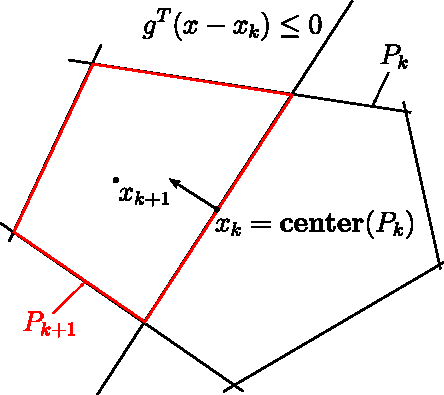
\includegraphics[scale=1.1]{cutting/cuttingregular.pdf}
\par\end{centering}
\caption{Illustration of a shallow cut with an inexact epigraphical oracle. The dotted
line is $f(x)$, the polytope defined by the black solid lines $P_k$. The black
dot is center, and the two red lines are the two cutting planes provided by the 
oracle.} \label{fig:approx-oracle}
\end{figure}

\begin{algorithm} 
  \setstretch{1.2}
  \SetKwInOut{Input}{input}\SetKwInOut{Output}{output}
  \SetKwProg{Fn}{function}{}{end}
  \SetAlgoNoLine
  \DontPrintSemicolon
  $P_0 = C$\;
  
  \While {$\mbox{\normalfont size}(P_k)^{1/(n+1)} \geq \mbox{TOL}$} {
  \nl $x_{k}  = \mathbf{center}(P_k)$\;
  \nl $g_k = \oracle(x_k)$\;
  \nl $P_{k+1} = P_k \cap \{x \mid g_k^T(x -x_k) \leq 0 \}$\;
  \nl $k = k + 1$
  }
  \caption{Cutting Plane Method \label{alg:cutting_plane}}
\end{algorithm}

There are many choices for $\mathbf{center}$, but the main aim is that all
hyperplanes through it partition the set into two approximately
evenly parts. A classical choice is the center of gravity
$$
\mbox{\bf center}(P) := \mbox{center of gravity of $P$} = \frac{\int_P z dz}{\int_P dz}
$$
Just the way the midpoint of a line segment
splits it evenly into two parts, Grunbaum's theorem states that
any splitting of a convex $P$ into two parts will slice it into parts
at most $\exp(-1)$ and $1- \exp(-1)$.


\begin{figure} 
\begin{centering}
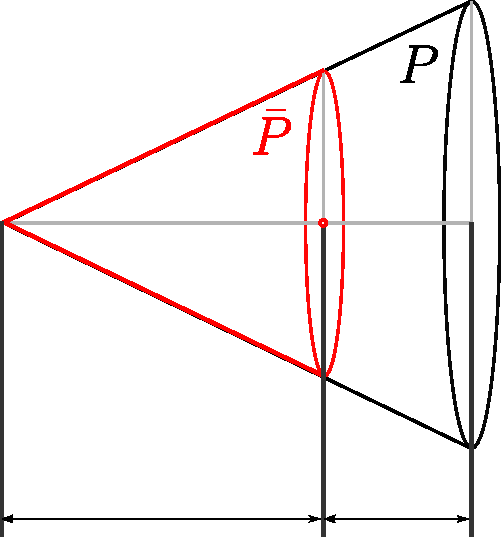
\includegraphics[scale=0.65]{cutting/cog_worstcase.pdf}
$\qquad\qquad$
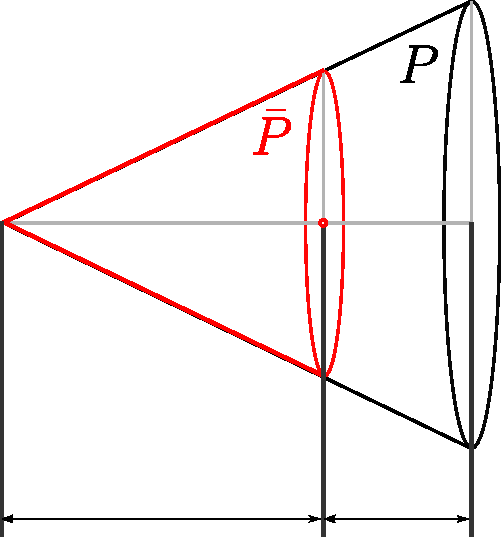
\includegraphics[scale=0.65]{cutting/cog_worstcase.pdf}
\par\end{centering}
\caption{Worse case.} \label{fig:worst-case}
\end{figure}

\begin{thm} {\bf (Grunbaum's Theorem)} \label{thm:CG_cut} 
Let $a$ be the center of gravity of $P$. Then for any $g$,
$$
 0.367 < \frac{1}{\exp(1)} \leq \frac{\vol(P \cap \{ x \mid g^T(x - a)\leq 0\}) }{\vol(P)} \leq 1- \frac{1}{\exp(1)} < 0.633
$$
\end{thm}



This leads to the center of gravity method,
\cite{levin1965algorithm,newman1965location}, with $\mathbf{center}$
equal to the center of gravity, and for which we can guarantee a shrinkage
in volume of 
$$\frac{\vol(P_k)}{\vol(P_{k+1})} \leq 1 - \frac{1}{\exp(1)} $$ 
at every iteration. Another choice for the center is the center of the
maximally inscribed ellipsoid inside a convex set $P$. Then we have a
similar gurantee, with a mildly smaller convergene rate:

\begin{thm} \label{thm:MIE_cut} \cite{tarasov1988method} 
Let $\mathcal{E}$ be the maximum volume ellipse of $P$. Then for any $g$,
$$
\frac{\volmu(P \cap \{ x \mid g^T(x - a)\leq 0\}) }{\volmu(P)} \leq 0.843  
$$
where $a$ is the center of $\mathcal{E}$.
\end{thm}

Note, however, that the MIE is solvable by an SDP, and hence is far
more computationally tractable than the center of gravity. Other 
methods for computing the center exist, including  the volumetric center
\cite{vaidya1989new}, and the analytic center \cite{ye1996complexity}.

Let us now translate the volume decrease into a concrete condition on
the optimality of the problem. For our purposes
it is helpful to define a slightly more general notion of volume, a
$d$-measure. $\volmu$ is a $d$-measure if the volume increases relative to
inclusion, $P_1 \subseteq P_2 \Rightarrow \mu(P_1) \leq \mu(P_2)$, it is
homogenious with respect to scaling, i.e. $\mu(a+AP)=\det(A)\mu(P)$. Two such
measures of $\mu$ used in this paper are the volume of $\mu$ and the volume of
the maximum inscriped ellipse of $P$. The following Lemma is an adaptation of
a remark in \cite{tarasov1988method}, with the proof added for completeness.

\begin{lem}\label{lem:lem-voldecrease} Let $P$ be a convex polytope containing $x^*$. Then there exists a point on the boundary of $P$, $\bar{x}$ such that
$$
f(\bar{x})-f(x^{*})\leq\left(\max_{x\in C}f(x)-\min_{x\in C}f(x)\right)\left(\frac{\mu(P)}{\mu(C)}\right)^{1/d}
$$
\end{lem}
\begin{proof}
Following \cite{tarasov1988method}, let
$\alpha^\star = \max_{a\in\lambda}\left\{ \alpha\mid\alpha\geq0,x^*+\alpha C\subseteq P\right\}.$ 
Let $x\submax = \mbox{argmax}_{x\in C} f(x)$. Let $\bar{x}$ be the point in which the line $[x^*, x\submax ]$ intersects $P$. Then
\begin{align*}
f(\bar{x})-f(x^{*}) & \overset{(a)}{\leq}\left(f(x\submax)-f(x^{*})\right)\frac{\|\bar{x}-x^{*}\|}{\|x\submax-x^{*}\|}\\
 & \overset{(b)}{\leq}\left(f(x\submax)-f(x^{*})\right)\alpha^\star
 \overset{(c)}{\leq}\left(f(x\submax)-f(x^{*})\right)\left(\frac{\volmu(P)}{\volmu(C)}\right)^{1/n}.
\end{align*}
$(a)$ comes from the fact that $$\frac{f(y)-f(x)}{\|y-x\|}\leq\frac{f(z)-f(x)}{\|z-x\|} \qquad x \in [y,z].$$$(b)$ comes from the fact that and $x^* + \alpha C \subseteq P$, and $(c)$ comes from the fact that $\alpha^n \mbox{vol}(C) =  \mbox{vol}(\alpha C) \leq \mbox{vol}(P).$
\end{proof}


Observe that for all cutting plane methods, including the ellipsoid method, $\min\{f(x_1),\dots, f(x_k)\}$ is smaller than all the points in the perimeter. Therefore we can use the above theorem to effectively determine rates of convergence. The convergence rate we get is
$$
\min\{f(x_{1}),\dots,f(x_{k})\}-f(x^{*})\leq \mbox{rate}^{k/n}\cdot\left(\max_{x\in C}f(x)-\min_{x\in C}f(x)\right)
$$

where $\mbox{rate}$ is $1 - 1/\exp(1)$ for the center of gravity method, and
$0.843$ for the Maximum Inscribed Ellipsoid method.

Cutting-plane algorithms enjoy a number of attractive properties that
set them apart from other first-order methods.  Firstly, for a fixed
dimension, the center of gravity and maximum inscribed ellipsoid
variants achieve optimal oracle complexity, up to a constant factor
\cite{nemirovski1994efficient}. Secondly, on any convex function, they
achieve a universal, linear rate of convergence
\cite{nemirovski1994efficient}. This rate of convergence,
surprisingly, is oblivious to the structure of the function itself.

These advantages come at a price. Firstly, each step of the cutting
plane algorithm requires the computation of ${\bf center}$, which may
exceed the cost of the original problem. Furthermore, though the
convergence rates of cutting plane algorithms do not depend on the
conditioning of the problem, it depends strongly on the dimension of
the problem, sometimes degrading exponentially as the dimensions
increase. It is for these reasons that these algorithms are not
practical for problems of any substantial dimension.


\subsubsection{Ellipsoid Methods}

\begin{figure} 
\begin{centering}
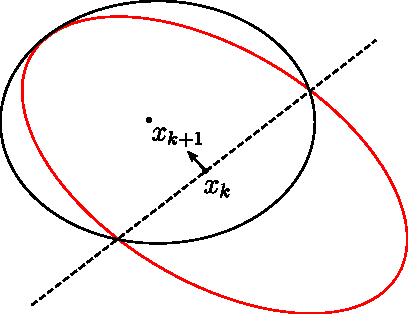
\includegraphics[scale=1.1]{cutting/ellipsoid.pdf}
\par\end{centering}
\caption{Illustration of a shallow cut with an inexact epigraphical oracle. The dotted
line is $f(x)$, the polytope defined by the black solid lines $P_k$. The black
dot is center, and the two red lines are the two cutting planes provided by the 
oracle.} \label{fig:approx-oracle}
\end{figure}

The Ellipsoid method \cite{bland1981ellipsoid} is proposed as a solution
to the large amount of effort needed in computing the center, and 
proposes an interesting compromise between the amount of work required
at each iteration and the overall convergence rate in terms of the
number of calls to the oracle. Instead of 
using a polyhedral representation, which stores all the information
from previous iterations, we use an Ellipse as the
localization polytope. Then, each time new information about where the
optimum is given, the ellipse is updated. Define an ellipsoid as
$$\mathcal{E} = \{ x \mid (x - \bar{x})^T E^{-1} (x - \bar{x}) \leq 1\}$$
The ellipsoid algorithm works due to a the following fact about $n$-dimensional ellipses

\begin{fact} Let $\mathcal{E}$ be an ellipsoid $
\mathcal{E} = \{ x \mid (x - \bar{x})^T E^{-1} (x - \bar{x}) \leq 1\} 
$ and $\mathcal{E}^+$ be the smallest ellipsoid containing $\mathcal{E} \cap \{ x \mid g^T(x - \bar{x}) \leq 0\}$.
Then, $ \mathcal{E^+} = \{ x \mid (x - x^+)^T[E^+]^{-1} (x - x^+) \leq 1 \} $,
$$
x^{+} =x-\frac{1}{n+1}\cdot\frac{1}{\sqrt{g^{T}Pg}}\cdot Pg, \qquad
P^{+} =\frac{n^{2}}{n^{2}-1}\left(P-\frac{2}{(n+1)}\cdot\frac{1}{g^{T}Pg}Pgg^{T}P\right)
$$
Furthermore, 
$$\frac{\vol (\mathcal{E}^+)}{\vol (\mathcal{E})} \leq \exp\left(-\frac{1}{4n}\right)$$
\end{fact}

The fact that we have a guaranteed geometric shrinkage of ellipsoids is constant suggests
a immediate algorithm. We maintain a sequence of ellipsoids, $\mathcal{E}_k$, each which contain
$x^*$. Each call to the gradient oracle yields a cutting plane which splits the ellipsoid into two parts,
and the next ellipsoid is the best ellipsoidal approximation to the half ellipsoid. 
\begin{algorithm} 
  \setstretch{1.2}
  \SetKwInOut{Input}{input}\SetKwInOut{Output}{output}
  \SetKwProg{Fn}{function}{}{end}
  \SetAlgoNoLine
  \DontPrintSemicolon
  $P_0 = C$\;
  
  \While {$\mbox{\normalfont size}(\mathcal{E}_k)^{1/n} \geq \mbox{TOL}$} {
  \nl $x_{k}  = \mathbf{center}(\mathcal{E}_k)$\;
  \nl $g_k = \oracle(x_k)$\;
  \nl $\mathcal{E}_{k+1} = \mbox{minimal ellipse containing }\mathcal{E}_k \cap \{x \mid g_k^T(x -x_k) \leq 0 \}$\;
  \nl $k = k + 1$
  }
  \caption{Ellipsoid Method \label{alg:ellipsoid}}
\end{algorithm}

The algorithm above was written as in a way which is suggestive of cutting
point algorithms. But we can also write the method as an iteration without any
references to Ellipses at all.
\begin{align*}
(u_k,g_{k}) & =\oracle(x_{k})\\
x_{k+1} & =x-\frac{1}{n+1}\cdot\frac{1}{\sqrt{g_{k}^{T}P_{k}g_{k}}}\cdot P_{k}g_{k}\qquad
P_{k+1}  =\frac{n^{2}}{n^{2}-1}\left(P-\frac{2}{(n+1)}\cdot\frac{1}{g_{k}^{T}Pg_{k}}Pg_{k}g_{k}^{T}P\right)
\end{align*}
Though discovered by Shor, Iudin and Nemirovskii \cite{bland1981ellipsoid},
this method got its claim to fame when it was observed that these updates are
numerically stable on fixed precision machines. And hence, the method could
be adapted, via computations on fixed precision machines, to solve the linear
programming problem. This algorithm thus resolved a longstanding issue of the
complexity class of linear programming, putting it squarely in complexity
class $P$.

The convergence rate of the Ellipsoid method can be obtained via Lemma
\ref{lem:lem-voldecrease} with $\mbox{rate} = \exp(-1/4n)$. Note that unlike
the center of gravity or the maximum inscribed ellipsoid method, the rate at
which the volumes decrease depends on the $n$, the dimension of the problem,
degrading exponentially as $n$ goes up. For this reason, it is generally
considered to be inferior to the classical classical cutting point methods,
and generally performs poorly in practice.

\subsection{Epigraphical cutting plane algorithms}

One shortcoming of the algorithm described above is that it does not make
use of the objective value, and discarding this information seems
wasteful. One way to incoperate information about the objective
 involves using deep cuts. To begin, we keep track of our best objective value thus far,
which is also the best upper bound on $\inf f(x)$
$$
u^*_k = \min{ \{ u_0, \dots, u_{k-1}\} } \;\; \mbox{ (best upper bound on optimal objective)} 
$$
Then for $(u, g_k) = \oracle(x_k)$, if our objective value is not smaller
than the original objective, we instead using the deeper cut
$$
g^T(x - \bar{x}) \leq u - u^*_k
$$
This method employs information on the objective value 
$$
l^*_k(x) = \max_{i < k}\{l_i + g_i^T(x-x_i)\} \;\; \mbox{ (best lower bound on $f$)}
$$
Though these methods do incoperate information about the upper bound,the epigraphical cutting plane method, first suggested in
\cite{bahn1994experimental} and also described in
\cite{boyd2007localization,goffin1999two,mehrotra2000volumetric} is an elegant
solution which incoperates both information about the lower bound and the 
uncertainty around the objective value.

This oracle gives us a global lower minorant for $f$, $u + g^T(\cdot - x) \leq t$ and an upper bound on the $f(x^*)$, $u$. Operating on the lifted space $(t,x)$, the epigraphs of these two linear functions form the cutting planes which separate the current iterate $(t_k, x_k)$ from the solution, $(f(x^*), x^*)$. 
\begin{algorithm} 
  \setstretch{1.2}
  \SetKwInOut{Input}{input}\SetKwInOut{Output}{output}
  \SetKwProg{Fn}{function}{}{end}
  \SetAlgoNoLine
  \DontPrintSemicolon
  $P_0 = C$\;
  
  \While {$\mbox{\normalfont size}(P_k)^{1/(n+1)} \geq \mbox{TOL}$} {
  \nl $x_{k}  = \mathbf{center}(P_k)$\;
  \nl $(u_{k},g_{k})  = \oracle(x_{k})$\;
  \nl $P_{k+1}  =P_{k}\cap\{(t,x)\mid t\leq u_{k}\}\cap\{(t,x)\mid l_{k}+g_{k}^{T}(x-x_{k})\leq t\}$\;
  \nl $k = k + 1$
  }
  \caption{Epigraphical Cutting Plane Methods \label{alg:cutting_plane_epi}}
\end{algorithm}

Unlike the cutting plane algorithm, these two half-spaces generally do not
pass through the search point $(t_k, x_k)$. It is guaranteed, however, to do
at least better, and cut off the search point. And the cuts are typically deep - they truncate more than is strictly needed, to achieve a greater volume reduction. This comes at the price, however, of lifting the problem an extra dimension.

For the epigraphical variants of the cutting plane algorithm, we have the following analogous lemma

\begin{lem} \label{lem:non_strongly_convex_convergencegen}
Let  $\mathcal{K}=\mbox{{\rm conv}}\{\sup_{x\in C} f(x) \times  S,(f(x^*),x^*)\}.$
Then for an epigraphical polytope $$P =\{(t,x)\mid t\leq u^*\}\cap \mbox{\normalfont epi}(l), \qquad \mbox{for some convex lower bound $l$ on $f$}
$$
Then \[
u^*-f(x^*)\leq \left(\max_{x\in C}f(x)-\min_{x\in C}f(x) \right) \left( \frac{\volmu(P)}{\volmu(\mathcal{K})} \right)^{1/(n+1)}
\]
\end{lem}
\begin{proof}
Let $\mathcal{K}_k =\mathcal{K}\cap\{(t,x)\mid t \leq u^*_k\}$. Then 
\[
  \volmu(P_k)\overset{(a)}{\geq}\volmu(\mathcal{K}_k)\overset{(b)}{=}
  \left(\frac{u^*_k-f(x^*)}{\max_{x\in C} f(x) -f(x^*)}\right)^{n+1} \!\!\!\!\!\!\!\!\!\cdot \volmu(\mathcal{K}_0)
\]
$(a)$ comes from the fact, $P_k\supseteq \mathbf{epi}(f) \cap \{(t,x) \mid t \leq u_k\} \supseteq \mathcal{K}_k$ and
$\volmu(A)\leq\volmu(B)$ when $A\subseteq B$. $(b)$ comes from the fact
that $\mathcal{K}_k$ is just $\mathcal{K}_0$ scaled about the
base, and $\volmu(\alpha A)=\alpha^{d}\volmu(A)$.
Taking powers of $1/(n+1)$ on both sides, we yield the desired result.
\end{proof}

Just like the cutting plane methods, we can prove the following bound
$$
\min\{f(x_{1}),\dots,f(x_{k})\}-f(x^{*})\leq \mbox{rate}^{k/(n+1)}\cdot\left(\max_{x\in C}f(x)-\min_{x\in C}f(x)\right)
$$

where $\mbox{rate}$ is $1 - 1/\exp(1)$ for the center of gravity method, and
$0.843$ for the Maximum Inscribed Ellipsoid method. Note that though these
bounds are slightly worse than those of the cutting plane methods, they
do not account for the fact that we are using two cutting planes for the 
volume reduction, not one, and that these two planes cutts are typically deep.
Since deep cuts cut off more of the polytope than is strictly needed, the 
volume reduction is significantly greater.

\subsubsection{Bundle Methids}
These methods have strong connections to bundle methods.  Kelly's method
\cite{kelley1960cutting} produces the next iterate by minimizing $l^*_k$
directly. Bundle methods \cite{lemarechal1975extension,wolfe1975method}
regularize this approach work by minimizing $l_k^*$ with a quadratic term. A
generic bundle method looks like this

\begin{algorithm} 
  \setstretch{1.2}
  \SetKwInOut{Input}{input}\SetKwInOut{Output}{output}
  \SetKwProg{Fn}{function}{}{end}
  \SetAlgoNoLine
  \DontPrintSemicolon
  $P_0 = C$\;
  
  \While {$\mbox{\normalfont size}(P_k)^{1/(n+1)} \geq \mbox{TOL}$} {
  \nl $x_{k}  = \mbox{argmin } l_k^*(x) + \tfrac{1}{2}\|x - x_{k-1}\|^2$\;
  \nl $(u_{k},g_{k})  = \oracle(x_{k})$\;
  \nl $l^*_{k+1}  = \max\{l^*_k, l_k + g_k^T(\cdot-x_k)\}$\;
  \nl $k = k + 1$
  }
  \caption{Bundle Method \label{alg:bundle}}
\end{algorithm}

The algorithm above does not do the justice to the vast literature on bundle methods,
but it suffices to give a taste of it. Talk about Bundle Reductions, blah blah blah.

Though the subproblems involved in bundle methods are typically a lot more tractable
than those in the cutting plane methods - the theoretical covnergence for these methods
are typically on the order of subgradient descent. They dramatically outperform
subgradient descent, however, in practice.

\subsection{Proximal Methods}

\subsubsection{Smooth Functions with Composite Structure} While smooth
optimization is useful in itself, we can, with a little effort, add a  small
amount of structurally simple nonsmoothness. We will consider the minimization
of problems with additive composite structure, i.e.
\begin{equation}
  \label{eq:minimize_fpg}
  \underset{x\in {\Real}^n}{\text{minimize}} \quad f(x) + g(x)
\end{equation}
Here we consider functions $f:\Real^n\to\Real$ and
$g:\Real^n\to\Real\cup\{+\infty\}$. Here $f$ is assumed to be smooth, and $g$
is usually simple. In machine learning applications, typically, $f$ is a loss
function that penalizes incorrect predictions of a model. $f$ contains the
data, and is typically hard to compute - but is smooth. $g$ is a regularizer
that encourages desirable structure in the solution. Important examples of
nonsmooth regularizers are the 1-norm and total variation, which encourage
sparsity in either $x$ or its gradient. Let us explore a few examples of functions
with composite structure.

\begin{example}[Feature Selection] 
The feature selection problem considers the case where
only a subset of the features are informative. The rest have no
predictive value, and should be omitted to obtain the most
parsimonious model. 
\end{example}

\begin{example}[Total Variation Denoising]

\begin{equation}
\mbox{minimize}\qquad \underset{f(x)}{\underbrace{\frac{1}{2}\|x-b\|^{2}}}+\underset{g(x)}{\underbrace{\lambda\|Ax\|_{1}}}\end{equation}
\end{example}

\begin{example}[Support Vector Machines]
\[
\mbox{minimize}\qquad
\underset{f(x)}{\underbrace{\mathbf{1}^{T}x-\frac{1}{2}\|A^{T}x\|^{2}}}+
\underset{g(x)}{\underbrace{\delta(x\mid \{ z \mid 0\leq z\leq w_{\lambda} \})}},
\qquad\delta(x|S)=\begin{cases}
0 & x\in S\\
\infty & x\notin S
\end{cases}
\]

\end{example}

\subsubsection{Descent Algorithms for Composite Problems}
When $f$ is smooth,
our oracle gives us gradient information, which can be interpreted as decrease
if we move an tiny amount in $d$
$$
\nabla_x f(x) = \lim_{\epsilon \rightarrow 0}\max_d f(x + \epsilon d)
$$
This information is exploited in descent methods, such as gradient
descent and its accelerated versions. In these algorithms, we make a 
small step in a descent direction - and secure a small, local amount
amount of function decrease at every iteration. 
$$
x_{k+1} = x_k - \alpha \nabla f(x_k)
$$
We can generalize slightly to problems where $g$ isn't $0$. We begin by
discussing an interpreation of a large class of descent methods popular in
first order optimization. Given a  function $f$, differentiable at $x_k$, our
guess of the solution at  iterate $k$, we can construct a quadratic model
around $k$ as such:
\begin{align*} 
f(x) & \approx f(x_{k})+\nabla f(x_{k})^{T}(x-x_{k})+\frac{1}{2}\|x-x_{k}\|_{H}^{2} =f(x_{k})+\frac{\alpha}{2}\|x-x_{k}-\frac{1}{\alpha}\nabla f(x_{k})\|_H^{2}
\end{align*}
$H$ we will assume is a invertible, quadratic model of curvature. For
different choices of $H$, we obtain

In composite optimization, we do an identical thing. Pulling $g$ 
through and completing the square, we get
\begin{align*}
f(x)+g(x) & \approx f(x_{k})+\nabla f(x_{k})^{T}(x-x_{k})+\frac{1}{2}\|x-x_{k}\|_{H}^{2}+g(x)\\
 & =f(x_{k})+\frac{\alpha}{2}\|x-x_{k}-\frac{1}{\alpha}\nabla f(x_{k})\|_H^{2}+g(x)
\end{align*}
By minimizing the approximation, we get the next iterate. Therefore
$$
x^{+}=\underset{\bar{x}}{\mbox{argmin}}\left\{ 
\frac{1}{2}\|\bar{x}-x-H^{-1}\nabla f(x)\|_{H}^{2}
+g(\bar{x})\right\} 
$$

This is one
motivation for the definition of the proximal operator. The objective
value which the quadratic optimization takes $$
\mathbf{prox}^H_{g}(z):  =\underset{x\in\Real^{n}}{\text{argmin}}\left\{
\frac{1}{2}\|z-x\|_H^{2}+g(x)\right\}, \qquad  \mathbf{env}^H_{g}(z):
=\underset{x\in\Real^{n}}{\text{min}}\left\{
\frac{1}{2}\|z-x\|_H^{2}+g(x)\right\}  $$ And the proximal gradient
iteration is 
\begin{equation}\label{eq:prox-gradient}
x_{k+1}=\mathbf{prox}^\alpha_g(x_k-\alpha^{-1}\nabla f(x_k))
\end{equation}
The connection to gradient descent is clear. If $g=0$, we recover
the descent iteration. Like gradient descent, under reasonable
hypotheses they are guaranteed to achieve, within $k$ iterations, a
function value that is within $\mathcal{O}(1/k)$ of the optimal value
using a constant step size, and within $\mathcal{O}(1/k^2)$ using an
accelerated variant. \cite{Tseng:2010} outlines a unified view of the
many proximal- gradient variations, including accelerated versions
such as FISTA~\cite{beck2009fast}.

For $g$'s which are structurally simple, this it leads to an
inexpensive proximal iteration. This is not limited to, but
particularly true in the case where $g$ is separable.

When gradients of $f$ are expensive to compute, incorporate into our iterations some approximation of curvature. Suppose that $H$ is a positive-definite matrix. The iteration
\begin{equation}
  \label{eq:prox-map}
  x^{+}={\bf{prox}}^H_g(x-H^{-1}\nabla f(x))
\end{equation}
is a generalization of proximal-gradient, where $x$ is most
recent estimate of the solution, and
\begin{equation}
  \label{eq:2}
  {\bf{prox}}^H_g(z):=\underset{x\in {\Real}^n}{\text{argmin}} 
  \left\{
  \tfrac{1}{2}\|z-x\|_H^{2}+g(x) \right\}
\end{equation}
is the (scaled) proximal operator of $g$. The scaled diagonal
$H=\alpha I$ is the vanilla proximal operator described
in the previous sections. For more general matrices $H$, however,
may lead to proximal operators that dominate the computation. The
choice of $H$ remains very much an art - we are trading off complexity
in the inner subproblems for less calls to the gradient of $f$. There is an entire
continuum of algorithms that vary based on the choice of $H$, as
illustrated by Table~\ref{tab:methods}.
\begin{table}
  \caption{Preconditioned proximal-gradient methods.}
  \centering
  \begin{tabular}{l|l|l}
    %\toprule
    Method & Reference & $H$\\
    %\\\midrule
    iterative soft thresholding & \cite{beck2009fast} & $\alpha I$
    \\symmetric rank 1 & \cite{NIPS2012_4523} & $\alpha I+ss^{T}$
    \\identity-minus-rank-1 & \cite{1401.4220}  &$\alpha I-ss^T$
    \\proximal L-BFGS &\cite{schmidt2009optimizing,NIPS2014_5384,Scheinberg2016} &$\Lambda+SDS^{T}$
    % \\preconditioned proximal gradient & &$\approx\nabla^2 f(x)$ is easily invertable
    \\proximal Newton &\cite{lee2014proximal,JMLR:v16:trandihn15a,Byrd2016} & $\nabla^{2}f$
    %\\\bottomrule
  \end{tabular}
  \label{tab:methods}
\end{table}

Thee table lists a set of algorithms roughly in order of the accuracy
with which $H$ approximates the Hessian---when it exists---of the
smooth function $f$. At one extreme is iterative soft thresholding
(IST), which approximates the Hessian using a constant diagonal. At
the other extreme is proximal Newton, which uses the true Hessian. The
quality of the approximation induces a tradeoff between the number of
expected proximal iterations and the computational cost of evaluating
the proximal operator at each iteration. Thus $H$ can be considered a
preconditioner for the proximal iteration. The proposals offered by
\cite{JMLR:v16:trandihn15a} and \cite{Byrd2016} are flexible in the
choice of $H$, and so those references might also be considered to
apply to other methods listed in Table~\ref{tab:methods}.


\section{Algorithms with Inexact Oracles}


\subsection{Inexact cutting plane algorithms}

The following oracle captures such cases by only requiring an approximate
subgradient, as defined by an
$\epsilon$-subgradient~\cite[p.~219]{Roc70}.

The $\epsilon$-subgradient, too, gives us a hyperplane that separates
$x$ from $x^*$. However, this hyperplane is not guaranteed to pass
through $x$ because
\[
f(\bar{x})\geq f(x) \geq f(x^*) \quad\forall \bar{x} \quad \text{such that} \quad g^T(\bar{x}-x)\geq\epsilon, \quad g \in \partial_\epsilon f(x).
\]
If we assume for the moment that $g\ne0$, then $g^T(\bar{x}-x)$
and so we observe that the hyperplane defined by the
$\epsilon$-subgradient is displaced from $x$ in the normalized
direction $g/\|g\|$ by the amount $\epsilon/\|g\|$ from $x$. The
smaller the distance $\epsilon/\|g\|$, the more the halfspace slices
off $P$. Therefore this motivates the definition of a scaled inexact
oracle wherein we control directly the distance the hyperplane lies
from $\epsilon$.

This definition bears resemblance the definition of the shallow-cut
oracle described in the classical literature on shallow-cut ellipsoid
methods \cite{bland1981ellipsoid,grotschel2012geometric}. The main
difference is the norm in which $g$ is measured. Algorithms which use
inexact cutting planes follow this pattern. We start with
$P_0 = \mathcal{C}$. Then
\begin{algorithm} 
  \setstretch{1.2}
  \SetKwInOut{Input}{input}\SetKwInOut{Output}{output}
  \SetKwProg{Fn}{function}{}{end}
  \SetAlgoNoLine
  \DontPrintSemicolon
  $P_0 = C$\;
  
  \While {$\mbox{\normalfont size}(P_k)^{1/(n+1)} \geq \mbox{TOL}$} {
  \nl $x_{k}  = \mathbf{center}(P_k)$\;
  \nl $g_{k}  = \shalloworacle(x_{k}, \epsilon)$\;
  \nl $P_{k+1} = P_k \cap \{x \mid {g_k}^T({x -x_k}) \leq \epsilon\|g\|\}$\;
  \nl $k = k + 1$
  }
  \caption{Cutting Plane Methods \label{alg:shallow_cutting_plane}}
\end{algorithm}
First, a center is chosen. And then, a shallow cut oracle is called
with a specific $\epsilon_k$, one typically determined by $P_k$, to
ensure a consistent rate of decrease. When $\mathbf{center}$ is the
center of gravity, for example, Bertsimas and Vempala
\cite[Theorem~3]{bertsimas2004solving} give a bound on the guaranteed
proportion of decrease in volume if the cutting plane misses the
center of gravity by a distance $\epsilon$.


\subsubsection{Inexact Bundle Methods}

\subsubsection{}

\section{Algorithms with Stochastic Oracles}

\begin{equation}\label{eq:grad-descent}
x_{k+1} = x_k - \alpha g_k
\end{equation}

The use of stochastic oracles have its earliest beginnings in stochastic
approximation. For smooth functions, the approximate gradient is used
as a drop in replacement of the true gradient

In general, if $\lim\inf_{k} \|e_{k}\| \neq 0$, then we necessarily
require $\alpha_k\to0$ in~\eqref{eq:grad-descent} in order to ensure optimality
of limit points. \cite[Theorem~3.4]{ComWaj2005}
show that the iteration~\eqref{eq:grad-descent} converges to a solution when
$0<\inf\alpha_k<\sup\alpha_k<2/L$ and
$\sum_{k\in\mathbf{N}}\|{e_k}\|<\infty$, and also consider other kinds
of perturbations that enter into the iteration; no convergence rates
are given.  \cite{SchmidtRouxBach:2011} link
the convergence rate of the iterations (including accelerated
variants) to $\mathbf{E} \|e_{k}\|^{2}$, which measures the variance in the
error, and to error in the computation of the projection. In the case in
which $e_k=0$ has zero mean and finite variance, it is known that the
projected-gradient method converges as $\mathcal{O}(1/\sqrt k)$; see, e.g.,
\cite{Langford:2009:SOL:1577069.1577097}. Contrast these rates
to those that can be obtained when $e_k\equiv0$, and in that case the
method has a rate of $\mathcal{O}(1/k)$, and its accelerated variant has a
rate of $\mathcal{O}(1/k^2)$, which is an optimal rate; see, e.g.,
\cite{Nes07} and \cite{BeT08}.

For the case where $g\equiv0$ (and hence the projection operator
in~\eqref{eq:grad-descent} is simply the identity map), has been extensively
studied. It is well known that if $f$ is strongly convex,
deterministic steepest descent without error (i.e., $e_k\equiv0$) and
with a constant stepsize $\alpha_k = 1/L$ converges linearly with a
rate constant $\rho<1$ that depends on the condition number of $f$;
see \cite[section~8.6]{luenberger2008linear}. \cite{BT:2000} describe conditions for convergence of the
iteration~\eqref{eq:grad-descent} when the steplengths $\alpha_k$ satisfy the
conditions $\sum_{k\in\mathbf{N}} \alpha_k = \infty$ and
$\sum_{k\in\mathbf{N}} \alpha_k^2 < \infty$. \cite{NedBer:2000} show that randomized incremental-gradient
methods for~\eqref{eq:29}, with constant steplength
$\alpha_k\equiv\alpha$, converge as 
\[ \mathbf{E}\pi_k \le \mathcal{O}(1)(\rho^k +
\alpha) \] 
where $\mathcal{O}(1)$ is a positive constant. This expression is
telling  because the first term on the right-hand side decreases at a
linear rate, and depends on the condition number through $\rho$; this
term is also present for any deterministic first-order method with
constant stepsize. For a constant stepsize, \cite{friedlander2012hybrid} give non-asymptotic rates that directly
depend on the rate at which the error goes to zero, and for the case
where $f$ is given by~\eqref{eq:29}, they further show the dependence
of the convergence rate on the sample size.


For a non-vanishing stepsize, i.e., $\liminf_{k}\alpha_k>0$,
\cite{luo1993error} show that for a decreasing error sequence that satisfies
$\|e_{k}\| = \mathcal{O} ( \|x_{k+1}-x_{k}\|)$, the function values converge to the
optimal value at an asymptotic linear rate.

The convergence in probability of the stochastic-approximation method
was first discussed by the classic 
\cite{robbins1951stochastic} paper. \cite{BT:2000} give mild conditions on $e_{k}$ and $f$
under which $f(x_{k}) \to \inf f(x)$ in probability. More recently,
\cite{nemirovski2009robust}
show that for decreasing steplengths $\alpha_k = \mathcal{O}(1/k)$, these
methods achieve a sublinear rate according to $\mathbf{E}\pi_k =
\mathcal{O}(1/k)$; the iteration average has similar convergence
properties, and it converges sublinearly with overwhelming
probability. A similar effort by \cite{nesterov2008confidence}
give exponential tail bounds for sequences with any steplength
sequence.


\section{Thesis Outline}

   \chapter{The Inexact Epigraphical Cutting Plane Algorithm}
   \label{ch:InexactEpiCuttingPlane}
   %!TEX root = ../Dissertation.tex

\section{The Inexact Epigraphical Cutting Plane Algorithm}

% \begin{figure}

% \noindent\rule[0.1ex]{1\columnwidth}{0.5pt}
% {Inexact Epigraphical Cutting Plane}
 
% \vspace{-2mm}
% \noindent\rule[0.1ex]{1\columnwidth}{0.5pt}

% %\begin{algorithm}
% % \State $P_0 = C \times {[\mbox{upper bound on $f$}, \mbox{lower bound on $f$}]}$
% % \While {$\max\{ \mbox{height}(P_k), K \cdot \mbox{size}(P_k)^{1/(n+1)} \} \geq \mbox{TOL}$}
% %   \State $(t_k,x_k) \gets \mbox{\bf center}(P_k)$
% %   \State $\epsilon_k \gets \gamma (\min \{ u_0, \dots, u_{k-1}\}-t_k )$
% %   \State $(u_k,l_k,g_k)\gets F(x_k, \epsilon_k )$
% %   \State $P_{k+1}\gets P_k\cap 
% %       \underbrace{\{(t,x)\mid t\leq u_k \}}_{\mbox{\tiny upper bound}} \cap 
% %       \underbrace{\{(t,x)\mid l_k+g_k^{T}(x-x_k)\leq t\}}_{\mbox{\tiny lower bound}}$
% %   \vspace{-4mm}
% %   \State $k \gets k+1$  
% % \EndWhile
% %\end{algorithm}
% \noindent\rule[0.1ex]{1\columnwidth}{0.5pt}
% \caption{MVE Epigraphical Cutting Plane Algorithm. $K$ is constant which depends on the $\mbox{\bf center}$, and $\mbox{size}$ is a function which takes convex 
% sets into real values, depending on $\mbox{\bf center}$. } \label{alg:cutting_plane_epi_err}
% \end{figure}

Our proposed algorithm is a modification of the cutting plane algorithms
described in Section [] to accomidate
\begin{algorithm} 
  \SetKwInOut{Input}{input}\SetKwInOut{Output}{output}
  \SetKwProg{Fn}{function}{}{end}
  \SetAlgoNoLine
  \DontPrintSemicolon
  $P_0 = C \times {[\mbox{upper bound on $f$}, \mbox{lower bound on $f$}]}$\;
  
  \While {$\max\{ \mbox{height}(P_k), K \cdot \mbox{size}(P_k)^{1/(n+1)} \} \geq \mbox{TOL}$} {
  \nl $(t_k,x_k) \gets \mbox{\bf center}(P_k)$\;
  \nl $\epsilon_k \gets \gamma (\min \{ u_0, \dots, u_{k-1}\}-t_k )$\;
  \nl $(u_k,l_k,g_k)\gets F(x_k, \epsilon_k )$\;
  \nl $P_{k+1}\gets P_k\cap 
      \underbrace{\{(t,x)\mid t\leq u_k \}}_{\mbox{\tiny upper bound}} \cap 
      \underbrace{\{(t,x)\mid l_k+g_k^{T}(x-x_k)\leq t\}}_{\mbox{\tiny lower bound}}$\;
  \vspace{-5mm}
  \nl $k \gets k+1$  
  }
  \caption{Epigraphical Cutting Plane With Error \label{alg:cutting_plane_epi_err}}
\end{algorithm}
\noindent We will two consider methods of determining $\mbox{\bf center}$, the
center of gravity and the center of the maximum inscribed ellipsoid. In this
section, we will refer to the height of a convex set to be:
$$
\mbox{\rm height}(P)=\max\{t\mid(t,x)\in P\}-\min\{t\mid(t,x)\in P\}.
$$
We will refer to $u^*_k$ as the best upper bound and $l^*_k$ to be the strongest lower bounds.
\[
u^*_k = \min{ \{ u_0, \dots, u_{k-1}\} } \qquad l^*_k(x) = \max_{i < k}\{l_i + g_i^T(x-x_i)\}.
\]
There is an important property of the localization polytopes $P_k$ our method will exploit. Every polytope $P_k$ can be decomposed into the intersection of two sets,
one formed by the intersection of all the lower bounds, other a halfspace
formed by the intersection of the upper bounds, i.e.
$$
P_k = \mbox{epi}(l^*_k) \cap \{(t,x) \mid t \leq u^*_k\}
$$
The level sets of an epigraph are nested, and $\{x \mid (t,x) \in P_k\} $ is the level set of $l^*$ lower bound at $t$,
\[
t_1 \leq t_2 \Rightarrow \{x \mid (t_1,x) \in P_k\} \subseteq \{x \mid (t_2,x) \in P_k\}
\]
and thus every vertical half line emanating from inside the polytope will
only exit the polytope at the upper bound. We will refer to this as $P_k$ tapering downwards.


% $$
% \frac{u_0-f(x^*)}{\volmu(\mbox{conv}\{u_0\times\mbox{lvl}(f,u_0),(f(x^*),x^*)\})^{1/(n+1)}}.
% $$

% \noindent\rule[0.5ex]{1\columnwidth}{0.5pt}
% \begin{enumerate}
%   \item $P_0\supseteq\mbox{epi}(f)$
%   \item While $\max\{ \mbox{height}(P_k), K\volmu(P_k)^{1/(n+1)} \} \geq\epsilon$
%   \begin{enumerate}
% %   \item $\mathcal{E}_k=\mbox{maximum inscribed ellipse of }P_k$
%     \item $(t_k,x_k) = \mbox{\bf center}(P_k)$
%     \item $(u_k,l_k,g_k)=F(x_k,\tfrac{1}{50}(t_k - u_{k-1}))$
%     \item $P_{k+1}=P_k\cap 
%       \underbrace{\{(t,x)\mid t\leq u_k \}}_{\mbox{\tiny lower bound}} \cap 
%       \underbrace{\{(t,x)\mid l_k+g_k^{T}(x-x_k)\leq0\}}_{\tiny \mbox{upper bound}}$
% \end{enumerate}
% \end{enumerate}
% \vspace{1mm}
% \noindent\rule[0.5ex]{1\columnwidth}{0.5pt}

\subsection{The Center of Gravity Oracle} 

We begin our exposition with a conceptual algorithm. For this section
only, define
$$
\mbox{\bf center}(P) := \mbox{center of gravity of $P$} = \frac{\int_P z dz}{\int_P dz} \quad \mbox{and} \quad \mbox{size}(P) = \vol(P).
$$
This definition is valid when $P$ is bounded and has a nonempty interior,
which is true for all localization polyopes. The following theorem establishes
an important geometric fact about the CG.

\begin{thm} {\bf (Grunbaum's Theorem)} \label{thm:CG_cut} 
Let $a$ be the center of gravity of $P$. Then for any $g$,
$$
 \frac{1}{\exp(1)} \leq \frac{\vol(P \cap \{ x \mid g^T(x - a)\leq 0\}) }{\vol(P)} \leq 1- \frac{1}{\exp(1)} 
$$
\end{thm}

The center of gravity can therefore be interpreted as a $n$ dimensional analog
of a midpoint, as it divides a convex set into two approximately equal parts.

\begin{lem}\label{Rate-Decrease_cg}
The volumes decrease at the rate
\[
\frac{\vol(P_{k+1})}{\vol(P_k)}\leq  1-\frac{1-\gamma}{\exp(1)}
\]
\end{lem}
\begin{proof}

\noindent\textbf{Case 1: (Deep Cut) $l_k \geq t_k$ or $l_k \leq t_k$ and $u_k \leq t_k$ } 
The intersection of the cutting planes do not contain $(t_k,x_k)$, therefore by Theorem \ref{thm:MIE_cut},
\[
\frac{\vol(P_{k+1})}{\vol(P_k)}\leq 1 - \frac{1}{\exp(1)}
\]
\textbf{Case 2: (Shallow Cut) $l_k < t_k$ and $u_k > t_k$}. 
See Figure \ref{fig:shallow-cut} for an illustration of this case. 
By the definition of $\epsilon$,
\[
u_k-t_k \leq u_k-l_k\leq \gamma(u^*_k - t_k) \quad \Rightarrow \quad t_k + \gamma(u^*_k - t_k) \geq u_k 
\]
Define $\bar{P}_k$ to be the region above the upper cutting plane, compressed 
by a small amount from the top
\begin{align*}
\bar{P}_k & = \Sigma \big(P_{k}\cap\{(t,x)\mid t\geq t_{k}\} - (u^*_k, 0, \dots, 0) \big) + (u^*_k, 0, \dots, 0) \\
\Sigma & =\mbox{diag}(1-\gamma,1,\dots,1)
\end{align*}
The bottommost point of $\bar{P}_k$ is $(t_k+\gamma(u^*_k-t_k), x_k)$ which lies above $u_k$. Furthermore because the set tapers downwards, so $P_{k}\cap\{(t,x)\mid t\geq u_{k}\} \supseteq \bar{P}_k $. Therefore, taking volumes on both sides
\begin{equation} \label{eq:vol-ineqaality-compression}
\vol(P_k\cap\{(t,x)\mid t\geq u_{k}\})\geq (1-\gamma) \cdot \vol(P_k\cap\{(t,x)\mid t\geq t_{k}\})
\end{equation} 
Now
\begin{align*}
\vol(P_{k+1}) 
 & \overset{(a)}{\leq} \vol(P_k)-\vol(P_k\cap\{(t,x)\mid t\geq u_k\})\\
 & \overset{(b)}{\leq}\vol(P_k)-(1-\gamma)\cdot\vol(P_k\cap\{(t,x)\mid t\geq t_k\})\\
 & \overset{(c)}{\leq}\vol(P_k)-(1-\gamma) e^{-1}\cdot\vol(P_k) 
 = (1 - (1-\gamma)e^{-1} )\cdot \vol(P_k)
\end{align*}
$(a)$ comes from the fact that $P_{k+1}$ is $P_k$ intersected with two cutting planes. The right hand side of $(a)$ is the volume of $P_k$ intersected with just the upper bound. $(b)$ comes from \eqref{eq:vol-ineqaality-compression}. $(c)$ comes from Theorem \ref{thm:CG_cut}. Combing the two results, we obtain the theorem. 
\end{proof}

\begin{figure}
\begin{centering}
\includegraphics[width=0.65\textwidth]{cutting/fig0.pdf}
\par\end{centering}
\caption{Illustration of a shallow cut with an inexact epigraphical oracle. The dotted
line is $f(x)$, the polytope defined by the black solid lines $P_k$. The black
dot is center, and the two red lines are the two cutting planes provided by the 
oracle. \label{fig:shallow-cut}} 
\end{figure}

% \begin{lem} \label{lem:cg_non_strongly_convex_convergencegenc}
% Let $\mathcal{K}_0$ be the cone formed by the level set of $f$ at $u_0$ and the 
% optimal solution, 
% $$\mathcal{K}_{0}=\mbox{{\rm conv}}\{\sup_{x\in S}f(x)\times S,(f(x^{*}),x^{*})\}.$$
% Then for all $k$
% \[
% u^*_{k}-f(x^*)\leq K \cdot \vol(P_{k})^{1/(n+1)}, \qquad K := \frac{u_0-f(x^*)}{\vol(\mathcal{K}_0)^{1/(n+1)}}
% \]
% \end{lem}

% \begin{proof}
% Let $\mathcal{K}_k =\mathcal{K}_0\cap\{(t,x)\mid t \leq u^*_k\}$. Then 
% \[
%   \vol(P_k)\overset{(a)}{\geq}\vol(\mathcal{K}_k)\overset{(b)}{=}
%   \left(\frac{u^*_k-f(x^*)}{u_0-f(x^*)}\right)^{n+1} \!\!\!\!\!\!\cdot \vol(\mathcal{K}_0)
% \]
% $(a)$ comes from the fact that $P_k\supseteq\mathcal{K}_k$. $(b)$ comes from the fact
% that $\mathcal{K}_k$ is just $\mathcal{K}_0$ scaled about the
% base. Taking powers of $1/(n+1)$ on both sides, we get the desired result.
% \end{proof}

Combining the above result with Lemma \ref{lem:non_strongly_convex_convergencegen}, we get a final theorem on the convergence rate of our algorithm.
\begin{thm}\label{thm:MIE-convergence}
For all $k$
\[
u_{k}^{*}-f(x^{*})\leq K\left(1-\frac{1-\gamma}{\exp(1)}\right)^{k/(n+1)}\quad K=(u_{0}-f(x^{*}))\left(\frac{\vol(P_{0})}{\vol(\mathcal{K})}\right)^{1/(n+1)}
\]
and when 
Algorithm \ref{alg:cutting_plane_epi_err} with $\mbox{\bf center}$ being the
center of gravity terminates in no more than
\[
k = \left\lceil \frac{(n+1)\log(K/\mbox{TOL})}{-\log(1-(1-\gamma)/\exp(1))} \right\rceil 
\in \mathcal{O}\left(n\log\frac{1}{\mbox{TOL}}\right).
\]

\end{thm} 

We now focus our attention on the amount of work involved in each
oracle call. Recall that the cost of invoking the oracle is inversely
proportional to $\epsilon_k$. Hence we will show a lower bound on $\epsilon_k$
in the next few lemmas.


\begin{figure}
\begin{centering}
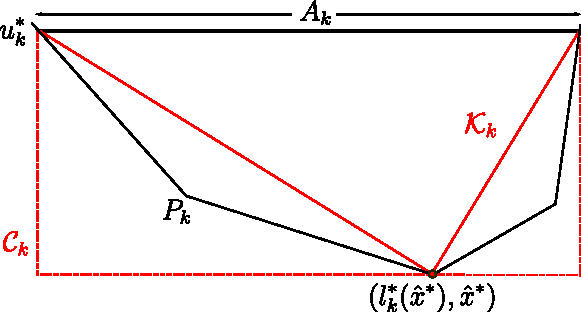
\includegraphics[width=0.65\textwidth]{cutting/fig6.pdf}
\par\end{centering}
\caption{Illustration of outer cylindrical approximation $\mathcal{C}_k$ and inner conic approximation $\mathcal{K}_k$ of $\mathcal{P}_k$} \label{fig:outer-inner-approx}
\end{figure} 

\begin{lem}\label{lem:cg-epsilon-lower-bound}
For all $k$,
\[
\epsilon_k\geq \frac{\gamma \cdot \mbox{\rm height}(P_k)}{(1-\exp(1))(n+1)}
\]
\end{lem}
\begin{proof}
We first construct a conic inner approximation $\mathcal{K}_k$, and a cylindrical outer approximation $\mathcal{C}_k$ of $P_k$. See Figure \ref{fig:outer-inner-approx} for an illustration of these approximations. Let $\hat{x}^*\in \mbox{argmin } l^*_k(x)$, then
\[
\mathcal{K}_{k}:=\mbox{conv}\{u_{k}^{*}\times A_{k},(l_{k}^{*}(\hat{x}^*),\hat{x}^*)\}\subseteq P_{k}\subseteq [l_{k}^{*}(\hat{x}^*),u_{k}^{*}] \times A_{k}=:\mathcal{C}_{k}
\]
Taking volumes of these sets, we get
\begin{align*}
\vol(P_{k}) & \geq\vol(\mathcal{K}_{k}) = \mbox{height}(P_{k})\cdot\vol(A_{k})/(n+1)\\
\vol(P_{k}\cap\{(t,x)\mid t\geq h\}) & \leq\vol(\mathcal{C}_{k}\cap\{(t,x)\mid t\geq h\})=(u_{k}^{*}-h)\cdot\vol(A_{k})
\end{align*}
Here $\vol(A_k)$ refers to the volume of the $n$ dimensional polytope, not the volume of $A_k$ as a set embedded in $n+1$ dimensional space (which is 0). The final inequalities come from the volume of a cone, and a cylinder, respectively. Now,
\begin{align*}
\frac{\epsilon_k(n+1)}{\gamma \cdot \mbox{height}(P_{k})}
& \overset{(a)}{=}\frac{(u_{k}^{*}-t_k)\cdot\vol(A_{k})}{\mbox{height}(P_{k})\cdot\vol(A_{k})/(n+1)}\\
& \overset{(b)}{\geq}\frac{\vol(P_{k}\cap\{(t,x)\mid t\geq t_k\}))}{\vol(P_{k})}
\overset{(c)}{\geq}1-\exp(-1)
\end{align*}
$(a)$ comes from the definition of $\epsilon_k$, $(b)$ from our inner and outer approximating bounds, in particular the outer bound with $h=t_k$. And finally $(c)$ from Theorem \ref{thm:CG_cut}. We obtain the final result from a simple rearrangement.
\end{proof}

\begin{thm} \label{thm:cg-total-work}
Define the total amount of work for each oracle call $F(x,\epsilon) = \epsilon^{-1}$. Assume the algorithm is run till termination. Then the total amount of work involved is
\[
\sum{\frac{1}{\epsilon_{k}}}\leq7\cdot\frac{n+1}{\gamma \mbox{TOL}}\left\lceil (n+1)\log\left(\frac{K}{\mbox{TOL}}\right)\right\rceil \in\mathcal{O}\left(\frac{1}{\mbox{TOL}}\log\frac{1}{\mbox{TOL}}\right)
\]
\end{thm}
\begin{proof}
The algorithm terminates when either
$$
\mbox{height}(P_k)\leq \mbox{TOL} \qquad \mbox{ or }\qquad\vol(P_k)\leq(\epsilon/K)^{n+1} .
$$
Lemma \ref{lem:cg-epsilon-lower-bound} implies the work involved at each
iteration will be no more than $1/(100(n+1)\epsilon)$. Theorem \ref{thm:CG-convergence} gives a bound on the total number of iterations. This gives
\[
\sum {\frac{1}{\epsilon_k}} 
\leq \frac{(1-\exp(-1))(n+1)}{\gamma\mbox{TOL}}
\left\lceil \frac{(n+1)\log(K/\mbox{TOL})}{-\log(1-(1-\gamma)/\exp(1))} \right\rceil
\]
Optimizing for $\gamma$, we get $\gamma \approx 0.473$. Computing the numerical
values and rounding, we obtain the final lower bound.
\end{proof}

\begin{example}[Errors in Epigraphical and shallow-cut oracles]

  This example demonstrates how the amount of work in the epigraphical
  cutting plane scales with the amount of uncertainty in the
  localization polytope. Consider running one iteration of either the
  shallow-cut cutting plane method
  (Definition~\ref{def:shallow-cut-oracle}) or the epigraphical
  variant (Definition~\ref{def:epi-inexact-oracle}) on the one
  dimensional problem
\[
\text{minimum} \quad |x| \quad \text{s.t.} \quad x \geq 0.
\]
We use this problem to compare the amount of work required in a single
call to the oracle for both algorithms. Let $P_x$ be the localization
polytope for the cutting-plane method, and let $\bar{P}_x$ be the
localization polytope for the epigraphical cutting plane. For the
purposes of fair comparison, we will we will assume the uncertainty in
$x$ is fixed, i.e.,
\[
  \bar{P}_x = \{x \mid (t,x) \in P_x\} = [0, x].
\] 

\paragraph{\bf Inexact Cutting Plane} We continue with our running
assumption that evaluating $g \in \partial_\epsilon\|\cdot\|(x)$
requires $1/\epsilon$ amount of work. Note that $g$ is required to satisfy~\eqref{eq:SpO-Oracle}, and thus the oracle requires a cost of $1/(\epsilon \|g\|)$.  We can lower bound the amount of work by upper bounding $\|g\|$, which is $1$ since
\[
  g \in \partial_{\delta}|\cdot|(x)
  =
  \begin{cases}
    [-1,-1-\delta/x] & x\leq-\delta/2
\\   [-1,1]               & -\delta/2< x<\delta/2
\\  [1-\delta/x,1] & x\geq\delta/2.
\end{cases}
\]
Therefore the amount of work required is at least $1/\epsilon$. 
 
\paragraph{\bf Inexact Epigraphical Cutting Plane} To find the tightest
bound on $\epsilon$, we must find the smallest localization polytope
with the property that its projection onto the second coordinate is 
$[0,x]$. This occurs in the triangle
\[
  P_x = \mathbf{epi}(|\cdot|) \cap \{(x,t) \mid t \leq x\}.
\]
Using the well known fact that the centroid of a right angled triangle
lies $1/3$ of the way from the top, the $\epsilon$ which we call our
oracle is $\epsilon = \gamma x/3$, which increases linearly with $x$.
 
While the amount of work when far from $x$ is fixed
in the shallow cut case, it dropes linearly with the size in the epigraphical
case. For a more detailed illustration of the bounds on the amount of work
in the shallow cut oracle, refer to Figure $\ref{fig:bound-errors}$

\begin{figure}
\begin{centering}
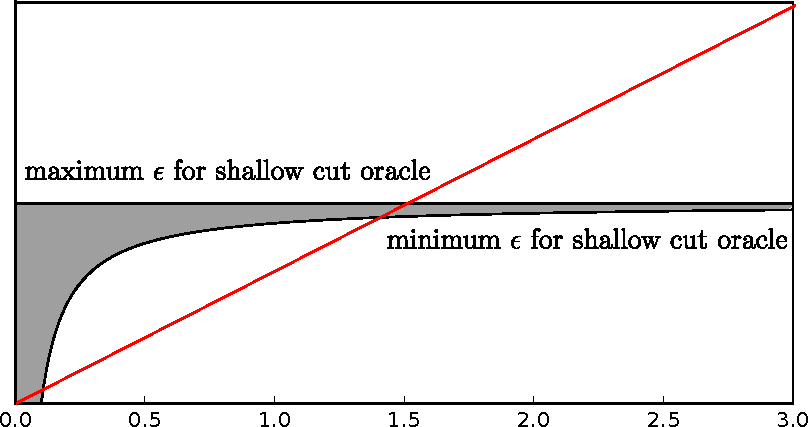
\includegraphics[width=0.65\textwidth]{cutting/epsilon_absx.pdf}
\par\end{centering}
\caption{Bounds on amount of work for shallow cut an epigraphical
cutting plane methods. The shaded gray region represents the
upper and lower bounds for the $\epsilon$ needed in the $\epsilon$-subgradient,
while the red line represents the amount of work needed in the inexact shallow
cut oracle. In epigraphical form, $\epsilon$ increases linearly with the size of the polytope.}\label{fig:bound-errors}
\end{figure} 

\end{example}

\subsection{The Maximum Inscribed Ellipsoid Oracle} 

\cite{tarasov1988method} proposed an alternate oracle as to remedy the problem
of the intractability of the center of gravity. \cite{tarasov1988method} noted
that the center of the  the maximum inscribed ellipse of a polytope shares
many of the properties of the center of gravity, but has the advantage of
being computable in polynomial time. Define an ellipse to be
$$
\mathcal{E} = \{ Ax + a\mid \|x\|\leq 1\}.
$$
Let $P$ be a convex, compact set.  Define the Maximum Inscribed Ellipsoid
(MIE) of $P$ to be ellipse of largest volume contained within $P$. For this
section only, let
$$
\mbox{\bf center}(P) := \mbox{center of MIE of $P$}.
$$
We will
also define $\volmu(P)$ to be to be the volume of this ellipse. Define, for this section only,
$$
\mbox{size}(P) = \volmu(P) = \mbox{max} \{ \vol(\mathcal{E}) \mid \mathcal{E} \mbox{ is an ellipse such that } \mathcal{E}\subseteq P \}
$$
The use of $\mbox{max}$ in place of $\sup$ is justified as the set is compact.
If 
$$P = \{ x \mid g_i^Tx \leq b_i \}$$
The MIE can be computed by solving
$$
\mbox{maximize } \log\det A \qquad \mbox{s.t.}\quad  \|Ag_i\|_2+g_i^Ta \leq b_i
$$
Like the center of gravity, a hyperplane going through the center of the MIE
divides a convex set into two approximately even parts:
\begin{thm} \label{thm:MIE_cut} \cite{tarasov1988method} 
Let $\mathcal{E}$ be the maximum volume ellipse of $P$. Then for any $g$,
$$
\frac{\volmu(P \cap \{ x \mid g^T(x - a)\leq 0\}) }{\volmu(P)} \leq 0.843  
$$
where $a$ is the center of $\mathcal{E}$.
\end{thm}

\noindent
Here we will require a slightly stronger result, Theorem $\gamma$ of
\cite{tarasov1988method}

\begin{lem} \label{lem:approx-MIE-vol} 
Let $\mathcal{E}$ be an ellipse inscribed in $P$ with relative error
$\gamma$, i.e.
$$
\vol(\mathcal{E})=(1-\gamma)\volmu(P),
$$
where $a$ is the center of this ellipse. Then
\[ 
\frac{\volmu(P\cap\{x\mid g^{T}(x-a)\leq0)}{\volmu(P)}\leq\frac{0.843}{(1-\gamma)^2}
\]
\end{lem}
\noindent Then for $P_k$'s generated by Algorithm \ref{alg:cutting_plane_epi_err},

\begin{figure}
\begin{centering}
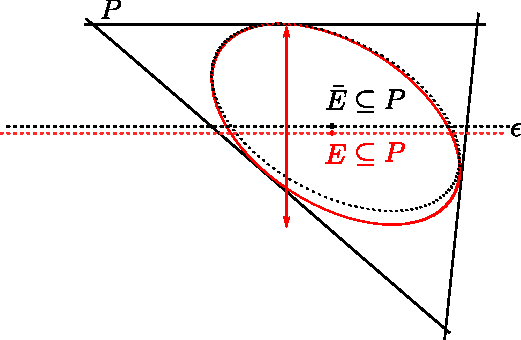
\includegraphics[width=0.65\textwidth]{cutting/fig2}
\par\end{centering}
\caption{Vertical compression of MIE to an approximate MIE}
\end{figure}

\begin{lem}\label{Rate-Decrease2}
The volumes decrease at the rate
\[
\frac{\volmu(P_{k+1})}{\volmu(P_k)}\leq\frac{0.843}{(1-\gamma)^2}
\]
\end{lem}
\begin{proof}
We will split the analysis into two cases. 

% Let $l_k$ be the linear
% lower bound given by the oarcle at iteration $k$
% \[
% l_k(x)=\inf\{t\mid(t,x)\in L_k\}=l_k+g_k^{T}(x-x_k).
% \]
% The two cases are then $l_k(x_k)\leq t_k$, and otherwise.

\noindent\textbf{Case 1: (Deep Cut) $l_k \geq t_k$ or $l_k \leq t_k$ and $u_k \leq t_k$ } 
The intersection of the cutting planes do not contain $(t_k,x_k)$, therefore by Theorem \ref{thm:MIE_cut},
\[
\frac{\volmu(P_{k+1})}{\volmu(P_k)}\leq0.843
\]
\textbf{Case 2: (Shallow Cut) $l_k < t_k$ and $u_k > t_k$}. See Figure \ref{fig:shallow-cut} for an illustration of this case. In this event, our
choice of duality gap ensures that 
\begin{equation}\label{eq:epsilon-bound}
u_k-t_k \leq u_k-l_k\leq \gamma (u^*_k - t_k) \quad \Rightarrow \quad t_k 
+ \gamma (u^*_k - t_k) \geq u_k 
\end{equation}
Consider the ellipse formed by the following compressive transformation
\begin{align*}
\bar{\mathcal{E}} & =\Lambda\left(\mathcal{E}-(u^*_k,0,\dots,0)\right)+(u^*_k,0,\dots,0)\\
\Lambda & =\mbox{diag}([1-\gamma,1,\dots,1]) 
\end{align*}
The center of this compressed ellipse is $(t_k + \gamma(u^*_k - t_k),  x_k)$
which lies at or above $(u_k,  x_k)$, by \eqref{eq:epsilon-bound}. Therefore the horizontal upper bound cuts off the center of $\bar{\mathcal{E}}$. Also observe that
$\bar{\mathcal{E}}\subseteq P$ as $P$ tapers downwards, and the vertical region that lies above  $\mathcal{E}$ is all contained in $P$. Furthermore,
\[
\vol(\bar{\mathcal{E}})=\det(\Lambda)\cdot \vol(\mathcal{E}) =(1-\gamma)\cdot\vol(\mathcal{E})
\]
Therefore, $\bar{\mathcal{E}}$ is a $(1-\gamma)$-approximate ellipsoid, and by
Lemma \ref{lem:approx-MIE-vol}
\[
\frac{\volmu(P_{k+1})}{\volmu(P_k)}\leq\frac{0.843}{(1-\gamma)^2}.
\]
Combining these two cases yields the final result.
\end{proof}
%
Applying this result inductively, we get 
$$
\volmu(P_{k})\leq\left(\frac{0.843}{(1-\gamma)^2}\right)^{k}\volmu(P_{0})
$$

Combining the above two results, we get a final theorem on the convergence rate of our algorithm.
\begin{thm}\label{thm:CG-convergence}
For all $k$ in Algorithm \ref{alg:cutting_plane_epi_err},
\[
u_{k}^{*}-f(x^{*})\leq K\left(\frac{(1-\gamma)^{2}}{0.483}\right)^{k/(n+1)}\quad K=(u_{0}-f(x^{*}))\left(\frac{\volmu(P_{0})}{\volmu(\mathcal{K})}\right)^{1/(n+1)}
\]
and therefore it terminates in no more than
\[
k = \left\lceil \frac{(n+1)\log(K/\mbox{TOL})}{-\log((1-\gamma)^2/\exp(1))} \right\rceil 
\in \mathcal{O}\left(n\log\frac{1}{\mbox{TOL}}\right).
\]
iterations with $$u^*_k - f(x^*) \leq \epsilon$$

\end{thm}

We now show a lower bound on $\epsilon_k$, an analog of Lemma \ref{lem:cg-epsilon-lower-bound}.
% We now focus our attention on the amount of work involved in each
% oracle call. Recall that the cost of invoking the oracle is inversely
% proportional to $\epsilon_k$. Hence we will show a lower bound on $\epsilon_k$
% in the next few lemmas.

% \begin{lem}
% The MIE of $P_k$ always touches the hyperplane $\{(t,x)\mid t=u^*_k\}$
% \end{lem}
% \begin{proof}
% We will show this by contradiction. Consider the case where MIE $\mathcal{E}$
% does not touch the hyperplane $\{(t,x)\mid t=u^*_k\}$. Then consider
% $\mathcal{E}$ stretched, from the bottom of the ellipsoid, till it does touch
% the hyperplane. Since $P_k$ tapers downwards, this new ellipsoid will still be
% a subset of $P$. This new Ellipse will however be strictly larger in volume
% than the original.  This is a contradiction, as  $\mathcal{E}$ is the MIE.
% \end{proof}

\begin{lem}\label{lem:mie-epsilon-lower-bound}
For all $k$,
\[
\epsilon_k\geq \frac{\gamma \, \mbox{\rm height}(P_k)}{n+1}
\]
\end{lem}
\begin{proof}
Since $u^*_k - t_k = \mbox{height}(P_k \cap \{ (t,x) \mid t \geq t_k \})$, we have from Lemma \ref{lem:MIE-1D-Div} and the definition of $\epsilon_k$
\[
\epsilon_k = \gamma \, (u^*_k - t_k) 
\geq\frac{\gamma \, \mbox{height}(P_k)}{n+1}.
\]
% \[
% f(x_k)-[\mbox{center}(\mathcal{E}_k)]_1=\mbox{height}(P\cap\{[t,0,\dots,0]\mid t\geq[\mbox{center}(\mathcal{E}_k)]_1\})
% \].
\end{proof}

Finally, we have the analog of Theorem \ref{thm:cg-total-work}. The result is
identical, apart from constants. The proof of this theorem is identical to that of Theorem $\ref{thm:cg-total-work}$.

\begin{thm}
Define the total amount of work for each oracle call $F(x,\epsilon) = \epsilon^{-1}$. Assume the algorithm is run till termination. Then the total amount of work involved is
\[
\sum{\frac{1}{\epsilon_{k}}}\leq30\cdot\frac{n+1}{\gamma \mbox{TOL}}\left\lceil (n+1)\log\left(\frac{K}{\mbox{TOL}}\right)\right\rceil \in\mathcal{O}\left(\frac{1}{\mbox{TOL}}\log\frac{1}{\mbox{TOL}}\right)
\]
\end{thm}
\begin{proof} From the bound on the total number of iterations, we get
\[
\sum {\frac{1}{\epsilon_k}} 
\leq \frac{n+1}{\gamma\mbox{TOL}}
\left\lceil \frac{(n+1)\log(K/\mbox{TOL})}{-\log((1-\gamma)^2/\exp(1))} \right\rceil
\in \mathcal{O}\left(n\log\frac{1}{\mbox{TOL}}\right).
\]
Optimizing for $\gamma$ numerically, we find that the optimum occurs at $\gamma = 0.41$. Substituting this into the equation, we get the final result.
\end{proof}

% \begin{proof}
% The algorithm terminates when either
% $$
% \mbox{height}(P_k)\leq \epsilon \qquad \mbox{ or }\qquad\volmu(P_k)\leq(\epsilon/K)^{n+1} .
% $$
% Lemma \ref{lem:cg-epsilon-lower-bound} implies the work involved at each
% iteration will be no more than $1/(50(n+1)\epsilon)$. Theorem \ref{thm:MIE-convergence} gives a bound on the total number of iterations. Multiplying the
% two quantities proves the theorem.
% \end{proof}

\section{Strongly Convex Functions}

\begin{algorithm} 
  \SetKwInOut{Input}{input}\SetKwInOut{Output}{output}
  \SetKwProg{Fn}{function}{}{end}
  \SetAlgoNoLine
  \DontPrintSemicolon
  $P_0 = C \times {[\mbox{upper bound on $f$}, \mbox{lower bound on $f$}]}$\;
  
  \While {$\max\{ \mbox{height}(P_k), K \cdot \mbox{size}(P_k)^{1/(n+1)} \} \geq \mbox{TOL}$} {
  \nl $(t_k,x_k) \gets \mbox{\bf center}(P_k)$\;
  \nl $\epsilon_k \gets \gamma (\min \{ u_0, \dots, u_{k-1}\}-t_k )$\;
  \nl $(u_k,l_k,g_k)\gets F(x_k, \epsilon_k )$\;
  \nl $P_{k+1}\gets P_k\cap 
      \underbrace{\{(t,x)\mid t\leq u_k \}}_{\mbox{\tiny upper bound}} \cap 
      \underbrace{\{(t,x)\mid l_k+g_k^{T}(x-x_k)\leq t\}}_{\mbox{\tiny lower bound}}$\;
  \vspace{-5mm}
  \nl $k \gets k+1$  
  }
  \caption{Epigraphical Cutting Plane With Error \label{alg:strongly-convex}}
\end{algorithm}

We can modify our algorithm to exploit additional structure, if available, in the problem. Consider the regularized problem
$$
\mbox{minimize}\quad  f(x) + \tfrac{S}{2}\|x\|^2  \qquad x\in C,
$$
where $f$ is convex, real valued and has a quadratic upper bound at the optimum,
\begin{equation}\label{ass:smooth}
f(x)\leq\tfrac{L}{2}\|x-x^*\|^2+f(x^*).
\end{equation}
The extra regularization parameter allows us to generate parabolic, rather than linear lower bounds on the problem: 
\[
\mbox{for any $x,\epsilon$ } \quad (u,l,g) = F(x,\epsilon),\qquad 
 l+ g^T (\bar{x}-x) +\tfrac{S}{2}\|\bar{x}\|^2 \leq f(\bar{x}) \mbox{ for all }\bar{x}.
\]
It is a simple matter to incorporate these lower bounds in this problem, and
this results in Algorithm \eqref{alg:strongly-convex}. These two modifications will enable us to prove a stronger result on the total
work involved. Indeed, in contrast to the
$\mathcal{O}(\epsilon^{-1}\log\epsilon^{-1})$ amount of work required before,
we now require $\mathcal{O}(\epsilon^{-1})$ work. For simplicity, we will assume that \mbox{\bf{center}} is the center of the MIE, and $\mbox{size}=\mu$ though all the results here can be proven for the CG in a straightfoward manner.

Let us consider why such a regularized system might arise in practice.
First, note that any unregularized, but strongly convex problem can be written
in this form (by adding and subtracting a quadratic term). Therefore this
regularized form of the problem is merely syntactic sugar - we are really
dealing with strongly convex functions. The second assumption of smoothness
holds true if $f$ is smooth and has $L$-Lipshitz gradients. This is true, for
example, if $f$ is a dual of a strongly convex primal problem. (TODO: Try to
work in a reference to Geometric Descent, a similar algorithm which uses
parabolic lower bounds. \cite{drusvyatskiy2016optimal})

In the context of constrained optimization, the regularized problem can be
interpreted as using a squared penalty in lieu  of hard constraints, as the
next example demonstrates.
% \begin{figure}
% \noindent \rule[0.5ex]{1\columnwidth}{0.5pt}
% {Parabolic Inexact Epigraphical Cutting Plane}
% \vspace{-0.5mm}

% \noindent \rule[0.5ex]{1\columnwidth}{0.5pt}

% \begin{algorithmic}
% \State $P_0\supseteq\mbox{epi}(f + \delta_C)$
% \While {$\max\{ \mbox{height}(P_k), \mathcal{O}(1)\cdot n[L^{n}\volmu(P_{k})^2]^{1/(2+n)} \} \geq\epsilon$}
%   \State $(t_k,x_k) \gets \mbox{\bf center}(P_k)$
%   \State $\epsilon_k \gets \tfrac{1}{50}(\min \{ u_0, \dots, u_{k-1}\} - t_k)$  
%   \State $(u_k,l_k,g_k)\gets F(x_k,\epsilon_k) $
%   \State $P_{k+1}\gets P_k\cap 
%       \underbrace{\{(t,x)\mid t\leq u_k \}}_{\mbox{\tiny upper bound}} \cap 
%       \underbrace{\{(t,x)\mid l_k+g_k^{T}(x-x_k) + \tfrac{S}{2}\|x\|^2\leq t\}}_{\mbox{\tiny lower bound}}$
%   \vspace{-4mm}
%   \State $k \gets k + 1$
% \EndWhile
% \end{algorithmic}
% \noindent \rule[0.5ex]{1\columnwidth}{0.5pt}
% \caption{Inexact Epigraphical Cutting plane with parabolic cuts. }\label{alg:strongly-convex}
% \end{figure}

% \noindent \rule[0.5ex]{1\columnwidth}{1pt}
% \begin{enumerate}
%   \item $P_0\supseteq\mbox{epi}(f+\delta_{\mathcal{X}})$
%   \item While $\max\{\mbox{height}(\mathcal{E}_{k}), \mathcal{O}(1)[L^{n}\volmu(P_{k})^2]^{1/(2+n)}\} \geq \epsilon $
%   \begin{enumerate}
%     \item $\mathcal{E}_k=\mbox{maximum volume ellipsoid of \ensuremath{P_k}}$
%     \item $\mbox{center}(\mathcal{E}_k)=(t_k,x_k)$
%     \item $(L_k,U_k)=\mathbf{Oracle}(x_k,\tfrac{1}{50}\mbox{height}(\mathcal{E}_k))$
%     \item $P_{k+1}=P_k\cap U_k\cap L_k$
%   \end{enumerate}
% \end{enumerate}
% \noindent\rule[0.5ex]{1\columnwidth}{1pt}

\begin{example} As noted in the motivation of the introduction, we are interested
in duals of optimization problems with few constraints. Recall the Lagrangian
\[
\mathcal{L}(v,x) = h_0(v) + x_1h_1(v) + \cdots + x_nh_n(v).
\]
Of course, as we have shown, maximizing the variable $x$ over the set $\mathbf{R}_{+}$ will recover
the original constrained problem. Instead of doing that let us regularize
the dual variables with a quadratic term, as shown:
\[
\bar{\mathcal{L}}(x,v)=h_0(v)+x_1h_1(v) + \cdots + x_nh_n(v) - \tfrac{S}{2}\|x\|^2.
\]
Now taking infimums over $v$, we see this is exactly the regularized problem
\[
-\inf_v\bar{\mathcal{L}}(x,v) = f(x) + \tfrac{S}{2}\|x\|^2.
\]
Taking supremums instead over $x$ over $\mathcal{\bar{L}}$, we arrive at an
interpretation for the regularization. We have replaced the hard constraints
with smooth,  quadratic penalties in the objective,
\[
\sup_{x\geq0}\bar{\mathcal{L}}(x,v)=h_0(v)+ \tfrac{1}{S}\big(\max\{0,h_1 (v)^2\} + \cdots + \max\{0,h_n (v)^2\}\big).
\]
If we have upper bounds on the Lagrange multipliers (our variables $x$),
$0\leq x\leq\alpha$, then the quadratic penalties turn into huber penalties. 

% we can maximize $x$ over the
% box to obtain huber penalties on the objective: 
% \[
% \mbox{minimize}\;\; \inf_{\mathclap{0\leq x\leq\alpha}}\,\bar{\mathcal{L}}(x,v)=h_0(v)+
% \tfrac{1}{S} {\textstyle \sum}_i ^{n} \max\{0, \varphi[h_i (v)]\}
% \]
% This relaxation, 
% \[
% \psi(v)=\begin{cases}
% \tfrac{1}{2}v^{2} & |v|\leq \alpha\\
% \alpha[|v|-\tfrac{1}{2}v^{2}] & |v|>\alpha
% \end{cases}
% \]
% therefore, has an interpretation of relaxing the constraints and
% turning them into penalties.
\end{example}

\begin{lem}\label{strongly_convex_upper_bound_obj}
For all $k$,
\[
u^*_k-f(x^*)\leq\mathcal{O}(1)\cdot n[L^{n}\volmu(P_k)^2]^{1/(2+n)}.
\]
where $\mathcal{O}(1)$ is a universal constant.
\end{lem}
\begin{proof}
From Assumption \ref{ass:smooth} we have the following quadratic upper bound
on $f$, 
\[
v:=\tfrac{L}{2}\|\cdot-x^*\|^2+f(x^*),
\]
i.e. $v \geq f$. Define the two sets $\mathcal{K}_k$, $\mathcal{P}_k$ for which 
$\mathcal{K}_k \subseteq \mathcal{P}_k \subseteq P_k$,
\begin{equation*}
  \mathcal{K}_k  =\mbox{conv}\{u^*_k\times\mbox{lvl}(v,u^*_k),(f(x^*),x^*)\}.
  \quad
  \mathcal{P}_k  =\mbox{epi}(v)\cap\{(t,x)\mid t\leq u^*_k\},
\end{equation*}
Also, let $\mathcal{K}$ be a unit circular cone
\[
\mathcal{K}=\mbox{conv}\big\{\{(1,x)\mid \tfrac{1}{2}\|x\|^2\leq1\},0\big\}.
\]
% The epigraph of our upper bound
% \[
% \mbox{epi}(v-f(x^*))-x^*=\{x\mid\tfrac{1}{2}\|x\|^2\leq([u_k-f(x^*)]/L)^{1/2}\}
% \]
First note that $\mathcal{K}_k$ and $\mathcal{K}$, our standard cone, are related
by a affine transformation. This transform which first involves the translation of the tip of the cones to $(0,0)$, and then a scaling.
\begin{align}\label{eq:translate_standard_cone}
\mathcal{K} & =\Sigma^{-1}_k(\mathcal{K}_k-(f(x^*),x^*))\\
\Sigma_k & =\mbox{diag}([u_k-f(x^*),([u_k-f(x^*)]/L)^{1/2},\dots,([u_k-f(x^*)/L])^{1/2})
\end{align}
Therefore, the following chain of inequalities follow:
\begin{align*}
\volmu(P_k) & \overset{(a)}{\geq}\volmu(\mathcal{P}_k) \\
& \overset{(b)}{\geq}\volmu(\mathcal{\mathcal{K}}_k) 
 \overset{(c)}{=}\det(\Sigma_k)\volmu(\mathcal{K})  
=\volmu(\mathcal{K})[u_k-f(x^*)]^{(2+n)/2}/L^{n/2}
\end{align*}
$(a)$ comes from Assumption \eqref{ass:smooth}, which implies $P_k \subseteq \mathcal{P}_k$.
$(b)$ follows from the fact that $\mathcal{P}_k\supseteq\mathcal{K}_k$,
by construction ($\mathcal{K}_k$ is a circular cone inscribed in the parabola
$\mathcal{P}_k$.)
$(c)$ comes from translating and scaling $\mathcal{K}_k$ into the standard cone, equation \eqref{eq:translate_standard_cone},  the affine invariance of the MIE, and the affine homogeneity of $\volmu$. Taking powers of $2/(2+n)$ on both sides, we get the final result
\[
u^*_k-f(x^*)
\leq\frac{L^{n/(2+n)} \volmu(P_k)^{2/(2+n)}}{\volmu(\mathcal{K})^{2/(2+n)}}
\leq\mathcal{O}(1)\cdot n[L^n\volmu(P_k)^2]^{1/(2+n)}.
\]
For the final inequality, we use the fact that 
$$\volmu(\mathcal{K})^{2/(2+n)}\geq \frac{\omega_{n}^{2/(2+n)}}{4^{\frac{2n+2}{2+n}}}\geq n \mathcal{O}(1)$$ 
for all $n$.
\end{proof}

This theorem can be seen as a quadratic improvement over Lemma
\ref{lem:lem-voldecrease}. In Lemma
\ref{lem:lem-voldecrease} we proved $ u^*_k-f(x^*)
\lessapprox \volmu(P_k)^{1/(n+1)}. $ This theorem improves that bound to $
u^*_k-f(x^*) \lessapprox \volmu(P_k)^{2/(2+n)}. $ This fact allows us to relax the
termination condition by a squared factor.  Note too, that this improvement
does not depend on the parabolic cutting  planes, and hence can be integrated
with the results in the previous section. This results in 

\begin{thm}\label{thm:MIE-convergence-2}
% For all $k$
% \[
% u^*_k-f(x^*)\leq (0.878)^{k/(n+1)}\cdot K\volmu(P_0)^{1/(n+1)}
% \]
% and when 
Algorithm \ref{alg:cutting_plane_epi_err} terminates in no more than
\[
k = \left\lceil \frac{(2+n)\log(1/\epsilon)+2\log\volmu(P_{0})+n\log L}{\log(1/0.878^{2})} \right\rceil
\in \mathcal{O}\left(n\log\frac{1}{\epsilon}\right)
\]
iterations. When Algorithm \ref{alg:strongly-convex} terminates,
\[
u^*_k - f(x^*) \leq \epsilon
\]
\end{thm}

The improvement above is not significant, and does not change the algorithms
complexity class. The above statement merely establishes that this new
stopping criteria is valid. The next theorem establishes a lower bound on
$\epsilon_k$ as a function of $\volmu(P_k)$. The parabolic lower bounds,
intuitively, prevent $P_k$ from becoming too flat.

\begin{figure}
\begin{centering}
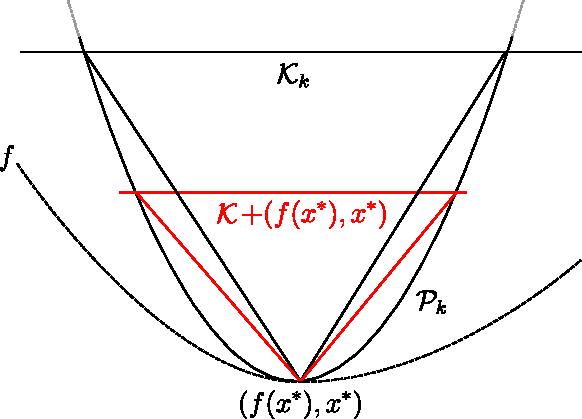
\includegraphics[width=0.65\textwidth]{cutting/fig5}
\par\end{centering}
\caption{Illustration of inner approximating cones, and the rescaling by $\Sigma_k$ necessary to transform it into the unit cone.}
\end{figure}

\begin{lem}\label{lem:strongly_convex_lower_bound_k}
For all $k$
\[
\epsilon_k\geq\mathcal{O}(1)\cdot[S{}^{n}\volmu(P_k)^2]^{1/(2+n)}
\]
Where $\mathcal{O}(1)$ is a universal constant.
\end{lem}
\begin{proof}
Let $l^*_k$ be the strongest lower bound at iteration $k$,
\[
l^*_k = \max_{i < k}\{l_i + g_i^T(\cdot-x_i) + \tfrac{S}{2}\|\cdot \|^2\}.
\]
Since each function within the $\max$ is strongly convex with modulus $S$,
so must $l^*_k$ (strong convexity is preserved by the $\max$). Let $\hat{x}^*$ be the minimizer of $l^*_k$. Since $0\in\partial l^*_k(\hat{x}^*)$ (see Figure \ref{fig:parabolic_outer_approximation}),
\[
l^*_k(x)\geq l^*_k(\hat{x}^*)+0^{T}(x-\hat{x}^*)+\tfrac{S}{2}\|x-\hat{x}^*\|^2\geq l^*_k(\hat{x}^*)+\tfrac{S}{2}\|x-\hat{x}^*\|^2,
\]
This implies $\mbox{epi}(l^*_k) \subseteq\mbox{epi}(l^*_k(\hat{x}^*)+\tfrac{S}{2}\|\cdot-\hat{x}^*\|^2)$ and therefore
\begin{align}\label{eq:subset_P_k_Parabola_k}
P_k & =\mbox{epi}(l^*_k) \cap \{(t,x) \mid t \leq u^*_k \} \\
    & \subseteq\mbox{epi}(l^*_k(\hat{x}^*)+\tfrac{S}{2}\|\cdot-\hat{x}^*\|^2)\cap \{(t,x) \mid t \leq u^*_k \}  =:\mathcal{P}_k
\end{align}
See Figure \ref{fig:parabolic_outer_approximation} for an illustration. Lete $\omega_n$ be the volume of a unit $n$-ball.
\begin{align*}
\volmu(P_k) & \overset{(a)}{\leq}\vol(P_k)\\
 & \overset{(b)}{\leq}\vol(\mathcal{P}_k) \\
 & \overset{(c)}{=}\frac{2\omega_n}{n[S/2]^{n/2}}\cdot \mbox{height}(\mathcal{P}_k)^{(2+n)/2} \\
 & \overset{(d)}{=}\frac{2\omega_n}{n[S/2]^{n/2}}\cdot \mbox{height}(P_k)^{(2+n)/2} \\
 & \overset{(e)}{\leq}\frac{2\omega_n }{n[S/2]^{n/2}} \cdot [(n+1)\epsilon_k]^{(2+n)/2}
\end{align*}
$(a)$ comes from the fact that $\volmu(P_k)=\vol(\mathcal{E}_k),$
and $\mathcal{E}_k$, being an inscribed ellipse, is a subset of
$P_k$. $(b)$ comes from \eqref{eq:subset_P_k_Parabola_k}. Finally, $(c)$ is the volume
of a parabola. $(c)$ is from construction (see Figure \ref{fig:parabolic_outer_approximation}), and $(d)$ comes from Lemma \ref{lem:MIE-1D-Div}. Taking powers of
$2/(2+n)$ on both sides, we obtain
% \[
% \epsilon_k\geq\frac{[S/2]^{n/(2+n)}}{(n+1)[n\omega_n]{}^{2/(2+n)}}\cdot\volmu(P_k)^{2/(2+n)}\geq\mathcal{O}(1)\cdot[S{}^{n}\volmu(P_k)^2]^{1/(2+n)}
% \]
\[
\epsilon_k \geq \frac{n^{2/(2+n)}}{2}\cdot \frac{[\volmu(P_{k})^{2}S^{n}]^{1/(2+n)}}{(n+1)[\omega_{n}]^{2/(2+n)}}
\geq \mathcal{O}(1)\cdot[S{}^{n}\volmu(P_k)^2]^{1/(2+n)}
\]
The final inequality comes from the Lemma \ref{vol-sphere-bound}.
% (i haven't proved the last part formally, 
% but an informal proof goes along the lines of $\omega_n^{-2/(2+n)} \in \mathcal{O}(n)$
% and so the terms should multiply to give a constant. The quantity above seems to be bounded by 18. This conjecture holds in wolfram alpha too.)
% type {\tt plot (pi^(n/2)/gamma(n/2+1))^(-2/(2+n)) for  0< n < 100} and {\tt plot (n+1)*(pi^(n/2)/gamma(1+n/2))^(2/(n+2)) for 0 < n < 300)} into wolfram alpha for plots)
\end{proof}

\begin{figure}
\begin{centering}
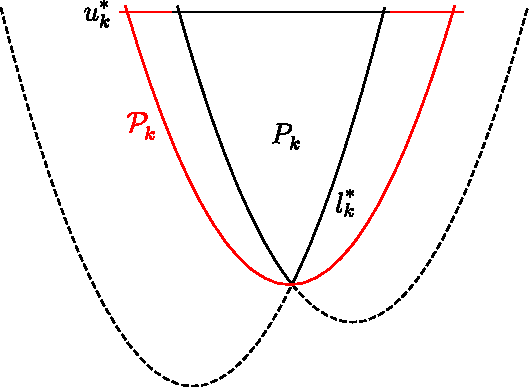
\includegraphics[width=0.65\textwidth]{cutting/fig4}
\par\end{centering}
\caption{Geometric Illustration of the parabolic outer approximation
of $P_k$, i.e. $P_k \subseteq \mathcal{P}_k$. \label{fig:parabolic_outer_approximation}}
\end{figure}


Finally, we bound the total amount of work involved in the algorithm. We assume that the amount of work is inversely proportional to $\epsilon$. 

\begin{thm}
Assume the algorithm is run till termination. Then for $\epsilon>0$
\[
\sum\frac{1}{\epsilon_k}\leq\frac{L}{S}\cdot\frac{\mathcal{O}(1)}{1-0.878^{2/(2+n)}}\cdot\frac{n}{\epsilon}
\]
Where $\mathcal{O}(1)$ represents a universal constant.
\end{thm}
\begin{proof}
Let $\volmu_k:=\volmu(P_k)^{2/(2+n)}.$ Then we have the following three
guarantees. 
\begin{alignat*}{2}
  \epsilon_k & \geq C_1\volmu_k &  & \mbox{(Lower bound on $\epsilon_k$, Lemma \ref{lem:strongly_convex_lower_bound_k})}\\
  \volmu_k & \geq C_2\epsilon & \qquad & \mbox{(Termination criteria, Algorithm \ref{alg:strongly-convex})}\\
  \volmu_k & \geq0.878^{-2/(2+n)}\cdot\volmu_{k+1} &  & \mbox{(Convergence guarantee, Lemma \ref{Rate-Decrease2})}
\end{alignat*}
where
\[
C_1=\mathcal{O}(1)\cdot S^{n/(2+n)},\qquad C_2=\mathcal{O}(1)\cdot L^{-n/(2+n)}
\]
Therefore, the total cost of the iteration is 
\[
\sum\frac{1}{\epsilon_k}\leq\sup\{\alpha_0,\alpha_1,\dots\},
\]
where $\alpha_j$ is the total amount of work performed if the algorithm
ran for $j$ steps. We can upper bound the total amount of work performed 
by performing an optimization over the three constraints described above.
Let $\beta=0.878^{-2/(2+n)}.$ Then 
\begin{align*}
\alpha_{j} 
  & \leq \sup\,\{\,{\textstyle \sum_{k=0}^j}\epsilon_k^{-1}\mid\volmu_0\geq\beta\volmu_1,\cdots,\volmu_{j-1}\geq\beta\volmu_{j}\mbox{ and }\volmu_k\geq C_2\epsilon,\epsilon_k\geq C_1\volmu_k\mbox{, $\forall k$}\}\\
  & =\sup\,\{\,{\textstyle \sum_{k=0}^j}\,\epsilon_k^{-1}\mid\volmu_0\geq\beta\volmu_1,\cdots,\volmu_{j-1}\geq\beta\volmu_{j}\mbox{ and }\volmu_k\geq C_2\epsilon,\epsilon_k=C_1\volmu_k\mbox{, $\forall k$}\}\\
  & =\sup\,\{\,{\textstyle \sum_{k=0}^j}\,[C_1\volmu_k]^{-1}\mid\volmu_0\geq\beta\volmu_1,\cdots,\volmu_{j-1}\geq\beta\volmu_{j},\volmu_j\geq C_2\epsilon\}\\
  & \overset{(1)}{=}\frac{{\textstyle \sum_{k=0}^j}\beta^{-k}}{C_1C_2\epsilon}
  \leq \frac{{\textstyle \sum_{k=0}^{\infty}}\beta^{-k} } { C_1C_2\epsilon}
  =\frac{1}{( 1-{\beta^{-1}} )C_1C_2\epsilon } 
\end{align*}
Inequality $(1)$ comes from Lemma \ref{lem:maximization_convex}. Our objective function
is convex, and bounded from above on the feasible set (the function is decreasing, and the feasible set does not contain $0$). By writing the constraints as
$$ 
\left(\begin{array}{cccc}
1 & -\beta\\
 & \ddots & \ddots\\
 &  & 1 & -\beta\\
 &  &  & 1
\end{array}\right)\left(\begin{array}{c}
\volmu_{0}\\
\vdots\\
\volmu_{j-1}\\
\volmu_{j}
\end{array}\right)\geq\left(\begin{array}{c}
0\\
\vdots\\
0\\
C_2\epsilon
\end{array}\right).
$$
The statement of the lemma states that the optimum is achieved at equality. Therefore the optimum is achieved at $\volmu_{k}=\beta^{j-k}C_2\epsilon$. Substituting this back into the objective and reversing the order of summation yields the equality. Finally,
\[
\frac{1}{C_1C_2}=
\frac{\mathcal{O}(1)\cdot n L^{n/(2+n)}}{\mathcal{O}(1)\cdot S^{n/(2+n)}} 
\leq\mathcal{O}(1)\cdot\frac{n L}{S}
\]
as $L/S \geq 1$ which implies $(L/S)^p
\leq L/S$ for $p\leq1$
\end{proof}
%

Surprisingly, there are no constants in the above proof which involve
$\volmu(P_0)$. This counterintuitive fact means the volume of the initial
localization polytope plays no role in the optimization. How can this be
possible?  Perhaps this can be understood with the following intuition. Since
the iterates at the beginning get exponentially cheaper as the polytope $P_0$
increases, in a sense, early iterations contribute very little to the work
involved. In practice, of course, this is not the case. There is some, finite
fixed cost in solving any optimization problem, which cannot be atomically
divided. However we believe that this property still translates to much better
performance in practice.

\section{Some General Facts}
\begin{lem} \label{vol-paranolid}
({\bf Volume of a Parabolid}) Let $\omega_n$ be the volume of the $n$ unit ball. Then
\[
{\rm vol}(\{(t,x)\mid\tfrac{K}{2}\|x\|^2\leq t \leq h\})=
\frac{2\omega_n}{n[K/2]^{n/2}}\cdot h^{(2+n)/2}.
\]
\end{lem}
\begin{proof}
This proof is an application of the ``disk method'' in calculus.
Since
\[
\frac{K}{2}\|x\|^2\leq t\iff\|x\|\leq\sqrt{2t/K},
\]
each slice of $\mathcal{P}$ in the first dimension is a $n-$ball
of radius $\sqrt{2t/K}$, with area $\omega_n(2t/K)^{n/2}$. We integrate
this from $0$ to $h$,
i.e.,
\[
{\rm vol}(\mathcal{P})=
\omega_n\int_0^{h}[2t/K]{}^{n/2}dt=
\frac{\omega_n}{[K/2]^{n/2}}\int_0^{h}t^{n/2}dt=
\frac{2\omega_n}{n[K/2]^{n/2}}\cdot h^{(n+2)/2}.
\]
\end{proof}
%

\begin{lem} (Volume approximations for MIE of the unit circular cone)
Let 
$$\mathcal{K} = \mbox{\normalfont conv}\big\{\{(1,x)\mid \tfrac{1}{2}\|x\|^2\leq1\},0\big\}.$$ Then $$ \frac{\omega_{n+1}}{4^{n+1}} \leq \volmu({\mathcal{K}}) \leq \frac{2^{n/2+1}\omega_{n}}{n}$$
\end{lem}
\begin{proof} {(\bf{Lower Bound})} We can inscribe a $n+1$ dimensional ball of radius $1/(2\sqrt{1.25} + 1)$ in the unit cone. Since the MIE is larger than this,
$$\frac{\omega_{n+1}}{(2\sqrt{1.25}+1)^{n+1}} \leq \volmu(\mathcal{K}).$$
{(\bf{Upper Bound})} Since $\volmu(\mathcal{K}) \leq \mbox{vol}(\mathcal{K})$, we can use Lemma \ref{vol-paranolid}
\end{proof}

\begin{lem}\label{lem:maximization_convex}
({\bf Maximization of a convex function over a cone}) Let $f$ be
a convex function, and $A$ be a square, invertible matrix. Furthermore assume that $f$ is bounded on the
cone $\{x\mid Ax\geq b\}$. Then 
\[
\sup_{x}\,\{f(x)\mid Ax\geq b\} = f(A^{-1}b).
\]
\end{lem}
\begin{proof}
We transform the problem to 
\[
\sup_{x}\,\{f(x)\mid Ax\geq b\}=\sup_{x}\,\{f(A^{-1}(x+b))\mid x\geq0\}=\sup_{x}\{g(x)\mid x\geq0\}
\]
Where $g(x)=f(A^{-1}(x+b))$. By assumption, the function $g$ is bounded, and
therefore is decreasing on every half line \cite{Roc70}, and achieves the
maximum at $g(0)$. Therefore, $g$ must attain a global minimum at $g(0)=f(A^{-1}b)$.
\end{proof}

\begin{lem}\label{lem:MIE-1D-Div}
Let $P\subseteq R^{n+1}$ be a compact polytope, and assume that the
center of the maximum volume elipsoid of $P$ is $a$. Then
\[ 
\frac{1}{n+1}\leq
\frac{\mbox{\rm height}
(\ensuremath{P\cap \{(t,x)\mid t\geq a_1\})}}{\mbox{\rm height(\ensuremath{P})}}
\leq\frac{n}{n+1}
\]
\end{lem}
\begin{proof}
Let $\mathcal{E}$ be the MIE of $P$. Assume, w.l.o.g, $\mathcal{E}$ is centered at $0$. By \cite{tarasov1988method} we know that
\[
\mathcal{E}\subseteq P\subseteq n \mathcal{E}
\]
Define the $\mbox{Proj}$ to be the projection of the set $P$ onto
the first coordinate,
\[
\mbox{Proj}(P)=\{t\mid(t,\bar{x})\in P\mbox{\}}
\]
Since $\mathcal{E},P,n \mathcal{E}$ are all convex, their corrosponding projections are
intervals. Since $\mathcal{E},n \mathcal{E}$ are both ellipses centered at $0$, we can
assume then without loss of generality (since the ratios are preserved)
\[
\mbox{Proj}(\mathcal{E}):=[-1,1],\quad\mbox{Proj}(P):=[-x_1,x_2],\quad\mbox{Proj}(n \mathcal{E}):=[-n,n]
\]
Using the fact that 
\[
\mbox{Proj}(\mathcal{E})\subseteq\mbox{Proj}(P)\subseteq\mbox{Proj}(n \mathcal{E})
\]
we have
\[
[-1,1]\subseteq[-x_1,x_2]\subseteq[-n,n]
\]
Then for $H = \{(t,x)\mid t\geq a_1\})$
\[
\frac{\mbox{height(\ensuremath{P\cap H)} }}{\mbox{height(\ensuremath{P})}}=\frac{x_1}{x_2+x_1}\leq\sup\left\{ \frac{x_1}{x_2+x_1}\,\Big|\;\begin{array}{c}
1\leq x_1\leq n\\
1\leq x_2\leq n
\end{array}\right\} =\frac{n}{n+1}
\]
The final equality can be found by solving a simple $2d$ optimization
problem over a box, for which we can exhaustively search all critical
points. Replacing the $\sup$ with an $\inf$, we obtain the other bound.
\end{proof}

\begin{figure}
\begin{centering}
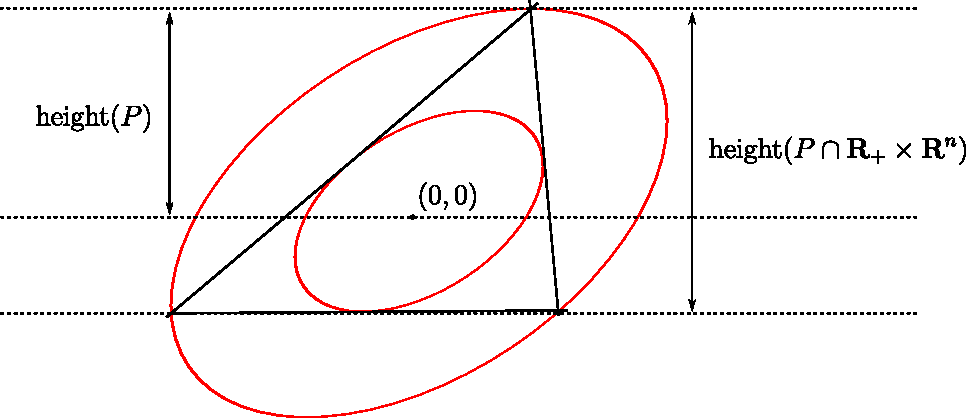
\includegraphics[width=0.65\textwidth]{cutting/fig1}
\par\end{centering}
\caption{Case where lower bound is tight in $2d$. The $n-$dimensional simplex
achieves this bound in general.}

\end{figure}

\begin{lem} \label{vol-sphere-bound}
Let $\omega_n$ be the volume of a unit sphere. Then

$$ \frac{2}{n+1} \leq \omega_{n}^{2/(2+n)}\leq \frac{12}{n+1}$$
\end{lem}
\begin{proof} Multiplying both sides by $n+1$, we get
\begin{align*}
(n+1)\omega_{n}^{2/(2+n)} & =(n+1)\left(\frac{\pi^{\frac{n}{2}}}{\Gamma(\frac{n}{2}+1)}\right)^{2/(2+n)}\\
 & \overset{(a)}{\leq}(n+1)\left(\frac{\pi^{\frac{n}{2}}}{\sqrt{2\pi}n^{\frac{n+3}{2}}e^{-\frac{n+2}{2}}}\right)^{2/(2+n)}\\
 & =(n+1)\frac{\pi^{\frac{n}{2+n}}}{\sqrt{2\pi}n^{\frac{n+3}{n+2}}e^{-1}}\\
 & =\frac{n+1}{n^{1+\frac{1}{n+2}}}\frac{\pi^{\frac{n}{2+n}}}{\sqrt{2\pi}e^{-1}}\\
 & \leq\left(1+\frac{1}{n}\right)\frac{3\pi e}{\sqrt{2\pi}}
  \leq\frac{6\pi e}{\sqrt{2\pi}} \leq 12
\end{align*}
$(a)$ comes from sterling's lower bound. The lower bound is proved in an analogous way
\begin{align*}
(n+1)\omega_{n}^{2/(2+n)} & =(n+1)\left(\frac{\pi^{\frac{n}{2}}}{\Gamma(\frac{n}{2}+1)}\right)^{2/(2+n)}\\
 & \geq(n+1)\left(\frac{\pi^{\frac{n}{2}}}{\sqrt{2\pi}\cdot n^{n+\frac{1}{2}}e^{\frac{1}{12n}-n}}\right)^{2/(2+n)}\\
 & =(n+1)\frac{\pi^{\frac{n}{2+n}}}{\sqrt{2\pi}\cdot n^{\frac{n+3}{2+n}}e^{\left(\frac{2}{2+n}\right)\left(\frac{1}{12n}-n\right)}}\\
 & \geq\frac{n+1}{n}\frac{10}{\sqrt{2\pi}}
\end{align*}
\end{proof}


   \chapter[Proximal Gradient With Error]{ Proximal Gradient With Error }
   \label{ch:ProximalGradientError}
   %!TEX root = ../Dissertation.tex

We will assume for simplicity that
$\alpha_{k}\equiv 1/L$. We will make the following blanket
assumptions about $f$. First, the solution set $\Soln$ of \eqref{eq:minimize_fpg}
is nonempty. For all $x$ and $y$, there exist  positive constants $L$
and $\tau\geq 1$ such that
\begin{subequations}
\begin{align}
  \|{\nabla f(y)-\nabla f(x) \|} 
  &\le L\,\|{y-x}\|, 
  \label{a:lipschitz}
  \\ \min_{\bar{x}\in\Soln}\,\|x-\bar{x}\|
  &\leq\tau\,\|{x-\mathbf{prox}_{1/L}(x-\tfrac1L\nabla f(x)})\|\qquad 
  \forall x \in \mbox{dom}(g)
   \label{a:natural-res}
\end{align}
\end{subequations}
Assumption~\eqref{a:lipschitz} asserts the Lipschitz continuity of the
gradient of $f$. Assumption~\eqref{a:natural-res} is an error bound on
the generalized residual. This generalized residual has been explored
in local contexts in Tseng and Yun~\cite{Tsy09a} and Luo and
Tseng~\cite{LuT94}; for simplicity our assumption is stronger,
however, requiring the bound to be global.

$\tau$ can be seen as a nonsmooth proxy for the condition number. If
$g\equiv0$ and $f$ is strongly convex with parameter $\mu$, then
\eqref{a:natural-res} holds with $\tau = L/\mu$. More generally, if
$g$ is an indicator function on a polyhedral set and $f$ is strongly
convex, this bound holds globally, with parameter $\tau = (L +
1)/\mu$. \cite{Pan87} Theorem 3.1. Recently, a global version of this
error bound has been developed for non- strongly convex functions
which degrades with the size of the neighborhood see
\cite{wang2014iteration} Theorem 18. We can use such a bound if the
function $g$ is an indicator over a polyhedral set, and $f$ can be
written in the form \[ f(x) = r(Ax) + b^{T}x \] for any $A$, $b$,
and $r$ is strongly convex. If the above two conditions hold, then

% Let $R^k:=\sum_{i=0}^{k-1}\rho^i$, where $\rho<1$ is a constant
% specified in Lemma~\ref{lem:obj-val-bnd} in terms of $L$ and $\tau$.
% Let $\mathcal{F}_k=\sigma(e_1,e_2,\ldots,e_k)$ be the $\sigma$-algebra
% generated by the sequence of errors $e_{i}$. When the context is
% clear, $[z]_{i}$ denotes the $i$th component of a vector~$z$.

\begin{lem}
  \label{lem:obj-val-bnd}
  Let $\pi_k = f(x_k) - \min f(x)$. Then after $k$ iterations of algorithm~\eqref{eq:prox-gradient},
  \begin{equation*}
    \pi_k  \le \rho^k \pi_0 
    + \frac{1}{\vartheta}
    \sum_{i=0}^{k-1}\rho^{k-1-i}\|e_i\|^2,
  \end{equation*}
  where
  $$\rho = 1- \frac{1}{1+40\tau^{2}}\in(0,1) \qquad \text{and} 
  \qquad \vartheta = L\cdot\left(\frac{1}{40\tau^{2}}+1\right)>0.$$
\end{lem}

The proof of this result follows the template laid out by Luo and
Tseng \cite[Theorem~3.1]{luo1993error}, modified to keep the error
term $e_k$ explicit. So~\cite{So:2013} also provides a similar
derivation for the case where $g\equiv0$, in which case it seems
possible to obtain tighter constants $\rho$ and $\vartheta$.  If
additionally $\|e_{k}\|=0$, then the result reduces to the well-known
fact that steepest descent decreases the objective value linearly. The
convergence rate, as expected, is a function of the condition number,
We
note that the constants are invariant to scalings of $f+g$.

\noindent 
\begin{lem}[\bf Three-point property with error] \label{le:3-points}
For all $y\in \text{dom}(g)$,
\begin{align*}
  g(y) &\geq g(x_{k+1})
  +{(\nabla f(x_{k})+e_{k})}^T{x_{k+1}-y}
 +\frac{L}{2}\|x_{k+1}-x_{k}\|^{2}
 +\frac{L}{2}\|y-x_{k+1}\|^{2}-\frac{L}{2}\|y-x_{k}\|^{2}.
\end{align*}
\end{lem}

\begin{proof}
Let $\psi_{k}(x) := g(x)+f(x_{k})+\left\langle \nabla
  f(x_{k})+e_{k},x-x_{k}\right\rangle +\frac{L}{2}\|x-x_{k}\|^{2}$. 
Because $\psi_{k}$ is strongly convex,
\[
  \psi_{k}(y)\geq\psi_{k}(x)
  + {q^T}{y-x}
  + \frac{L}{2}\|y-x\|^{2}
  \quad\mbox{for all $x,y$ and all $q\in\partial\psi_k(x)$.}
\]
Choose $x=x_{k+1}:=\text{argmin}\,\phi_{k}(x)$. Because
$0\in\partial\psi_k(x_{k+1})$, we have
$$\psi_{k}(y)\geq\psi_{k}(x_{k+1})+\frac{L}{2}\|y-x_{k+1}\|^{2},$$
which, after simplifying, yields the required result.
\end{proof}


\begin{lem}\label{lem:fourbounds} Let $\bar{x}_k$ be the projection 
of $x_k$ onto $\Soln$. Then
\begin{subequations}
\begin{align} 
  \|x_{k}-\bar{x}_k\|^{\phantom2}
  &\leq\tau\|x_{k}-x_{k+1}\|+\frac{\tau}{L}\|e_{k}\|;
  \label{eq:a1a}
\\ \|x_{k}-\bar{x}_k\|^{2} 
  &\leq2\tau^{2}\|x_{k}-x_{k+1}\|^{2}
  +\frac{5}{4}(\tau^{2}/L^{2})\|e_{k}\|^{2};
  \label{eq:a1b}
\\ \|x_{k+1}-\bar{x}_k\|^{\phantom2} 
  & \leq(1+\tau)\|x_{k}-x_{k+1}\|+\frac{\tau}{L}\|e_{k}\|;
  \label{eq:a1c}
\\ \|x_{k+1}-\bar{x}_k\|^{2} & 
  \leq\frac{1}{2}[2+5\tau+3\tau^{2}]\|x_{k}-x_{k+1}\|^{2}
  +\tfrac{1}{2L^{2}}[3\tau^{2}+\tau]\|e_{k}\|^{2}.
  \label{eq:a1d}
\end{align}
\end{subequations}
\end{lem}
\begin{proof}
 For all $k$,
\begin{align*}
\|x_{k}-\bar{x}_k\|
  &\overset{(i)}{\leq}\tau\|x_{k}
  - [x_{k}-\tfrac{1}{L}\nabla f(x_{k})]_{+}\|
\\&\leq
    \tau \|x_{k}-x_{k+1}\|
  + \tau \|x_{k+1}
  - [x_{k}-\tfrac{1}{L}\nabla f(x_{k})]_{+}\|
\\&=\tau \|x_{k}-x_{k+1}\|
  + \tau \|[x_{k}-\tfrac{1}{L}(\nabla f(x)+e_{k})]_{+}
          -[x_{k}-\tfrac{1}{L}\nabla f(x_{k})]_{+}\|
\\& \overset{(ii)}{\leq}\tau\|x_{k}-x_{k+1}\|+\tfrac{\tau}{L}\|e_{k}\|,
\end{align*}
where $(i)$ follows from Assumption~\eqref{a:natural-res} and $(ii)$
follows from the nonexpansiveness of the proximal operator.

\paragraph{\bf Part \eqref{eq:a1b}}Square both sides of~\eqref{eq:a1a}
and then apply the inequality
\begin{equation}\label{eq:crossterm}
ab\leq\frac{a^{2}}{2\alpha}+\frac{\alpha b^{2}}{2},
\quad \forall\alpha>0,
\end{equation}
to bound the cross terms:
\begin{align*}
  \|x_{k}-\bar{x}_k\|^{2}
  & \leq\tau^{2}\|x_{k}-x_{k+1}\|^{2}
  +(\tau/L)^{2}\|e_{k}\|^{2}+(\tau^{2}/L)\|x_{k}-x_{k+1}\|\|e_{k}\|
\\& \leq\big(\tau^{2}
  +\tfrac{\tau^{2}\alpha}{2L}\big)\|x_{k}-x_{k+1}\|^{2}
  +\big(\tfrac{\tau^{2}}{L^{2}}
  +\tfrac{\tau^{2}}{2L\alpha}\big)\|e_{k}\|^{2}\qquad(\forall\alpha>0)
\\& \leq2\tau^{2}\|x_{k}-x_{k+1}\|^{2}
  +\tfrac{5}{4}(\tau^{2}/L^{2})\|e_{k}\|^{2}.
\end{align*}

\paragraph{\bf Part \eqref{eq:a1c}} Use the triangle inequality
and~\eqref{eq:a1a}:
\[
  \|x_{k+1}-\bar{x}_k\|
  \leq\|x_{k+1}-x_{k}\|+\|x_{k}-\bar{x}_k\|
  \leq(1+\tau)\|x_{k}-x_{k+1}\|+(\tau/L)\|e_{k}\|.
\]

\paragraph{\bf Part \eqref{eq:a1d}} Square both sides above, and use the
same technique used in Part~\eqref{eq:a1b} to bound the cross-terms:
\[
  \|x_{k+1}-\bar{x}_k\|^{2}
  \leq\tfrac{1}{2}(2+5\tau+3\tau^{2})\|x_{k}
  -x_{k+1}\|^{2}+\tfrac{1}{2L^{2}}(3\tau^{2}+\tau)\|e_{k}\|^{2}.
\]
\end{proof}

\begin{lem}[Sufficient decrease] 
\label{lem:sufficient_decrease} For all $k$, 
\[
\pi_{k+1}\leq\left(1-\frac{1}{1+40\tau^{2}}\right)\pi_{k}
   +\frac{1}{L}\cdot\frac{40\tau^{2}}{1+40\tau^{2}}\|e_{k}\|^{2}.
\]
\end{lem}

\begin{proof} First, specialize Lemma~\ref{le:3-points} with $y=x_{k}$:
\begin{equation} \label{eq:3pta}
g(x_{k+1}) \leq g(x_{k})-\left\langle \nabla f(x_{k})
  +e_{k},x_{k+1}-x_{k}\right\rangle -L\|x_{k+1}-x_{k}\|^{2}.
\end{equation}
Then,
\begin{align*}
h(x_{k+1}) & \overset{(i)}{\leq}f(x_{k})+\left\langle \nabla f(x_{k}),x_{k+1}-x_{k}\right\rangle +\frac{L}{2}\|x_{k+1}-x_{k}\|^{2}+g(x_{k+1})\\
 & \overset{(ii)}{\leq}f(x_{k})+\left\langle \nabla f(x_{k}),x_{k+1}-x_{k}\right\rangle +\frac{L}{2}\|x_{k+1}-x_{k}\|^{2}+g(x_{k})\\
 &\qquad-\left\langle \nabla f(x_{k})+e_{k},x_{k+1}-x_{k}\right\rangle -L\|x_{k+1}-x_{k}\|^{2}\\
 &= h(x_{k})-\left\langle e_{k},x_{k+1}-x_{k}\right\rangle -\frac{L}{2}\|x_{k}-x_{k+1}\|^{2}\\
 &\leq h(x_{k})+\tfrac{1}{2\alpha}\|e_{k}\|^{2}+\Big(\frac{\alpha}{2}-\frac{L}{2}\Big)\|x_{k}-x_{k+1}\|^{2},
\end{align*}
where $(i)$ uses Assumption~\eqref{a:lipschitz} and $(ii)$ uses
the~\eqref{eq:3pta}. Choose $\alpha=L/2$ and rearrange terms to obtain
the required result.
\end{proof}

We now proceed with the proof of Lemma~\ref{lem:obj-val-bnd}.  Let
$\bar{x}_k$ be the projection of $x_k$ onto the solution set
$\Soln$. By the mean value theorem,
\begin{equation} \label{eq:eq_mv}
  f(x_{k+1})-f(\bar{x}_k)
  = \left\langle \nabla f(\xi),x_{k+1}-\bar{x}_k\right\rangle.
\end{equation}
From Lemma~\ref{le:3-points}, we have
\begin{align} \label{eq:eq_3pt1}
g(x_{k+1})-g(\bar{x}_k) 
& \leq-\left\langle \nabla f(x_{k})
  +e_{k},x_{k+1}-\bar{x}_k\right\rangle \nonumber 
  -\frac{L}{2}\|x_{k+1}-x_{k}\|^{2}
  -\frac{L}{2}\|\bar{x}_k-x_{k+1}\|^{2}
  +\frac{L}{2}\|\bar{x}_k-x_{k}\|^{2}\nonumber \\
& \leq-\left\langle \nabla f(x_{k})
  +e_{k},x_{k+1}-\bar{x}_k\right\rangle 
  +\frac{L}{2}\|\bar{x}_k-x_{k}\|^{2}.
\end{align}
Also note that
\begin{align*}
\left\langle \nabla f(\xi)-\nabla f(x_{k}),x_{k+1}-\bar{x}_k\right\rangle 
 &\leq\|\nabla f(\xi)-\nabla f(x_{k})\|\|x_{k+1}-\bar{x}_k\|
\\&\overset{(i)}{\leq}L\|\xi-x_{k}\|\|x_{k+1}-\bar{x}_k\|
\\&\leq L[\|x_{k+1}-x_{k}\|+\|x_{k}-\bar{x}_k\|]\cdot\|x_{k+1}-\bar{x}_k\|
\\&\leq[L(1+\tau)\|x_{k}-x_{k+1}\|+\tau\|e_{k}\|]
\cdot[(1+\tau)\|x_{k}-x_{k+1}\|+\tfrac{\tau}{L}\|e_{k}\|]
\\&= L(1+\tau)^{2}\|x_{k}-x_{k+1}\|^{2}
 +2[\tau(1+\tau)]\|x_{k}-x_{k+1}\|\|e_{k}\|+\tau^{2}/L\|e_{k}\|^{2}
\\&\leq[L(1+\tau)^{2}+\tfrac{1}{\alpha}\tau(1+\tau)]\|x_{k}-x_{k+1}\|^{2}
+[\tau^{2}/L+\alpha\tau(1+\tau)]\|e_{k}\|^{2}
\\&\leq L(1+3\tau+2\tau^{2})\|x_{k}-x_{k+1}\|^{2}+\tfrac{1}{L}(2\tau^{2}+\tau)\|e_{k}\|^{2},
\end{align*}
where $(i)$ follows from~\eqref{a:lipschitz}. In the steps which
follow, we apply the relevant inequalities in
Lemma~\ref{lem:fourbounds}, group terms, bound every cross term
using~\eqref{eq:crossterm}, and repeat the process until we reach the
final result:
\begin{align*}
h(x_{k+1})-h(\bar{x}_k)
&\overset{(i)}\leq\left\langle \nabla f(\xi)-\nabla f(x_{k}),x_{k+1}-\bar{x}_k\right\rangle -\left\langle e_{k},x_{k+1}-\bar{x}_k\right\rangle +\frac{L}{2}\|\bar{x}_k-x_{k}\|^{2}\\
 & \leq L(1+3\tau+2\tau^{2})\|x_{k}-x_{k+1}\|^{2}+\tfrac{1}{L}(2\tau^{2}+\tau)\|e_{k}\|^{2}\\
 & \qquad+\frac{\alpha}{2}\|e_{k}\|^{2}+\tfrac{1}{2\alpha}\|x_{k+1}-\bar{x}_k\|^{2}+\frac{L}{2}\|\bar{x}_k-x_{k}\|^{2} \qquad \forall \alpha >0\\
 & \leq L(1+3\tau+2\tau^{2})\|x_{k}-x_{k+1}\|^{2}+\tfrac{1}{L}(2\tau^{2}+\tau)\|e_{k}\|^{2}\\
 & \qquad+\frac{\alpha}{2}\|e_{k}\|^{2}+\tfrac{1}{4\alpha}[2+5\tau+3\tau^{2}]\|x_{k}-x_{k+1}\|^{2}\\
 & \qquad +\tfrac{1}{4L^{2}\alpha}[3\tau^{2}+\tau]\|e_{k}\|^{2}+L\tau^{2}\|x_{k}-x_{k+1}\|^{2}+\tfrac{5L}{8}(\tau^{2}/L^{2})\|e_{k}\|^{2}\\
 & \leq\left(L(1+3\tau+2\tau^{2})+\tfrac{1}{4\alpha}[2+5\tau+3\tau^{2}]+L\tau^{2}\right)\|x_{k}-x_{k+1}\|^{2}+\\
 & \qquad\left(\tfrac{1}{L}(2\tau^{2}+\tau)+\frac{\alpha}{2}+\tfrac{1}{4L^{2}\alpha}[3\tau^{2}+\tau]+\tfrac{5L}{8}(\tau^{2}/L^{2})\right)\|e_{k}\|^{2}\\
 & \overset{(ii)}{\leq}10L\tau^{2}\|x_{k}-x_{k+1}\|^{2}+\tfrac{1}{L}10\tau^{2}\|e_{k}\|^{2}\\
 & \overset{(iii)}{\leq}40\tau^{2}[h(x_{k})-h(x_{k+1})]+(4/L^2+\tfrac{1}{L}10\tau^{2})\|e_{k}\|^{2}\\
  &\leq40\tau^{2}[h(x_{k})-h(x_{k+1})]+\tfrac{1}{L}40\tau^{2}\|e_{k}\|^{2}.
\end{align*}
In the steps above, $(i)$ follows by add inequalities~\eqref{eq:eq_mv}
and~\eqref{eq:eq_3pt1}. Also, we make use of
Lemma~\ref{lem:fourbounds} to bound all stray terms in terms of
$\|x_k-x_{k+1}\|^2$ and $\|e_k\|^2$, and Equation~\eqref{eq:crossterm}
to bound the cross-terms. In $(ii)$ we make use of the assumption that
$\tau\geq1$ and set $\alpha=1/L$. Finally, in $(iii)$ we make use of
Lemma~\ref{lem:sufficient_decrease} to transition from a bound on the
distance between successive iterates $x_k$ to differences in
successive values $h(x_k)$.  Rearranging terms, we get
\[
(1+40\tau^{2})h(x_{k+1})-(1+40\tau^{2})h(\bar{x}_k)\leq40\tau^{2}(h(x_{k})-h(\bar{x}_k))+\frac{1}{L}40\tau^{2}\|e_{k}\|^{2},
\]
which is true if and only if the desired result holds:
\[
\pi_{k+1}\leq\left(1-\frac{1}{1+40\tau^{2}}\right)\pi_{k}+\frac{1}{L}\cdot\frac{40\tau^{2}}{1+40\tau^{2}}\|e_{k}\|^{2}.
\]


\begin{example}[Gradient descent with independent Gaussian noise, part
  I] \label{ex:expected-gaussian-noise} 

  Let $e_k\sim N(0,\sigma^2
  I)$. Because $\|e_k\|^2$ is a sum of $n$ independent Gaussians, it
  follows a chi-squared distribution with mean
  $\mathbf{E}\|e_k\|^2=n\sigma^2$. Therefore,
  \begin{equation}\label{eq:gaussian-noise}
    \mathbf{E}\pi_k-\rho^k\pi_0
    \le \frac{1}{\vartheta} \sum_{i=0}^{k-1}\rho^{k-1-i}\mathbf{E}\|e_{i}\|^2
    = \frac{n\sigma^2}{\vartheta} \sum_{i=0}^{k-1}\rho^{k-1-i}.
  \end{equation}
  % Because we wish to investigate the expected value as $N\to\infty$,
  % define
  % \[
  % \pi_\infty = \liminf_{N\to\infty}\pi_k.
  % \]
  Take the limit inferior of both sides of~\eqref{eq:gaussian-noise}, and note that
  $\lim_{k\to\infty}\sum_{i=0}^{k-1}\rho^{k-1-i}=1/(1-\rho) $.  Use
  the values of the constants in Lemma~\ref{lem:obj-val-bnd} to obtain
  the bound
  \[
  \mathbf{E}\liminf_{k\to\infty}\pi_k
  \le\liminf_{k\to\infty}\mathbf{E}\pi_k
  \le \frac{20 \tau^2}{L}\,n\sigma^2,
  \]
  where the first inequality follows from the application of Fatou's
  Lemma~\cite[Ch.~4]{RoydenF:2010}.  Hence, even though
  $\lim_{k\to\infty}\pi_k$ may not exist, we can still provide a lower
  bound on the distance to optimality that is proportional to the
  variance of the error term.
\end{example}

\section{Bounds as functions of Errors}

\subsection{Deterministic Bounds}


\subsection{Bounds in expectation}

Since $\pi_k$ and $e_k$ are both random variables, we can take
expectations on both sides to obtain

\begin{equation*}
  \mathbf{E}\,\pi_k  \le \rho^k \pi_0 
  + \frac{1}{\vartheta}
  \sum_{i=0}^{k-1}\rho^{k-1-i}\,\mathbf{E}\,\|e_i\|^2,
\end{equation*}

\subsection{Probabilistic bounds for gradient descent with random error}
\label{sec:gradient-with-error}

An immediate consequence of Lemma~\ref{lem:obj-val-bnd} is a tail
bound via Markov's inequality:
\[
\Pr(\pi_k-\rho^k\pi_{0} \ge \epsilon) \leq
\Pr \Big( \frac{1}{\vartheta} 
\sum_{i=0}^{k-1}\rho^{k-1-i}\|e_{i}\|^2 \ge
\epsilon \Big)
\le  \frac{1}{\vartheta\epsilon}
\sum_{i=0}^{k-1}\rho^{k-1-i}\mathbf{E}\|e_{i}\|^2.
x\]
This inequality is too weak, however, to say anything meaningful about
the confidence in our solution after a finite number of iterations. We
are instead interested in Chernoff-type bounds that are exponentially
decreasing in $\epsilon$, and in the parameters that control the size
of the error.

The first bound (section~\ref{sec:gener-error-sequ}) that we develop
makes no assumption on the relation of the gradient errors between
iterations, i.e., the error sequence may or may not be history
dependent, and we thus refer to this as a generic error sequence. The
second bound (section~\ref{ubes}) makes the stronger assumption about
the relationship of the errors between iterations.

\subsection{Generic error sequence}\label{sec:gener-error-sequ}

Our first exponential tail bounds are defined in terms of the
moment-generating function
\begin{equation*}
\gamma_k(\theta) := \mathbf{E}\exp(\theta\|e_k\|^2)
\end{equation*}
of the error norms $\|e_k\|^2$. We make the convention that
$\gamma_k(\theta)=+\infty$ for $\theta \notin \text{dom}\gamma_k$.

\begin{thm}[Tail bound for generic errors]
  \label{th: generic tail bound} 
  For algorithm~\eqref{eq:prox-gradient},
  \begin{subequations}
  \begin{equation}
    \label{eq:6}
    \Pr(\pi_k - \rho^k\pi_0 \ge \epsilon)
    \le
    \inf_{\theta>0}
    \left\{
      \frac{\exp(-\theta \vartheta \epsilon/R_k)}{R_k}
      \sum_{i=0}^{k-1}\rho^{k-1-i}\gamma_i(\theta)
    \right\}.
  \end{equation}
  If $\gamma_k\equiv\gamma$ for all $k$ (i.e., the error norms
  $\|e_{k}\|^2$ are identically distributed), then the bound simplifies
  to
  \begin{equation}
    \label{eq:6-simple}
    \Pr(\pi_k - \rho^k\pi_0 \ge \epsilon)
    \le
    \inf_{\theta>0}
    \left\{
      \exp(-\theta \vartheta \epsilon/ R_k) 
      \gamma(\theta)
    \right\}.
  \end{equation}
  \end{subequations}
\end{thm}
\begin{proof}
  By the definition of $R_{k}$, $\left(\sum_{i=0}^{k-1}
    \rho^{k-1-i}\right)/{R_k}=1$. Thus, for $\theta>0$,
  \begin{align*}
    \mathbf{E}
        \exp\left(
              \theta\sum_{i=0}^{k-1}\rho^{k-1-i}\|e_i\|^2
            \right)
     &=
    \mathbf{E}
        \exp\left(
              \sum_{i=0}^{k-1}
              \frac{\rho^{k-1-i}}{R_k}\theta R_k\|e_i\|^2
            \right)
\\  &\overset{(i)}\le
    \mathbf{E}
        \sum_{i=0}^{k-1}\frac{\rho^{k-1-i}}{R_k}
        \exp(\theta R_k\|e_i\|^2)
 \overset{(ii)}=
    \frac{1}{R_k}\sum_{i=0}^{k-1}\rho^{k-1-i}\gamma_i(\theta R_k),
  \end{align*}
  where $(i)$ follows from the convexity of $\exp(\cdot)$, and $(ii)$
  follows from the linearity of the expectation operator and the
  definition of $\gamma_i$. Together with Markov's inequality, the above
  implies that for all $\theta>0$,
  \begin{align}
    \Pr\left(\sum_{i=0}^{k-1}\rho^{k-1-i}\|e_{i}\|^2\ge\epsilon \right)
    &=
    \Pr\left(
      \exp
      \left[
        \theta \sum_{i=0}^{k-1}\rho^{k-1-i}\|e_i\|^2
      \right]
      \ge
      \exp(\theta\epsilon)
    \right) \nonumber
\\ &\le
   \exp(-\theta\epsilon)
   \mathbf{E} \exp\left(
     \theta \sum_{i=0}^{k-1}\rho^{k-1-i}\|e_i\|^2
   \right) \nonumber
\\ &\le
   \frac{\exp(-\theta\epsilon)}{R_k}
   \sum_{i=0}^{k-1}\rho^{k-1-i}\gamma_i(\theta R_k).
   \label{eq:markov-application-sum}
  \end{align}
  This inequality, together with Lemma~\ref{lem:obj-val-bnd}, implies
  that for all $\theta>0$,
  \begin{align*}
    \Pr\left(\pi_k-\rho^k\pi_0\ge\epsilon\right)
    &\le
    \Pr
    \left(
      \frac1{\vartheta}\sum_{i=0}^{k-1}\rho^{k-1-i}\|e_i\|^2
      \ge \vartheta\epsilon
    \right) 
    \le
    \frac{\exp(-\theta \vartheta\epsilon)}{R_k}
    \sum_{i=0}^{k-1}\rho^{k-1-i}\gamma_i(\theta R_k),
  \end{align*}
  where we use the elementary fact that
  $\Pr(X\ge\epsilon)\le\Pr(Y\ge\epsilon)$ if $X\le Y$ almost
  surely. Redefine $\theta$ as $\theta R_k$, and take the infimum
  of the right-hand side over $\theta>0$, which gives the required
  inequality~\eqref{eq:6}. The simplified bound~\eqref{eq:6-simple}
  follows directly from the definition of $R_k$.
\end{proof}

When the errors are identically distributed, there is an intriguing
connection between the tail bounds described in Theorem~\ref{th:
  generic tail bound} and the convex conjugate of the
cumulant-generating function of that distribution, i.e., $(\log\circ
\,\gamma)^{*}$.

\begin{thm}[Tail bound for identically-distributed errors]
  \label{co:simple-log}
  Suppose that the error norms $\|e_k\|^2$ are identically
  distributed. Then for algorithm~\eqref{eq:prox-gradient},
  \begin{equation*}
    \log\Pr(\pi_k - \rho^k\pi_0 \ge \epsilon)
    \le
    -\left[\log\gamma(\cdot)\right]^*(\vartheta\epsilon/R_k).
  \end{equation*}
\end{thm}
\begin{proof}
  Take the log of both sides of~\eqref{eq:6-simple} to get
  \begin{align*}
    \log\Pr(\pi_k - \rho^k\pi_0 \ge \epsilon)
     &\le
     \log\inf_{\theta>0}
     \left\{
       \exp(-\theta \vartheta\epsilon/R_k)\, \gamma(\theta)
     \right\}
   =-\sup_{\theta>0}
   \left\{
     (\vartheta\epsilon/R_k)\theta - \log\gamma(\theta)
   \right\},
  \end{align*}
  which we recognize as the negative of the conjugate of
  $\log\circ\,\gamma$ evaluated at $\vartheta\epsilon/R_k$.
\end{proof}


Note that these bounds are invariant with regard to scaling, in
the sense that if the objective function $f$ is scaled by some
$\alpha>0$, then the bounds hold for $\alpha\epsilon$.

The following example illustrates an application of this tail bound to
the case in which the errors follow a simple distribution with a known
moment-generating function.

\begin{example}[Gradient descent with independent Gaussian noise,
  part~II]
  \label{ex:expected-gaussian-noise-2}
  As in Example~\ref{ex:expected-gaussian-noise}, let
  $e_k\sim N(0,\sigma^2 I)$. Then $e_k$ is a scaled chi-squared
  distribution with moment-generating function
  \[
  \gamma_k(\theta) = (1-2\sigma^2 \theta)^{-n/2},
  \quad
  \theta \in \left[0,\frac1{2\sigma^2}\right).
  \]
  Note that
  \[
  [\log\gamma(\cdot)]^*(\mu)
  = \frac{\mu-n\sigma^{2}}{2\sigma^{2}}+\frac{n}{2}\log(n\sigma^{2}/\mu)
  \text{for}
  \mu > n\sigma^{2}.
  \]
  We can then apply Corollary~\ref{co:simple-log} to this case to
  deduce the bound
  \[
  \Pr(\pi_k-\rho^k\pi_0\ge \epsilon)
  \le
  \left(\frac{\exp(1)}{n}\cdot\frac{\vartheta\epsilon}{\sigma^{2} R_k}\right)^{n/2}\!\!
  \exp\left(-\frac{\vartheta\epsilon}{2 \sigma^{2} R_k}\right)
  \text{for}
  \epsilon>\frac{n\sigma^{2} R_k}{\vartheta}.
  \]
  The bound can be further simplified by introducing an additional
  perturbation $\delta>0$ that increases the base of the exponent:
  \begin{equation}\label{eq:13}
  \Pr(\pi_k-\rho^k\pi_0\ge \epsilon) =
  \mathcal{O}\left[\exp\left(-\delta\frac{\vartheta\epsilon}{2 \sigma^{2}
        R_k}\right)\right] \text{for all} \mbox{$\delta\in[0,1)$},
  \end{equation}
  which highlights the exponential decrease of the bound in terms of
  $\epsilon$.

  
\end{example}

\subsection{Unconditionally bounded error sequence} \label{ubes}

In contrast to the previous section, we now assume that there exists a
deterministic bound on the conditional expectation
$\mathbf{E}\left[\exp(\theta\|e_k\|^2)\mid\mathcal{F}_{k-1}\right]$. We say that this
bound holds unconditionally because it holds irrespective of the
history of the error sequence.

\begin{lem} \label{as:unconditional errors} Assume that
  $\mathbf{E}\left[\exp(\theta\|e_k\|^2)\mid\mathcal{F}_{k-1}\right]$ is finite over
  $[0,\sigma)$, for some $\sigma>0$. Therefore there exists, for each
  $k$, a deterministic function
  $\gamma_k:\Real_{+}\to\Real_{+}\cup\{\infty\}$ such that
  \[
  \gamma_k(0)=1
  \qquad 
  \text{\normalfont and}
  \qquad 
  \mathbf{E}\left[\exp(\theta\|e_k\|^2)\mid\mathcal{F}_{k-1}\right]\le\gamma_k(\theta).
  \]
  (Thus, the bound is tight at $\theta=0$.)
\end{lem}

The existence of such a function in fact implies a bound on the
moment-generating function of $\|e_k\|^2$. In particular,
\begin{equation} \label{eq:mgfbound}
\gamma_k(\theta) := 
\mathbf{E} \exp(\theta\|e_k\|^2) =
\mathbf{E}\left[
      \mathbf{E}\left[
        \exp(\theta\|e_k\|^2)\mid\mathcal{F}_{k-1}
      \right]
    \right]
\le\mathbf{E} \gamma_k(\theta) =
\gamma_k(\theta).
\end{equation}
The converse, however, is not necessarily true. To see this, consider
the case in which the errors $e_1,\ldots,e_{k-1}$ are independent
Bernoulli-distributed random variables, and $e_k$ is a deterministic
function of all the previous errors, e.g., $\Pr(e_i=0) = \Pr(e_i=1) =
1/2$ for $i=1,\ldots,k-1$, and the error on the last iteration is
completely determined by the previous errors:
\[
e_k =
\begin{cases}
  1 & \mbox{if $e_1 = e_2 = \cdots = e_{k-1}$},
\\0 & \mbox{otherwise}.
\end{cases}
\]
Therefore, $\Pr(e_k=1) = (1/2)^{k-1}$ and $\Pr(e_k=0) =
1-(1/2)^{k-1}$, and the moment-generating function of $e_k$ is
$
\gamma_k(\theta) = 1-{2^{1-k}}(1+\exp\theta).
$
Then,
\[
\mathbf{E}[\exp(\theta e_k^2)\mid e_1,\ldots,e_{k-1}] =
\begin{cases}
  \exp\theta   & \mbox{if $e_1 = e_2 = \cdots = e_{k-1}$},
\\1            & \mbox{otherwise,}
\end{cases}
\]
whose tightest deterministic upper bound is
$\gamma_k(\theta)=\exp\theta$. However,
$\gamma_k(\theta)\ge\gamma_k(\theta)$ for all $\theta\ge0$.
The following result is analogous to Theorem~\ref{th: generic tail bound}.

\begin{thm}[Tail bounds for unconditionally bounded errors]
  \label{th:unconditional error bound}
  Suppose that Assumption~\ref{as:unconditional errors} holds. Then
  for algorithm~\eqref{eq:prox-gradient},
  \begin{equation*}
    \Pr(\pi_k-\rho^k\pi_0\ge\epsilon)
    \le
    \inf_{\theta > 0}
    \left\{
      \exp(-\theta \vartheta\epsilon)
      \prod_{i=0}^{k-1}\gamma_i(\theta\rho^{k-i-1})
    \right\}.
  \end{equation*}
\end{thm}
\begin{proof}
  The proof follows the same outline as many martingale-type
  inequalities \cite{azuma1967weighted,chung2006concentration}. We
  obtain the following relationships:
  \begin{align*}
    \mathbf{E} \exp\left[ \theta\sum_{i=0}^{k-1}\rho^{k-1-i}\|e_i\|^2 \right]
    &\overset{(i)}{=}
    \mathbf{E}\left[
        \mathbf{E}\left[
            \exp\left.
                \left[
                 \theta\sum_{i=0}^{k-1}\rho^{k-1-i}\|e_i\|^2
                \right]
                \right|\mathcal{F}_k-2
           \right]
       \right]
\\  &=
    \mathbf{E}\left[
        \mathbf{E}\left[
            \exp\left.
                \left[
                 \theta\rho^0 \|e_{k-1}\|^2+\theta\sum_{i=0}^{k-2}\rho^{k-1-i}\|e_i\|^2
                \right]
                \right|\mathcal{F}_{k-2}
           \right]
       \right]  
\\  &\overset{(ii)}{=}
    \mathbf{E}\!\left[
            \exp\left[
                 \theta\sum_{i=0}^{k-2}\rho^{k-1-i}\|e_i\|^2
                 \right]
            \mathbf{E}\left[
                  \left.
                  \exp\left(
                        \theta\|e_{k-1}\|^2
                       \right)
                  \right| \mathcal{F}_k-2
               \right]
       \right]
\\    &\overset{(iii)}{\leq}
      \mathbf{E} \left[
        \exp \left[
          \theta \sum_{i=0}^{k-2}\rho^{k-i-1}\|e_i\|^2
          \right]
        \right]
      \gamma_{k-1}(\theta)
\\    &\overset{(iv)}{\leq}
      \prod_{i=0}^{k-1}\gamma_i(\theta \rho^{k-i-1}),
\end{align*}
where $(i)$ follows from the law of total expectations, i.e.,
$\mathbf{E}_Y[\mathbf{E}[X|Y]]=\mathbf{E}[X]$; $(ii)$ follows from the observation that the
random variable $\exp(\theta\sum_{i=0}^{k-2}\rho^{k-1-i}\|e_i\|^2)$ is
a deterministic function of $e_0,\ldots,e_k-2$, and hence is
measurable with respect to $\mathcal{F}_{k-1}$ and can be factored out of the
expectation; $(iii)$ uses Assumption~\ref{as:unconditional errors};
and to obtain $(iv)$ we simply repeat the process recursively.

Thus, we now have a bound on the moment-generating function of the
discounted sum of errors
$\theta\sum_{i=0}^{k-1}\rho^{k-1-i}\|e_i\|^2$, and we can continue by
using the same approach used to
derive~\eqref{eq:markov-application-sum}. The remainder of the proof
follows that of Theorem~\ref{th: generic tail bound}, except that the
sums over $i=0,\ldots,k$ are replaced by products over that same
range.
\end{proof}

In an application where both $\gamma_k$ and $\gamma_k$ are available, it
is not true in general that either of the bounds obtained in
Theorems~\ref{th: generic tail bound} and~\ref{th:unconditional error
  bound} are tighter than the other. When only a bound $\gamma_k$ that
satisfies Assumption~\ref{as:unconditional errors} is available,
however, (which is the case in the sampling application we shall describe)
% TODO section~\ref{sa}) 
we could leverage~\eqref{eq:mgfbound} and apply
Theorem~\ref{th: generic tail bound} to obtain a valid bound in terms
of $\gamma_k$ by simply substituting it for $\gamma_k$. However, as shown
below, in this case it is better to apply
Theorem~\ref{th:unconditional error bound} because it yields a
uniformly better bound:
\begin{equation}\label{eq:unconditional-bound}
  \Pr\left(\pi_k-\rho^k\pi_k\geq\epsilon\right)
  \leq
  \inf_{\theta>0}
  \left\{
    \exp
    \left(
      -\theta \vartheta
      \epsilon+\sum_{i=0}^{k-1}\log\gamma_{i}\big(\theta\rho^{k-1-i}\big)
    \right)
  \right\},
\end{equation}
while Theorem~\ref{th: generic tail bound} (with $\gamma_k$ replaced by
$\gamma_k$) gives us
\begin{equation} \label{eq:10}
  \Pr\left(\pi_k-\rho^k\pi_{0}\geq\epsilon\right)
  \leq
  \inf_{\theta>0}
  \left\{
    \exp\left(-\theta \vartheta\epsilon
      +\log\left[
        \frac{1}{R_k}\sum_{i=0}^{k-1}\rho^{k-1-i}\gamma_{i}(\theta R_k)
      \right]
    \right)
  \right\},
\end{equation}
where we rescale $\theta$ by $R_k$.  A direct comparison of the two
bounds show that they only differ by one term:
\[
  \log\left[
    \frac{1}{R_{k}}\sum_{i=0}^{k-1}\rho^{k-i-1}\gamma_{i}(\theta R_k)
  \right]\quad 
  \text{\normalfont vs.}\quad 
  \sum_{i=0}^{k-1}\log\gamma_{i}(\theta\rho^{k-1-i}).
\]
Because $R_k=\sum_{i=0}^{k}\rho^{k-i-1}$, the term in the
$\log$ on the left is a convex combination of the functions
$\gamma_{i}$. Therefore,
\begin{align*}
  \log\left[
    \frac{1}{R_{k}}\sum_{i=0}^{k-1}\rho^{k-i-1}\gamma_{i}(\theta R_k)
  \right]
    & \overset{(i)}{\ge}
  \sum_{i=0}^{k-1}\frac{\rho^{k-1-i}}{R_k}\log\gamma_{i}(\theta R_k)
  \\& \overset{(ii)}{\ge}
  \sum_{i=0}^{k-1}\log\gamma_{i}(\theta R_k\,\rho^{k-1-i}/R_k)
  \\& = 
  \sum_{i=0}^{k-1}\log\gamma_{i}(\theta\rho^{k-1-i}),
\end{align*}
where $(i)$ is an application of Jensen's inequality and the concavity
of $\log$, and $(ii)$ follows from the convexity of the cumulant
generating function. It is then evident that~\eqref{eq:unconditional-bound}
implies~\eqref{eq:10}.

As with Corollary~\ref{co:simple-log}, by taking logs of both sides
above, a connection can be made between our bound and the infimal
convolution when $\bar{\gamma}$ is log-concave:
\begin{align*}
\log \Pr(\pi_k-\rho^{k}\pi_{0}\ge\epsilon) & \le 
  \left[\bigotimes_{i=0}^{k-1}\, [\log\gamma_{i}(\,\cdot\,\rho^{k-i-1})]^{*}
  \right](\vartheta\epsilon/R_{k}),
\end{align*}
where $\otimes$ denotes the infimal convolution operator.

\begin{example}[Gradient descent with independent Gaussian noise, part
  III]\label{ex:ex-gaussian-noise-3}
  As in Example~\ref{ex:expected-gaussian-noise-2}, let $e_k\sim
  N(0,\sigma^2 I)$. Because the errors $e_k$ are independent,
  $\mathbf{E}\big[\exp(\theta\|e_k\|^2)\,|\,\mathcal{F}_{k-1}\big]=\mathbf{E}\exp(\theta\|e_k\|^2)=\gamma_k(\theta)$,
  which satisfies Assumption~\ref{as:unconditional errors} with
  $\gamma_k(\theta):= \gamma_k(\theta)$. Apply
  Theorem~\ref{th:unconditional error bound} to obtain the bound
  \begin{align}\label{eq:12}
    \Pr \, ( 
    \pi_k-\rho^k\pi_{0}
      \geq\epsilon
      )
    &\leq
    \inf_{\theta>0}
    \left\{
      \exp(-\theta \vartheta \epsilon) \cdot 
      \prod_{i=0}^{k-1}(1-2\sigma^2\theta\rho^{k-1-i})^{-n/2}\right\}.
  \end{align}
Apply Lemma~\ref{fact:Q-Pochhammer_Lower_Bound} to obtain
\[
  \Pr\,
  (
    \pi_k-\rho^k\pi_{0}
      \geq\epsilon
  )
  \overset{}{\leq}
  \left(
    \frac{\exp(1)}{n\alpha}\cdot\frac{ \vartheta \epsilon }{\sigma^2}
  \right)
  ^{\tfrac{n\alpha}{2}} \!\!
  \exp
  \left(
    -\frac{\vartheta\epsilon}{\sigma^2}
  \right)
  \text{for} 
  \epsilon > \frac{n\alpha\sigma^2}{\vartheta},
\]
where $\alpha=1-(\log\rho)^{-1}.$ We simplify the bound to obtain
  \begin{equation}\label{eq:14}
  \Pr\,(\pi_k-\rho^k\pi_0\ge \epsilon) =
  \mathcal{O}\left[\exp\left(- \,\delta\cdot \frac{\vartheta\epsilon}{\sigma^{2}}\right)\right] \text{for all} \mbox{$\delta\in(0,1)$};
  \end{equation}
cf.~\eqref{eq:13}.

As an aside, we note that we can easily accommodate correlated noise,
i.e., $e_k\sim N(0,\Sigma^{2})$ where $\Sigma$ is an $n\times n$ positive
definite matrix. The error $\|e_k\|^2$ then has the
distribution of a sum of chi-squared random variables that are
weighted according to the eigenvalues $\sigma_j$ of
$\Sigma$~\cite{imhof:1961}:
  \[
  \|e_k\|^2 \sim \sum_{j=1}^{n}\sigma_{j}^{2}\chi_1^2,
  \]
  and so the above tail bounds hold with $\sigma=\sigma_{\text max}$.
\end{example}{

  The bounds obtained in Examples~\ref{ex:expected-gaussian-noise-2}
  and~\ref{ex:ex-gaussian-noise-3} illustrate the relative strengths
  of Theorems~\ref{th: generic tail bound} and~\ref{th:unconditional
    error bound}. Comparing~\eqref{eq:13} and~\eqref{eq:14}, we see
  that the asymptotic bounds only differ by a factor of
  $1/R_k$. Hence, for large $\epsilon$, the bound in
  Example~\ref{ex:expected-gaussian-noise-2} is uniformly weaker than
  the bound in Example~\ref{ex:ex-gaussian-noise-3}. Note that this
  holds despite the simplification (i.e.,
  Lemma~\ref{fact:Q-Pochhammer_Lower_Bound}) used to
  simply~\eqref{eq:12}.


   
   \chapter[Proximal Quasi Newton]{ Proximal Quasi Newton}%
   \label{ch:ProximalGradientCurvature}
   %!TEX root = ../Dissertation.tex

In this section we will show an important family of functions $g$ and $H$, the
proximal operator~\eqref{eq:2} can be computed efficiently via an interior
method. This approach builds on the work of \cite{aravkin2013sparse}, who
define the class of quadratic- support functions and outline a particular
interior algorithm for their optimization.  Our approach is specialized to the
case where the quadratic- support function appears inside of a proximal
computation.  Together with the correct dualization approach (\S\ref{sec:prox-to-qp})
, this yields a particularly efficient interior implementation when the
data that define $g$ and $H$ have special structure (\S\ref{sec:eval-prox-
oper}). The proximal quasi-Newton method serves as a showcase for how this
technique can be used within a broader algorithmic context (\S\ref{sec:quasi-Newton}).


\section{Quadratic-support functions} \label{sec:problem-setup}

\cite{aravkin2013sparse} introduce the notion of a
quadratic-support (QS) function, which is a generalization of
sublinear support functions~\cite[Ch.~8E]{RTRW:1998}. Here we
introduce a slightly more general definition than the version
implemented by Aravkin et al.\@ We retain the ``QS'' designation
because the quadratic term, which is an essential feature of their
definition, can also be expressed by the version we use here.


Let $\mathbf{B}_p=\{z\mid \|z\|_p\le1\}$ and
$\mathcal{K} = \mathcal{K}_1 \times \cdots \times \mathcal{K}_k$, where each cone
$\mathcal{K}_i$ is either a nonnegative orthant $\Real_+^m$ or a
second-order cone
$\mathcal{Q}^m=\{(\tau,z)\in\Real\times\Real^{m-1} | z\in\tau\mathbf{B}_2\}$.
(The size $m$ of the cones may of course be different for each index
$i$.)  The notation $Ay\succeq_\mathcal{K} b$ means that $Ay-b\in\mathcal{K}$, and
$\tau\mathbf{B}_p\equiv\{\tau z | z \in\mathbf{B}_p\}$. The indicator on a
convex set $U$ is denoted as
\[
\delta(x\mid U) = \begin{cases}
                   0        & \text{if $x\in U$,}
                 \\ +\infty & \text{otherwise.}
                  \end{cases}
\]
Unless otherwise specified, $x$ is an $n$-vector.  To help
disambiguate dimensions, the $p$-by-$p$ identity matrix is denoted by
$I_p$, and the $p$-vector of all ones by $\mathbf{1}_p$.

We consider the class of functions
$g:\Real^n\to\Real\cup\{+\infty\}$ that have the conjugate
representation
\begin{equation}
  \label{eq:qs}
  g(x) = \sup_y\{y^T(Bx+d) \mid y\in\mathcal{Y}\},\quad 
  \text{where}\quad 
  \mathcal{Y} = \{y\in \Real^\ell \mid Ay \succeq_\mathcal{K} b\}.
\end{equation}
(The term ``conjugate'' alludes to the implicit duality, since $g$ may
be considered as the conjugate of the indicator function to the set
$\mathcal{Y}$.)  We assume throughout that the feasible set
$\mathcal{Y}$ is nonempty. If $\mathcal{Y}$ contains
the origin, the QS function $g$ is nonnegative for all $x$, and we can
then consider it to be a penalty function. This is automatically true,
for example, if $b\le0$.


The formulation~\eqref{eq:qs} is close to the standard definition of a
sublinear support function \cite[\S13]{Roc70}, which is recovered by
setting $d=0$ and $B=I$, and letting $\mathcal{Y}$ be any convex set. Unlike
a standard support function, $g$ is not positively homogeneous if
$d\ne0$. This is a feature that allows us to capture important classes
of penalty functions that are not positively homogeneous, such as
piecewise quadratic functions, the ``deadzone'' penalty, or indicators
on certain constraint sets. These are examples that are not
representable by the standard definition of a support function.  Our
definition springs from the quadratic-support function definition
introduced by \cite{aravkin2013sparse}, who additionally allow for an
explicit quadratic term in the objective and for $\mathcal{Y}$ to be any
nonempty convex set. The concrete implementation considered by
\cite{aravkin2013sparse}, however, is restricted to the case
where $\mathcal{Y}$ is polyhedral. In contrast, we also allow $\mathcal{K}$ to
contain second-order cones. Therefore, any quadratic objective terms
in the \cite{aravkin2013sparse}\ definition can be ``lifted''
and turned into a linear term with a second-order-cone constraint (see
Example~\ref{ex:2-norm}). Our definition is thus no less general.

This expressive class of functions includes many penalty functions
commonly used in machine learning; \cite{aravkin2013sparse}\
give many other examples. In addition, they show how to interpret QS
functions as the negative log of an associated probability density,
which makes these functions relevant to maximum a posteriori
estimation.  In the remainder of this section we provide some examples
that illustrate various regularizing functions and constraints that
can be expressed as QS functions.

\begin{example}[1-norm regularizer] \label{L1_Example}

  The 1-norm has the QS representation
  \[
    \|x\|_1 = \sup_y\{\, y^T x \mid y\in\mathbf{B}_\infty\,\},
  \]
  where
\begin{equation} \label{eq:l1-rep}
      A = \pmat{\phantom-I_n\\-I_n},
\quad b = -{\pmat{\mathbf{1}_n\\\mathbf{1}_n}},
\quad d= 0, \quad B=I_n,
\quad \mathcal{K} = \Real_+^{2n},
\end{equation}
\end{example}


\begin{example}[2-norm] \label{ex:2-norm} This simple example
  illustrates how the QS representation~\eqref{eq:qs} can represent
  the 2-norm, which is not possible using the QS formulation described
  by \cite{aravkin2013sparse} where the constraints are
  polyhedral. With our definition, the 2-norm has the QS
  representation
\[
\|x\|_2 =
\sup_y\{y^T x \mid y\in\mathbf{B}_2\} =
\sup_y\{ y^T x \mid (1,y)\succeq_{\mathcal{K}}0\},
\]
where
\begin{equation}\label{eq:1}
        A = \pmat{0\\ I_n},
  \quad b = \pmat{1\\ 0},
  \quad d = 0,
  \quad B = I_n,
  \quad \mathcal{K} = \mathcal{Q}^{n+1}.
\end{equation}
\end{example}



\begin{example}[Polyhedral norms] \label{ex:norms} Any
  polyhedral seminorm is a support function, e.g., $\|Bx\|_1$ for
  some matrix $B$. In particular, if the set $\{y|Ay\ge b\}$
  contains the origin and is centro-symmetric, then
  \[
    \|x\| := \sup_y \{ y^T Bx \mid Ay\ge b\}
  \]
  defines a norm if $B$ is nonsingular, and a seminorm otherwise.
  This is a QS function with $d:=0$ (as will be the case for any
  positively homogeneous QS function) and $\mathcal{Y}:=\{y \mid Ay\ge b\}$.
\end{example}

\begin{example}[Quadratic function]\label{ex:quadratic-function}
  This example justifies the term ``quadratic'' in our modified
  definition, even though there are no explicit quadratic terms. It
  also illustrates the roles of the terms $B$ and $d$.  The quadratic
  function can be written as
  \[
  \tfrac{1}{2}\|x\|_2^2
  = \sup_{y,\,t}\{ y^T x - \tfrac{1}{2} t \mid \|y\|^2_2\le t \}
  = \sup_{y,\,t}
    \left\{\! \left.
      \pmat{y\\t}^T\left[\pmat{I_n\\0}x-\pmat{0\\\tfrac{1}{2}}\right] \right|
      \|y\|_2^2\le t
    \!\right\}.
  \]
  Use the derivation in \ref{sec:qs-soc} to obtain the QS
  representation with parameters
  \[
          A = \pmat{0&\tfrac{1}{2}\\0&\tfrac12\\I_n&0},
    \quad b = \pmat{{\phantom-\tfrac12}\\-\tfrac12\\\phantom-0},
    \quad d = \pmat{0\\\tfrac12},
    \quad B = \pmat{I_n\\0},
    \quad \mathcal{K} = \mathcal{Q}^{n+2}.
\]
\end{example}

\begin{example}[1-norm indicator]
  \label{ex:1-norm-ball}
  This example is closely related to the 1-norm regularizer in
  Example~\ref{L1_Example}, except that the QS function is used to
  express the constraint $\|{x}\|_1\le 1$ via an indicator function
  $g=\delta(\,\cdot\mid\mathbf{B}_1)$.  Write the indicator to the 1-norm
  ball as the conjugate of the infinity norm, which gives
  \begin{equation}
    \label{eq:1-norm-indicator}
\begin{aligned}
  \delta(x\mid \mathbf{B}_1)
     &= \sup_{y}\{y^T x - \|y\|_\infty\}= \sup_{y,\,\tau}\{y^T x-\tau \mid y\in\tau\mathbf{B}_\infty \}
      = \sup_{y,\,\tau}\{y^T x-\tau \mid -\tau\mathbf{1}_n \leq y\leq \tau\mathbf{1}_n \}.
\end{aligned}
\end{equation}
This is a QS function with parameters
\[
        A = \pmat{-I_n&\mathbf{1}_n\\ \phantom-I_n & \mathbf{1}_n},
\quad b = 0,
\quad d = \pmat{\phantom-0\\-1},
\quad B = \pmat{I_n\\0},
\quad \mathcal{K} = \Real^{2n}.
\]
\end{example}

\begin{example}[Indicators on polyhedral cones]
Consider the following polyhedral cone and its polar:
\[
  U=\{x \mid Bx\le0\} \quad \text{and} \quad U^\circ=\{B^T y\mid|y\le 0\}.
\]
Use the support-function representation of a cone in terms of its
polar to obtain
\begin{equation}\label{eq:Indicator_Polyhedral_Cone}
\delta(x\mid U) = \delta^*(\cdot\mid U^\circ)(x)
                = \sup_y \{y^T B x \mid y\leq 0 \},
\end{equation}
which is an example of an elementary QS function. (See
\cite{RTRW:1998} for definitions of the polar of a convex set, and
the convex conjugate.) A concrete example is the positive orthant,
obtained by choosing $B = I_n$. An important example, used in isotonic
regression~\cite{Best1990}, is the monotonic cone
$$
  U:=\{x \mid x_i\ge x_j,\ \forall (i,j)\in \mathbf{E}\},
$$
Here, $ \mathbf{E}$ is the set of edges in a graph $\mathbf{G}=(\mathbf{V}, \mathbf{E})$
that describes the relationships between variables in $\mathbf{V}$. If we
set $B$ to be the incidence matrix for the graph, \eqref{eq:Indicator_Polyhedral_Cone} then
corresponds to the indicator on the monotonic cone $U$.
\end{example}

\begin{example}[Distance to a cone] The distance to a cone $U$ that is
  a combination of polyhedral and second-order cones can be
  represented as a QS function:
  \begin{align*}
  \inf_{x\in U}\|x-y\|_2
  &= \inf_{x}\ \{\|{x-y}\|_2+\delta(x\mid U)\}
 \\ &= \big[ \delta(\cdot\mid \mathbf{B}_2)+\delta(\cdot\mid U^{\circ})\big]^{*}(y)
  =\ \sup \left\{ y^T x \mid y\in \mathbf{B}_2\cap U^{\circ}\right\}.
\end{align*}
The second equality follows from the relationship between infimal
convolution and conjugates \cite[\S16.4]{Roc70}.  When $U$ is the
positive orthant, for example, $g(x) = \|\max\{0,\,x\}\|_2,$ where the
\emph{max} operator is taken elementwise.
\end{example}



\section{Building quadratic-support functions}
\label{sec:qs-calculus}

Quadratic-support functions are closed under addition, composition
with an affine map, and infimal convolution with a quadratic
function. In the following, let $g_i$ be QS functions with parameters
$A_{i}$, $b_{i}$, $d_{i}$, $B_{i}$, and $\mathcal{K}_i$ (with
$i=0,1,2$). The rules for addition and composition are described in
\cite{aravkin2013sparse}, which are here summarized and amplified.

\begin{description}
\item[\bf Addition rule]{
The function \[h(x):=g_1(x) + g_2(x)\] is QS with parameters
\begin{equation*}
       A = \pmat{A_1 & \\ & A_2},
\quad  b = \pmat{b_{1}\\b_{2}},
\quad  d = \pmat{d_{1}\\d_{2}},
\quad  B = \pmat{B_{1}\\B_{2}},
\quad  \mathcal{K} = \mathcal{K}_1\times \mathcal{K}_2.
\end{equation*}
}

\item[\bf Concatenation rule]{The function
\[h(x) := g_0(x^1) + \cdots + g_0(x^k),\]
where each partition $x^i\in\Real^n$, is QS with parameters
\vspace{-1.5mm}
\begin{equation}
  \label{Calculus-Rule-Concat}
        (A,\,B) = I_k \otimes (A_0,\,B_0),
\qquad  (b,\,d) = \mathbf{1}_k \otimes (b_0,\,d_0),
\qquad  \mathcal{K} = \mathcal{K}_0 \times \overset{(k)}{\cdots} \times \mathcal{K}_0.
\end{equation}
where the symbol $\otimes$ denotes the Kronecker product. The rule for
concatenation follows from the rule for addition of QS functions.}


\item[\bf Affine composition rule]
{The function \[h(x) := g_0(Px-p)\] is QS with parameters
\begin{equation*}
       A = A_0,
\quad  b = b_0,
\quad  d = d_0 - B_0p,
\quad  B = B_0P.
\end{equation*}}

\item[Moreau-Yosida regularization]{The Moreau-Yosida envelope of
$g_0$ is the value of the proximal operator, i.e.,
\begin{equation}\label{eq:4}
\mathbf{env}^{H}_{g_0}(z):=\inf_{x}\{\tfrac{1}{2}\|z-x\|_H^{2}+g_0(x)\}.
\end{equation}
It follows from \cite[Proposition~4.10]{BurkeHoheisel:2013} that
\[
 \mathbf{env}{H}{g_0}(z)
 = \sup_y\left\{y^T(B_0x+d_0)-\frac{1}{2} y^T B_0H^{-1} B_0^T y \mid A_0y\succeq_{\mathcal{K}_0} b_0\right\},
\]
which is a QS function with parameters
\begin{equation*}
       A = \pmat{0&\tfrac{1}{2}\\0&\tfrac12\\R&0\\A_0&0},
\quad  b = \pmat{\phantom-\tfrac12\\-\tfrac12\\0\\b_0},
\quad  d = \pmat{d_0\\-\tfrac12},
\quad  B = \pmat{B_0\\0},
\quad  \mathcal{K} = \mathcal{Q}^{n+2}\times \mathcal{K}_0,
\end{equation*}
with Cholesky factorization $R^T R = B_0H^{-1} B_0^T$. The derivation
is given in \ref{sec:qs-soc}, where we take $Q=B_0H^{-1} B_0^T$.
}
\end{description}

\begin{example}[Sums of norms] \label{ex:sum-of-norms} In applications
  of group sparsity \cite{YuL06,jenatton2010proximal}, various norms
  are applied to all partitions of $x=(x^1,\ldots,x^p)$, which
  possibly overlap. This produces the QS function
  \begin{equation} \label{eq:sum-of-norms-g}
    g(x) = \|x^1\| + \cdots + \|x^p\|,
  \end{equation}
  where each norm in the sum may be different. In particular, consider
  the case of adding two norms
  $g(x)=\|{x^1\|}_\triangledown + \|{x^2}\|_\vartriangle$. (The
  extension to adding three or more norms follows trivially.) First,
  we introduce matrices $P_i$ that restrict $x$ to partition $i$,
  i.e., $x^i=P_ix$, for $i=1,2$. Then
  \[
    g(x) = \|P_1 x\|_\triangledown + \|P_2 x\|_\vartriangle.
  \]
  Then we apply the affine-composition and addition rules to
  determine the corresponding quantities that define the QS
  representation of $g$:
  \[
          A = \pmat{A_\triangledown \\& A_\vartriangle},
    \quad b = \pmat{b_\triangledown\\b_\vartriangle},
    \quad d = 0,
    \quad B = \pmat{B_\triangledown P_1\\B_\vartriangle P_2},
    \quad \mathcal{K} = \mathcal{K}_\triangledown \times \mathcal{K}_\vartriangle,
  \]
  where $A_i$, $b_i$, $B_i$, and $\mathcal{K}_i$ (with
  $i=\triangledown,\vartriangle$) are the quantities that define the
  QS representation of the individual norms. (Necessarily, $d=0$
  because the result is a norm and therefore positive homogeneous.) In
  the special case where $\|\cdot\|_\triangledown$ and
  $\|{\cdot}\|_\vartriangle$ are both the 2-norm, then $A_i$, $b_i$,
  $B_i$, and $\mathcal{K}_i$ are given by~\eqref{eq:1} in
  Example~\ref{ex:2-norm}.
\end{example}

\begin{example}[Graph-based 1-norm and total variation]
  \label{ex:graph1-norm-example}

  A variation of Example~\ref{ex:sum-of-norms} can be used
  to define a variety of interesting norms, including the graph-based
  1-norm regularizer used in machine learning \cite{chin2013runtime},
  and the isotropic and anisotropic versions of total variation (TV),
  important in image processing \cite{LouZengOsherYin:2014}. Let
  \begin{equation*}
    g(x)=\|Nx\|_{G}
    \quad\text{with}\quad \|z\|_G = \sum_{i=1}^p \|z^i\|_2,
  \end{equation*}
  where $z^i$ is a partition of $z$ and $N$ is an $m$-by-$n$
  matrix. For anisotropic TV and the graph-based 1-norm regularizer,
  $N$ is the adjacency matrix of a graph, and each partition $z^i$ has
  a single unique element, so $g(x)=\|{Nx}\|_1$.  For isotropic TV,
  each partition captures neighboring pairs of variables, and $N$ is a
  finite-difference matrix.  The QS addition and affine-composition
  rules can be combined to derive the parameters of $g$. When $p=m$
  (i.e., each $z^i$ is a scalar), we are summing $n$ absolute-value
  functions, and we use \eqref{eq:l1-rep} and
  \eqref{Calculus-Rule-Concat} to obtain
  \begin{equation} \label{eq:qs-rep-graph-1-norm}
        A = I_m \otimes \pmat{\phantom-1\\-1},
  \quad b = \mathbf{1}_m \otimes \pmat{-1\\-1},
  \quad d = 0,
  \quad B = N,
  \quad \mathcal{K} = \Real^{2m}_+.
  \end{equation}
  Now consider the variation where $p=m/2$, (i.e., each partition has
  size 2), which corresponds to summing $m/2$ two-dimensional
  2-norms. Use \eqref{eq:1} to obtain
\[
        A = I_{m/2} \otimes \pmat{0\\ I_2},
  \quad b = \mathbf{1}_{m/2} \otimes \pmat{1\\ 0},
  \quad d = 0,
  \quad B = N,
  \quad \mathcal{K} = \mathcal{Q}^2 \times \overset{(m/2)}{\cdots} \times \mathcal{Q}^2.
\]
\end{example}

\section{The proximal operator as a conic QP} \label{sec:prox-to-qp}

We describe in this section how the proximal map~\eqref{eq:prox-map}
can be obtained as the solution of a quadratic optimization problem
(QP) over conic constraints,
\begin{align} \label{eq:qp}
  \text{minimize}_{y}\quad\tfrac{1}{2} y^T Qy-c^T y \quad \text{such that} \quad Ay\succeq_\mathcal{K} b,
\end{align}
for some positive semidefinite $\ell$-by-$\ell$ matrix $Q$ and a
convex cone $\mathcal{K}=\mathcal{K}_1\times\cdots\times\mathcal{K}_k$.  The
transformation to a conic QP is not immediate because the
definition of the QS function implies that the proximal map involves
nested optimization. Duality, however, furnishes a means for
simplifying this problem.

\begin{prop} \label{prop:prox-to-qp} Let $g$ be a QS function. The following problems are dual pairs:
\begin{subequations} \label{eq:dual-probs}
\begin{alignat}{2}
  &\text{\normalfont minimize}_{x} &\quad  &\tfrac{1}{2}\|{z-x}\|^2_H+g(x),
  \label{eq:primal-prob}
\\
  &\text{\normalfont minimize}_{Ay\succeq_\mathcal{K} b} &\quad &\tfrac{1}{2} y^T BH^{-1}B^{T} y-(d+Bz)^T y.
  \label{eq:dual-prob}
\end{alignat}
\end{subequations}
If strong duality holds, the corresponding primal-dual solutions are
related by
\begin{equation} \label{eq:3}
  Hx+B^T y=Hz.
\end{equation}
\end{prop}
\begin{proof}
Let
\[
  h_1(x) := \tfrac{1}{2}\|x-z\|_{H}^{2} \quad 
  \text{and} \quad 
  h_2(x) : =\sup_{y\in\mathcal{Y}} \{ y^T(x+d) \}.
\]
If strong duality holds, it follows from
\cite[Prop.~5.3.8]{bertsekas2009convex} that
\begin{equation} \label{eq:strong-duality}
  \inf_{x} \{  h_1(x) + h_2(Bx) \}
  =- \inf_{y}\{ h_1^*(-B^T y) + h_2^*(y) \},
\end{equation}
where
\[
  h_1^{*}(y)  = \tfrac{1}{2}\|y\|_{H^{-1}}^{2}+z^{T}y
  \quad \text{and} \quad 
  h_2^{*}(y)  = \delta(z \mid \mathcal{Y})-d^{T}y
\]
are the Fenchel conjugates of $h_1$ and $h_2$, and the infima on
both sides are attained. (See \cite[\S12]{Roc70} for the convex
calculus of Fenchel conjugates.)  The right-hand side
of~\eqref{eq:strong-duality} is precisely the dual
problem~\eqref{eq:dual-prob}. It also follows from Fenchel duality that the pair $(x,y)$
is optimal only if
\[
  x \in \text{argmin}_x\{ h_1(x) + y^T B x \}.
\]
Differentiate this objective to obtain~\eqref{eq:3}.
\end{proof}

Strong duality holds when
$B\cdot\text{ri dom}(h_{1})\cap\text{ri dom}(h_{2})\neq\emptyset.$
This holds, for example, when the interior of the domain of $g$ is nonempty, since
\[
  \text{int dom}(g)\neq\emptyset
  \iff
  \text{im}\,B\cap\text{int dom}(h_{2})\neq\emptyset
  \Rightarrow
  B\cdot\text{ri dom}(h_{1})\cap\text{ri dom}(h_{2})\neq\emptyset.
\]
In all of the examples in this paper, this condition holds true.

\section{Primal-dual methods for conic QP} \label{sec:eval-prox-
oper}

Proposition~\ref{prop:prox-to-qp} provides a means of evaluating the
proximal map of QS functions via conic quadratic optimization. There
are many algorithms for solving convex conic QPs, but primal-dual
methods offer a particularly efficient approach that can leverage the
special structure that defines the class of QS functions.  A detailed
discussion of the implementation of primal-dual methods for conic
optimization is given by \cite{vandenberghe:2010}. Here we summarize
the main aspects that pertain to implementing these methods
efficiently in our context.

The standard development of primal-dual methods for~\eqref{eq:qp} is
based on perturbing the optimality conditions, which can be stated as
follows. The solution $y$, together with slack and dual vectors $s$
and $v$, must satisfy
\[
  Qy-A^{T}v = c,\quad v \succeq_\mathcal{K} 0, \quad Sv = 0,
\]
where the matrix $S$ is block diagonal, and each $m_i$-by-$m_i$ block
$S_i$ is either a diagonal or arrow matrix depending on the type of
cone, i.e.,
\[
S_i = \begin{cases}
        \mathbf{diag}(s_i)  & \mbox{if $\mathcal{K}_i=\Real^{m_i}_+$,}
      \\\mathbf{arrow}(s_i) & \mbox{if $\mathcal{K}_{i}=\mathcal{Q}^{m_i}$,}
      \end{cases}
\qquad
\mathbf{arrow}(u) := \pmat{u_0 & \bar u^T \\ \bar u & u_0 I}
\quad
\text{for}
\quad 
u = (u_0, \bar u).
\]
See \cite{vandenberghe:2010} for further details.
Now replace the complementarity condition $Sv=0$ with its perturbation
$Sv=\mu e $, where $\mu$ is a positive parameter and
$e=(e^1,\ldots,e^k)$, with each partition defined by
\[
e^i =
\begin{cases}
  (1,1,\ldots,1) & \mbox{if $\mathcal{K}_{i}=\Real_+^{m_i}$,}
\\(1,0,\ldots,0) & \mbox{if $\mathcal{K}_{i}=Q^{m_i}$.}
\end{cases}
\]
A Newton-like method is applied to the perturbed optimality
conditions, which we phrase as the root of the function
\begin{equation}\label{eq:int_residual}
R_{\mu}:\pmat{y\\v\\s}
\mapsto
\pmat{r_d\\r_p\\r_\mu} :=
\pmat{
  Qy -A^T v -c
\\Ay-s-b
\\Sv-\mu e
}.
\end{equation}
Each iteration of the method proceeds by systematically choosing the
perturbation parameter $\mu$ (ensuring it decreases), and obtaining
each search direction as the solution of the Newton system
\begin{equation} \label{eq:5}
\begin{pmatrix}
        Q & -A^{T} & 0
      \\A & 0 & -I
      \\0 & S & V
\end{pmatrix}
\pmat{
  \Delta y\\
  \Delta v\\
  \Delta s
}
=-{\pmat{r_d\\r_p\\r_\mu}},
\qquad
\begin{pmatrix}y^{+}\\v^{+}\\s^{+}\end{pmatrix}
=
\pmat{y\\v\\s}
+\alpha
\pmat{\Delta y\\\Delta v\\\Delta s}.
\end{equation}
The steplength $\alpha$ is chosen to ensure that $(v^+,s^+)$ remain
in the strict interior of the cone.

One approach to solving for the Newton direction is to apply block
Gaussian elimination to~\eqref{eq:5}, and obtain the search direction
via the following systems:
\begin{subequations}
\begin{align}
   (Q+A^T S^{-1}VA)\Delta x & =r_d+A^T S^{-1}(V r_p+r_\mu),
                             \label{eq:newton-sc}
\\ \Delta v & =S^{-1}(Vr_p+r_\mu-VA\Delta x),
\\ \Delta s & =V^{-1}\left(r_\mu-S\Delta v\right).
\end{align}
\end{subequations}
In practice, the matrices $S$ and $V$ are rescaled at each iteration
in order to yield search directions with favorable properties. In
particular, the Nesterov-Todd rescaling redefines $S$ and $V$ so that
$S V^{-1} = \mathbf{block}(u)$ for some vector $u$, where
\begin{equation} \label{eq:block-diag-def}
  \mathbf{block}(u)_i =
  \begin{cases}
    \mathbf{diag}(u_i)                      & \mbox{if $\mathcal{K}_{i} = \Re_+^{m_i}$,}
  \\(2 u_i u_i^T- [u_i^T Ju_i] J)^2 & \mbox{if $\mathcal{K}_{i} = \mathcal{Q}^{m_i}$,}
  \end{cases}
  \qquad
  J = \pmat{
1 & 0\\
0 & -I_{(m_i-1)}
}.
\end{equation}
The cost of the overall approach is therefore determined by the cost of
solving, at each iteration, linear systems with the matrix
\label{InteriorL}
\begin{equation}\label{eq:mathcalL}
\mathcal{L}(u) := Q+A^T \mbox{\bf{block}}(u)^{-1} A,
\end{equation}
which now defines the system~\eqref{eq:newton-sc}.


\section{Evaluating the proximal operator} \label{sec:eval-prox-oper}

We now describe how to use Proposition~\ref{prop:prox-to-qp} to
transform a proximal operator~\eqref{eq:2} into a conic QP that can be
solved by the interior algorithm described in~\S\ref{InteriorL}. In
particular, to evaluate $\mathbf{prox}{H}{g}(x)$ we solve the conic
QP~\eqref{eq:qp} with the definitions
\begin{equation} \label{eq:Qc}
 Q := BH^{-1}B^T, \qquad c := d + Bx;
\end{equation}
the other quantities $A$, $b$, and the cone $\mathcal{K}$, appear
verbatim. Algorithm~\ref{algo:proxAlgo} summarizes the procedure.  As
we note in \S\ref{InteriorL}, the main cost of this procedure is
incurred in Step~1, which requires repeatedly solving linear systems
that involve the linear operator~\eqref{eq:mathcalL}. Together
with~\eqref{eq:Qc}, these matrices have the form
\begin{equation} \label{eq:L-def}
 \mathcal{L}(u)=BH^{-1}B^{T}+A^T \mathbf{block}(u)^{-1} A.
\end{equation}


\begin{algorithm}[t]
  \smallskip{}
  \begin{tabular}{@{}l@{\ }l}
    \textsc{Input} &: $x$, $H$, and QS function $g$ as defined by parameters
                             $A$, $b$, $d$, $B$, $\mathcal{K}$
    \\[4pt]
    \text{\sc Output}&: $\mathbf{prox}_H^g(x)$
  \end{tabular}

  \smallskip{}\smallskip{}

  \textbf{Step 1}: Apply interior method to QP~\eqref{eq:dual-prob} to
  obtain $y^*$.

  \smallskip{}

  \textbf{Step 2}: Return $H^{-1}(c-B^T y^*)$.\smallskip{}

  \caption{Evaluating $\mathbf{prox}_H^g(x)$}
  \label{algo:proxAlgo}
\end{algorithm}


Below we offer a tour of several examples, ordered by level of
simplicity, to illustrate the details involved in the application of
our technique.  The Sherman-Woodbury (SW) identity
\[
 (D + UMU^T)^{-1} = D^{-1} - D^{-1} U(M^{-1}+U^T D^{-1} U)^{-1} U^T D^{-1},
\]
valid when $M^{-1}+U^T D^{-1} U$ is nonsingular, proves useful for
taking advantage of certain structured matrices that arise when
solving~\eqref{eq:L-def}. Some caution is needed, however, because
it is known that the SW identity can be numerically unstable
\cite{yip:1986}.

For our purposes, it is useful to think of the SW formula as a routine
that takes the elements ($D,U,M$) that define a linear operator
$D + UMU^T$, and returns the elements ($D_1, U_1, M_1$) that define
the inverse operator $D_1 +U_1M_1U_1^T = (D + UMU^T)^{-1}$. We assume
that $D$ and $M$ are nonsingular. Algorithm~\ref{alg:sw-formula} summarizes
the operations needed to compute the elements of the inverse operator.

\smallskip

\begin{algorithm}[t]
  \SetKwInOut{Input}{input}\SetKwInOut{Output}{output}
  \SetKwProg{Fn}{function}{}{end}
  \SetAlgoNoLine
  \DontPrintSemicolon
  \Fn{\tt SWinv($D, U, M$)}
  {
    \nl $D_1 \gets D^{-1}$\;
    \nl $U_1 \,\gets D_1 U$\;
    \nl $M_1 \gets (M^{-1} + U^T U_1)^{-1}$\;
    \nl\KwRet{$D_1$, $U_1$, $M_1$}
  }
  \caption{Inverse via the Sherman-Woodbury identity}
  \label{alg:sw-formula}
\end{algorithm}

\smallskip

\noindent Typically, $D$ is a structured operator that admits a fast
algorithm for solving linear systems with any right-hand side, and $U$
and $M$ are stored explicitly as dense
matrices. Step~1 computes a new operator $D_1$ that simply interchanges
the multiplication and inversion operations of $D$. Step~2 applies the
operator $D_1$ to every column of $U$ (typically a tall matrix with
few columns). Step~3 requires inverting a small matrix.

\begin{example}[1-norm regularizer; cf.\@ Example~\ref{L1_Example}]
\label{L1_Example-cont}

Example~\ref{L1_Example} gives the QS representation for
$g(x)=\|x\|_1$, and the required expressions for $A$, $B$, and
$\mathcal{K}$. Because $\mathcal{K}$ is the nonnegative orthant,
$\mathbf{block}(u) =  \mathbf{diag}(u)$; cf.~\eqref{eq:block-diag-def}. With the
definitions of $A$ and $B$, the linear operator $\mathcal{L}$
in~\eqref{eq:L-def} simplifies to
\begin{align*}
  \mathcal{L}(u) = H^{-1}+A^T \mathbf{diag}(u)A
           = H^{-1}+\Sigma,
\end{align*}
where $\Sigma$ is a positive-definite diagonal matrix that depends on
$u$. If it happens that the preconditioner $H$ has a special structure
such that $H+\Sigma^{-1}$ is easily invertible, it may be convenient to
apply the SW identity to obtain equivalent formulas for the inverse
\[
  \mathcal{L}(u)^{-1} = (H^{-1}+\Sigma)^{-1} = H - H (H+\Sigma^{-1})^{-1} H.
\]
Banded, chordal, and diagonal-plus-low-rank matrices are examples of
specially structured matrices that make one of these formulas for
$\mathcal{L}^{-1}$ efficient. They yield the efficiency because subtracting
the diagonal matrix $\Sigma$ preserves the structure of either $H$ or
$H^{-1}$.

\end{example}


In the important special case where $H=\mathbf{diag}(h)$ is diagonal,
each component~$i$ of the proximal operator for the 1-norm can be
obtained directly via the formula
\[
 [\mathbf{prox}^H_g(x)]_i =\mathbf{sign}(x_i)\cdot\max\{|{x_i}-1|/h_{ii},\, 0\},
\]
where $h_{ii}$ are the diagonal elements of $H$. This corresponds to
the well-known soft-thresholding operator. No simple formula exists,
however, for more general matrices.

\begin{example}[Graph-based 1-norm]
  \label{ex:graph-1-norm}

  Consider the graph-based 1-norm function from
  Example~\ref{ex:graph1-norm-example} induced by a graph $\mathcal{G}$
  with adjacency matrix $N$. Substitute the definitions of $A$ and
  $B$ from \eqref{eq:qs-rep-graph-1-norm} into the formula for $\mathcal{L}$
  and simplify to obtain
  \begin{equation*}
    \mathcal{L}(u) = NH^{-1} N^T + A^T \mathbf{diag}(u)A = NH^{-1} N^T + \Sigma,
  \end{equation*}
  where $\Sigma:=A^T\mathbf{diag}(u)A$ is a positive-definite diagonal
  matrix. (As with Example~\ref{L1_Example-cont}, $\mathcal{K}$ is the
  positive orthant, and thus $\mathbf{block}(u) =
  \mathbf{diag}(u)$.)
  Linear systems of the form $\mathcal{L}(u)p=q$ then can be solved with the
  following sequence of operations outlined in
  Algorithm~\ref{algo:graph-1-norm}, in which we assume that
  $H=\Lambda+UMU^T$, where $\Lambda$ is diagonal.

  \begin{algorithm}
    \SetKwInOut{Input}{input}\SetKwInOut{Output}{output}
    \DontPrintSemicolon
    \nl$(\Lambda_1, U_1, M_1) \gets \SWinv(\Lambda, U, M)$
    \Comment*{$H^{-1} \equiv \Lambda_1 + U_1M_1U_1^T$}
    \nl$\Sigma_1 \gets N\Lambda_1N^T + \Sigma$\;
    \nl$(\Sigma_2, U_2, M_2) \gets \SWinv(\Sigma_1, NU_1, M_1)$
    \Comment*{$\mathcal{L}(u)^{-1}\equiv \Sigma_2+U_2M_2U_2^T$}
    \nl$p \gets \Sigma_2 q + U_2 M_2 U_2^T q$ \Comment*{solve
      $\mathcal{L}(u)p=q$} \nl\KwRet{$p$}
    \caption{Solving the system $\mathcal{L}(u)p=q$ for the graph-based 1-norm.}
    \label{algo:graph-1-norm}
  \end{algorithm}

  \noindent Observe from the definition of $H$ and the definition of
  $\Sigma_1$ in Step~2  that
  \[
    \mathcal{L}(u) = \Sigma_1 + NU_1 M_1 U_1^T N^T,
  \]
  and then Step~3 computes the quantities that define the inverse of
  $\mathcal{L}$.  The bulk of the work in the above algorithm happens in
  Step~3, where $\Sigma_2\equiv\Sigma_1^{-1}$ is applied to each
  column of $NU_1$ (see Step~2 of the \SWinv\ function), and in
  Step~4, where $\Sigma_2$ is applied to $q$.  Below we give two
  special cases where it is possible to take advantage of the
  structure of $N$ and $H$ in order to apply $\Sigma_2$ efficiently to
  a vector.

  \smallskip

\begin{description}
\item[1-dimensional total variation.] Suppose that the graph $\mathcal{G}$
  is a path. Then the $(n-1)\times n$ adjacecy matrix is given by
  \[
    N =  \pmat{-1 & 1\\ & \ddots& \ddots\\&&-1 & 1}.
  \]
  The matrix $\Sigma_1:=N\Lambda^{-1} N^T+\Sigma$ (see Step~2 of the
  above algorithm) is tridiagonal, and hence equations of the form
  $\Sigma_1q = p$ can be solved efficiently using standard techniques,
  e.g., \cite[Algorithm 4.3.6]{GoluLoan:1989}.

%  In higher dimensions, if the boundary conditions
% are toroidal, the matrix can be similarly diagonalized with a
% $n$-dimensional Fourier
% transform.
% For example, in the 2-dimensional case,
% \[
% L = L_c \otimes I_2 + I_2 \otimes L_c \qquad \mbox{$L_c$ is the Laplacian of a loop,}
% \]
% which is block-circulant. If $F$ is the discrete Fourier transform,
% \[
% (F \otimes F)^{-1}(L_c \otimes I_2 + I_2 \otimes L_c) =
% (F^{-1}L_{c})\otimes(F^{-1}I_{2})+(F^{-1}I_{2})\otimes(F^{-1}L_{c}).
% \]
% Because all four terms are diagonal, the 2-dimensional Fourier
% transform diagonalizes $L$.

\smallskip

\item[Chordal graphs.] If the graph $\mathcal{G}$ is chordal, than the
  matrix $N^T D N$ is also chordal when $D$ is diagonal. This implies
  that it can be factored in time linear with the number of edges of
  the graph \cite{Andersen:2010}. We can use this fact to apply
  $\Sigma_2\equiv\Sigma_1^{-1}$ efficiently, as follows: let
  $(\Sigma_3, U_3, M_3)=\SWinv(\Sigma, N, \Lambda_1)$, which implies
  \[
          \Sigma_2 := \Sigma_3 + U_3M_3U_3^T,
    \quad\mbox{where}
    \quad \Sigma_3 := \Sigma^{-1},
    \quad M_3 := (N^T\Sigma^{-1} N + \Lambda_1)^{-1}.
  \]
  Because $N^T\Sigma^{-1} N$ is chordal, so is $M_3$, and any methods
  efficient for solving with chordal matrices can be used when
  applying $\Sigma_2$.
\end{description}
\end{example}


\begin{example}[1-norm constraint; cf.\@ Example~\ref{ex:1-norm-ball}]
\label{ex:1-norm-ball-v2}

Example~\ref{ex:1-norm-ball} gives the QS representation for the
indicator function on the 1-norm ball. Because the constraints on $y$
in~\eqref{eq:1-norm-indicator} involve only bound constraints,
$\mathbf{diag}(u)=\mathbf{diag}(u)$. With the definitions of $A$ and $B$ from
Example~\ref{ex:1-norm-ball}, the linear operator $\mathcal{L}$ has the form
\[
\mathcal{L}(u)
=
\begin{pmatrix}0\\I_n\end{pmatrix}
H^{-1}
\begin{pmatrix} 0 & I_n\end{pmatrix}
+
\begin{pmatrix}\phantom-\mathbf{1}_n^T & \mathbf{1}_n^T \\ -I_n & I_n\end{pmatrix}
\begin{pmatrix}\mathbf{diag}(u_{1})\\ & \mathbf{diag}(u_{2})\end{pmatrix}
\begin{pmatrix}\mathbf{1}_n&-I_n\\\mathbf{1}_n&\phantom-I_n\end{pmatrix},
\]
where $u = (u_1, u_2)$. Thus, $\mathcal{L}$ simplifies to
\[
  \mathcal{L}(u)
  = \begin{pmatrix}
      \mathbf{1}_n^T u & (u^{-})^T
   \\ u^{-}  & H^{-1} + \Sigma
    \end{pmatrix}
    \text{\normalfont where}
    \Sigma:=\mathbf{diag}(u^{+}),
    \quad
    \begin{array}{c}
      u^{+}:=\phantom-u_{1}+u_{2},\\
      u^{-}:=-u_{1}+u_{2}.
    \end{array}
\]
Systems that involve $\mathcal{L}$ can be solved by pivoting on the block
$(H^{-1}+\Sigma)$. The cases where this approach is efficient are
exactly those that are efficient in the case of
Example~\ref{L1_Example-cont}.
\end{example}


\begin{example}[2-norm; cf.\@ Example~\ref{ex:2-norm}]
  \label{ex:group-lasso-cont}

  Example~\ref{ex:2-norm} gives the QS representation for the 2-norm
  function. Because $\mathcal{K}=Q^n$, then $\mathbf{block}(u)=(2uu^T-[u^T Ju]J)^2$,
  where $u = (u_0, \bar u)$ and $J$ is specified
  in~\eqref{eq:block-diag-def}. With the expressions for $A$ and $B$
  from Example~\ref{ex:2-norm}, the linear operator $\mathcal{L}$ reduces to
  \begin{equation} \label{eq:lin-op-sum-of-squares}
%   \mathcal{L}(u) = H^{-1}+(u^{T}Ju)^{2}I_n+8u_0\bar{u}\bar{u}^{T}.
    \mathcal{L}(u) = H^{-1}+\alpha I_n + vv^T,
    \text{with}
    \alpha = (u^T J u)^2,\ v=\sqrt{8u_0}\cdot\bar u.
  \end{equation}
  This amounts to a perturbation of $H^{-1}$ by a multiple of the
  identity, followed by a rank-1 update. Therefore, systems that
  involve $\mathcal{L}$ can be solved at the cost of solving systems with
  $H + \alpha I_n$ (for some scalar $\alpha$).

  Of course, the proximal map of the 2-norm is easily computed by
  other means; our purpose here is to use this as a building block for
  more useful penalties, such as Example~\ref{ex:sum-of-norms}, which
  involves the sum-of-norms function shown in
  \eqref{eq:sum-of-norms-g}.  Suppose that the $p$ partitions do not
  overlap, and have size $n_i$ for $i=1,\ldots,p$.  The operator
  $\mathcal{L}$ in~\eqref{eq:lin-op-sum-of-squares} generalizes to
  \begin{equation*}
    \mathcal{L}(u) = H^{-1}+
    \underset{W}{\underbrace{
    \begin{pmatrix}
      \alpha_{1}I_{n_1}+v^{1}(v^{1})^{T}\\
     & \ddots\\
     &  & \alpha_{p}I_{n_p}+v^{p}(v^{p})^{T}
    \end{pmatrix}
    }}
    \ ,\quad
    \begin{aligned}
      u^{i}  & =(u^i_{0},\bar{u}^{i})\\
      \alpha_{i}  &= (u^{iT} Ju^{i})^2\\
      v^{i} & =\sqrt{8u^i_{0}}\cdot \bar{u}^{i},
    \end{aligned}
  \end{equation*}
  where each vector $u_i$ has size $n_i+1$.

  When $p$ is large, we can treat each diagonal block of $W$ as an
  individual (small) diagonal-plus-rank-1 matrix. If $H^{-1}$ is
  diagonal-plus-low-rank, for example, the diagonal part of $H^{-1}$
  can be subsumed into $W$. In that case, each diagonal block in $W$
  remains diagonal-plus-rank-1, which can be inverted in parallel by
  handling each block individually. Subsequently, the inverse of
  $\mathcal{L}$ can be obtained by a second correction.

  Another approach, when $p$ is small, is to consider $W$ as a
  diagonal-plus-rank-$p$ matrix:
  \[
    W =
    \begin{pmatrix}
    \alpha_{1}I_{n_1}\\
     & \ddots\\
     &  & \alpha_{p}I_{n_p}
    \end{pmatrix}
    +\begin{pmatrix}
      v^{1}\\ & \ddots\\ &  & v^{p}
    \end{pmatrix}
    \begin{pmatrix}
      v^{1}\\
      & \ddots\\
      &  & v^{p}
    \end{pmatrix}^T.
  \]
  This representation is convenient: systems involving $\mathcal{L}$
  can be solved efficiently in a manner identical to that of
  Example~\ref{L1_Example-cont} because $W$ is a
  diagonal-plus-low-rank matrix.


\end{example}

\begin{example}[separable QS functions]
  \label{ex:separable} Suppose that $g$ is separable, i.e.,
\[
 g(x)=\gamma(x_1) + \cdots + \gamma(x_n),
\]
where $\gamma:\Real\to\Real$ is a QS function with parameters
$(A_\gamma,b_\gamma,B_\gamma,d_\gamma,\Real_+^{np})$, and $p$ is an
integer parameter that depends on $\gamma$. The parameters $A$ and $B$
for $g$ follow from the concatenation
rule~\eqref{Calculus-Rule-Concat}, and $A=(I_n\otimes A_\gamma)$ and
$B=(I_n\otimes B_\gamma)$. Thus, the linear operator $\mathcal{L}$ is given
by
\begin{align*}
  \mathcal{L}(u) =
  (I_n \otimes B_\gamma)H^{-1}(I_n \otimes B_\gamma)^{T}
  + (I_n \otimes A_\gamma)^{T}\mathbf{diag}(u)(I_n\otimes A_\gamma).
\end{align*}
Apply the SW identity to obtain
\[
\mathcal{L}(u)^{-1} =
\Lambda^{-1}-\Lambda^{-1}(I_n\otimes B_\gamma)(H+\Sigma)^{-1}(I_n\otimes B_\gamma)^{T}\Lambda^{-1},
\]
where $\Lambda=\mathbf{diag}(\Lambda_1,\ldots,\Lambda_n)$,
\begin{align*}
  \Lambda_i =
  A_\gamma^T\mathbf{diag}(u^i)A_\gamma,
  \quad\text{and}\quad
  \Sigma = \mathbf{diag}(B_\gamma^{T}\Lambda_1^{-1}B_\gamma,\dots,B_\gamma^{T}\Lambda_n^{-1}B_\gamma).
\end{align*}
Because the function $\gamma$ takes a scalar input, $B_\gamma$ is a
vector. Hence $\Sigma$ is a diagonal matrix. Note too that $\Lambda$
is a block diagonal matrix with $n$ blocks each of size $p$. We can
then solve the system $\mathcal{L}(u)p = q$ with the following steps:

\vspace{3mm}
\RestyleAlgo{plain}
\begin{algorithm}[H]
  \SetKwInOut{Input}{input}\SetKwInOut{Output}{output}
  \DontPrintSemicolon \nl
  $q_1 \gets (I_n \otimes B_\gamma)^T\Lambda^{-1}q$ \; \nl
  $q_2 \gets (H + \Sigma)^{-1}q_1$ \; \nl
  $q_3 \gets \Lambda^{-1}q_2 -\Lambda^{-1}(I_n\otimes B_\gamma)q_2$
\end{algorithm}
\vspace{3mm}

\noindent The cost of solving systems with the operator $\mathcal{L}$ is dominated by
solves with the block diagonal matrix $\Lambda$ (Steps~1 and~3) and
$H + \Sigma$ (Step~2). The cost of the latter linear solve is explored
in Example~\ref{L1_Example-cont}.
\end{example}


\section{A proximal quasi-Newton method} \label{sec:quasi-Newton}

We now turn to the proximal-gradient method discussed in \S\ref{introduction}. Our primary goal is to demonstrate the feasibility of the interior approach for evaluating proximal operators of QS functions. A secondary goal is to illustrate how this technique leads to an efficient extension of the quasi-Newton method for nonsmooth problems of practical interest.

% We implement a limited-memory BFGS (L-BFGS) method, which generates a sequence of matrices $\{H_k\}$ that approximate the Hessian $\nabla^2 f(x\k)$ at each iterate $x\k$.  
We follow \cite{Scheinberg2016} and implement a limited-memory BFGS
(L-BFGS) variant of the proximal-gradient method that has no
linesearch and that approximately evaluates the proximal
operator. Scheinberg and Tang establish a sublinear rate of
convergence for this method when the Hessian approximations are
suitably modified by adding a scaled identity matrix, and when the
scaled proximal maps are evaluated with increasing accuracy. In their
proposal, the accuracy of the proximal evaluation is based on bounding
the value of the approximation to \eqref{eq:4}. We depart from this
criterion, however, and instead use the
residual~\eqref{eq:int_residual} obtained by the interior solver to
determine the required accuracy. In particular, we require that the
optimality criterion of the interior algorithm used to evaluate the
operator is a small multiplicative constant $\kappa$ of the current
optimality of the outer proximal-gradient iterate, i.e.,
\[
\|R_\mu(y,v,s)\| \leq \kappa \| x_k - \mathbf{prox}_g(x_k-\nabla
  f(x_k)) \|.
\]
This heuristic is reminiscent of the accuracy required of the linear
solves used by an inexact Newton method for root
finding~\cite{DembEiseStei:1982}.  Note that the proximal map
$\mathbf{prox}_g \equiv \mathbf{prox}^{I}_{g}$ used above is unscaled, which in many
cases can be easily computed when $g$ is seperable. 


%  is related to the approaches advocated by several
% authors.  Schmidt et al.~\cite{schmidt2009optimizing} consider an
% L-BFGS projected-gradient method, and use a first-order method for the
% projection evaluation, which ignores the structure in the Hessian
% approximation.  On the other hand, Scheinberg et
% al.~\cite{Scheinberg2016} and Zhong et al.~\cite{NIPS2014_5384}
% consider an L-BFGS proximal method, but target 1-norm regularization
% and a coordinate-descent method for evaluating the scaled proximal
% operator.  Our implementation of the proximal-gradient
% iteration is most closely related to Scheinberg et al. in the sense
% that we also do not imple Finally, unlike \cite{byrd2013inexact}, we
% do not perform a line-search, and we choose our stopping criteria such
% that the residual from the interior algorithm is a multiplicative
% constant of the generalized residual,
% $$\|R_\mu(y,v,s)\| \leq \kappa \norm{x_k - \prox{}{g}(x_k-\nabla
% f(x_k))},$$ 
% where $R_\mu$ is the residual of the interior point method
% in \eqref{eq:int_residual}. Though there is no formal guarantee of
% convergence of this algorithm, this section exists merely to
% demonstrate the efficacy of our proximal method on real world
% datasets.

\subsection{Limited-memory BFGS updates} \label{sec:L-BFGS}

Here we give a brief outline the L-BFGS method for
obtaining Hessian approximations of a smooth function $f$. We follow
the notation of \cite[\S6.1]{NoW99}, who use $H_k$ to denote the
current approximation to the \emph{inverse} of the Hessian of $f$. Let
$x_k$ and $x_{k-1}$ be two consecutive iterates, and define the vectors
\[
  s_{k} = x_{k+1}-x_{k},
  \quad\text{and}\quad
  y_{k} = \nabla f(x_{k+1})-\nabla f(x_{k}).
\]
A ``full memory'' BFGS method updates the approximation $H_k$ via
the recursion
\begin{align*}
  H_{0}=\sigma I,
  \qquad
  H_{k+1} = H_{k}-\frac{H_{k}s_{k}s_{k}^{T}H_{k}}{s_{k}^{T}H_k s_k}+\frac{y_{k}y_{k}^{T}}{y_{k}^{T}s_{k}},
\end{align*}
for some positive parameter $\sigma$ that defines the initial
approximation. The limited-memory variant of the BFGS update (L-BFGS)
maintains the most recent $m$ pairs $(s_k,y_k)$, discarding older
vectors. In all cases, $m\ll n$, e.g., $m = 10$. The globalization
strategy advocated by \cite{Scheinberg2016} may add a small multiple
of the identity to $H_k$. This modification takes the place of a
potentially expensive linesearch, and the correction is increased at
each iteration if a certain condition for decrease is not satisfied.

Each interior iteration for evaluating the proximal operator depends
on solving linear systems with $\mathcal{L}$ in~\eqref{eq:L-def}. In all of
the experiments presented below, each interior iteration has a cost
that is linear in the number of variables $n$.

\section{Numerical experiments}

We have implemented the proximal quasi-Newton method as a Julia
package \cite{BEKS14}, called $\mathtt{QSip}$ designed for problems of the
form~\eqref{eq:6}, where $f$ is smooth and $g$ is a QS function. The
code is available at the URL
\begin{center}
  \url{https://github.com/MPF-Optimization-Laboratory/QSip.jl}
\end{center}
A primal-dual interior method, based on ideas from the CVXOPT software
package \cite{Andersen:2010}, is used for
Algorithm~\ref{algo:proxAlgo}. We consider below several examples. The
first three examples apply the $\mathtt{QSip}$ solver to minimize benchmark
least-squares problems with different nonsmooth regularizers that are
QS representable; the last example applies the solver to a sparse
logistic-regression problem on a standard data set.


\subsection{Timing the proximal operator} \label{sec:timeprox}

The examples that we explored in \S\ref{sec:eval-prox-oper} have a
favorable structure that allows each interior iteration for evaluating
the proximal map $\mathbf{prox}^{H}_{g}(x)$ to scale linearly with problem
size. In this section we verify this behavior empirically for problems
with the structure
\begin{equation} \label{eq:proxtime}
H = I + UU^T, \qquad g(x) = \|x\|_1, \qquad U \in \Real^{n \times k}
\end{equation}
for different values of $k$ and $n$.  This choice of
diagonal-plus-low-rank matrices is designed to mimic the structure of
matrices that appear in L-BFGS. Here $U$ and $x$ are chosen with
random normal entries. As described in Example~\ref{L1_Example}, the
system $\mathcal{L}(u)$ is inverted in linear time using the SW
identity.

We evaluate the proximal map on $100$ random instances for each
combination of $k$ and $n$, and plot in Figure 1 the average time
needed to reach an accuracy of $10^{-7}$, as measured by the
optimality conditions in the interior algorithm.  Because in practice
the number of iterations of the interior method is almost independent
of the size of the problem, the time taken to compute the proximal map
is a predictable, linear function of the size of the problem.


\begin{figure}
\centering
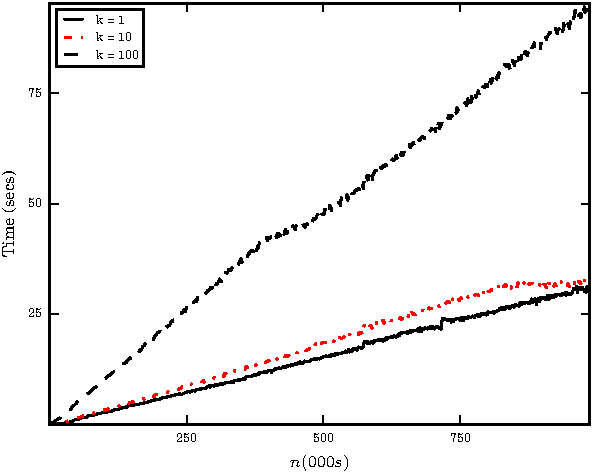
\includegraphics[width=0.65\textwidth]{prox/proxtime-crop.pdf}
\caption{Time taken to compute $\mathbf{prox}^{H}_{g}(x)$ versus $n$, for
  $k=1, 10, 100$; see~\eqref{eq:proxtime}.}
\end{figure}


\subsection{Synthetic least-square problems}

The next set of examples all involve the least-squares objective
\begin{equation}\label{eq:ls-objective}
  f(x) = \tfrac{1}{2}\|Ax-b\|^2_2.
\end{equation}
Two different procedures are used to construct matrices $A$, as
described in the following sections. In all cases, we follow the
testing approach described by \cite{6399612} for constructing a test
problem with a known solution: fix a vector $x^{\star}$ and choose
$b=Ax^{\star}-A^{-T}v$, where $v\in\partial g(x^\star)$. Note that
\[
\partial(f+g)(x^\star)=A^{T}(Ax^\star-[Ax^{\star}-A^{-T}v])+\partial g(x^{\star})=\partial g(x^{\star})-v.
\]
Because $v\in \partial g(x^\star)$, the above implies that
$0\in\partial(f+g)(x^\star)$, and hence $x^\star$ minimizes the
objective $f+g$.  In the next three sections, we apply $\mathtt{QSip}$ in turn
to problems with $g$ equal to the 1-norm, the group LASSO (i.e., sum
of 2-norm functions), and total variation.

\subsubsection{One-norm regularization} \label{sec:1-norm-reg}

In this experiment we choose $g = \|\cdot\|_1$, which gives the 1-norm
regularized least-squares problem, often used in applications of
sparse optimization. Following the details in Example
\ref{L1_Example}, the system $\mathcal{L}(u)$ is a
diagonal-plus-low-rank matrix, which we invert using the SW identity.

The matrix $A$ in~\eqref{eq:ls-objective} is a 2000-by-2000 lower
triangular matrix with all nonzero entries equal to $1$. The bandwidth
$p$ of $A$ is adjustable, and determines its coherence
\[
\mbox{coherence}(A)
=
\max_{i\neq j}\frac{a_i^T a_j}{\|a_i\|\|a_j\|} = \sqrt{\frac{p-1}{p}},
\]
where $a_i$ is the $i$th column. As observed by \cite{6399612}, the
difficulty of 1-norm regularized least-squares problems are strongly
influenced by the coherence. Our experiments use matrices $A$ with
bandwidth $p=500, 1000, 2000$.

Figure~\ref{Exp_L1} shows the results of applying the $\mathtt{QSip}$ solver
with a memories $k=1,10$, labeled ``QSIP mem $= k$''. We also consider
comparisons against two competitive proximal-based methods. The first
is a proximal-gradient algorithm that uses the Barzilai-Borwein
steplength \cite{BarzBorw:1988,wright2009sparse}.  This is our own
implementation of the method, and is labeled ``Barzilai-Borwein'' in
the figures. The second is the proximal quasi-Newton method
implemented by \cite{NIPS2012_4523}, which is based on a
symmetric-rank-1 Hessian approximation; this code is labeled
``PG-SR1''. The $\mathtt{QSip}$ solver with memory of 10 outperforms the other
solvers. The quasi-Newton approximation benefits problems with high
coherence ($p$ large) more than problems with low coherence ($p$
small). In all cases, the experiments reveal that the additional cost
involved in evaluating a proximal operator (via an interior method) is
balanced by the overall cost of the algorithm, both in terms of
iterations (i.e., matrix-vector products with $A$) and time.


\begin{figure}[t]
  \centering
  \begin{tabular}{@{}c@{\ }c@{}}
   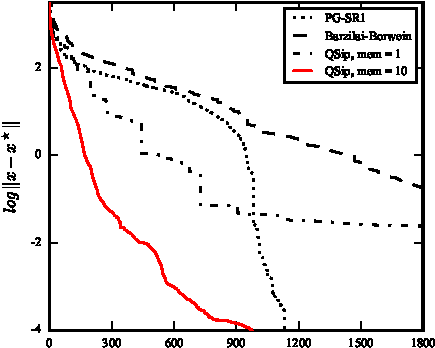
\includegraphics[width=0.44\textwidth]{prox/tang_results_L1-crop}
  &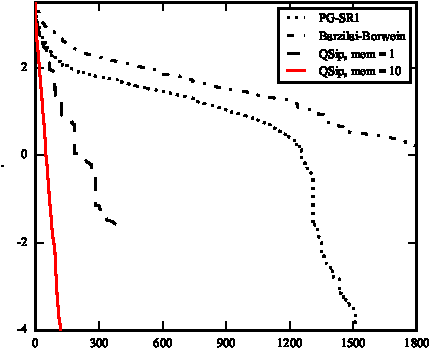
\includegraphics[width=0.44\textwidth]{prox/tang_results_L1_iter-crop}
 \\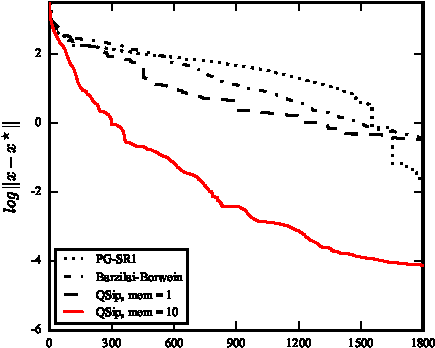
\includegraphics[width=0.44\textwidth]{prox/tang_results_L1_1000-crop}
  &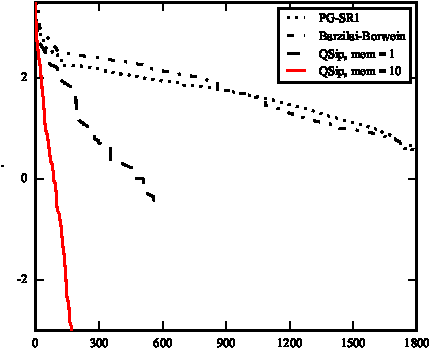
\includegraphics[width=0.44\textwidth]{prox/tang_results_L1_1000_iter-crop}
 \\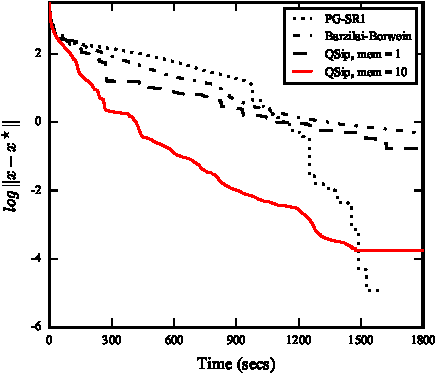
\includegraphics[width=0.44\textwidth]{prox/tang_results_L1_500-crop}
  &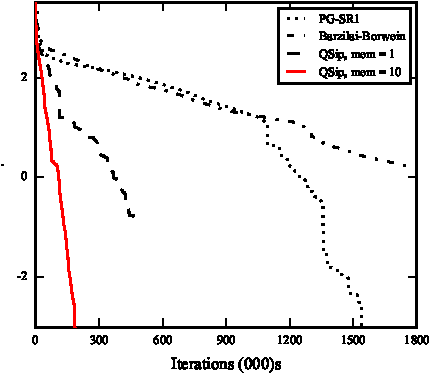
\includegraphics[width=0.44\textwidth]{prox/tang_results_L1_500_iter-crop}
  \end{tabular}
  \caption{Performance of solvers applied to 1-norm regularized
    least-squares problems of increasing difficulty. The left and
    right columns, respectively, track the distance of the current
    solution estimate to the true solution versus time and iteration
    number.  Top row: $p=2000$ (highest coherence); middle row:
    $p=1000$; bottom row: $p=500$ (lowest coherence).   
    \label{Exp_L1}}
\end{figure}

\subsubsection{The effect of conditioning}
\label{sec:conditioning}

It is well known that the proximal-gradient method converges slowly
for ill conditioned problems. The proximal L-BFGS method may help to
improve convergence in such situations. We investigate the observed
convergence rate of the proximal L-BFGS approach on a family of
least-squares problems with 1-norm regularization with varying degrees
of ill conditioning. For these experiments, we take $A$
in~\eqref{eq:ls-objective} as the 2000-by-2000 matrix
\[
A = \alpha_L \begin{pmatrix}
 T & 0\\
0 & 0
\end{pmatrix} + \alpha_\mu I,
\]
where $T$ is a 1000-by-1000 tridiagonal matrix with constant diagonal
entries equal to 2, and constant sub- and super-diagonal entries equal
to ${-}1$. The parameter $\alpha_L/\alpha_\mu$ controls the
conditioning of $A$, and hence the conditioning of the Hessian $A^T A$
of $f$.

We run L-BFGS with 4 different memories (``mem''): $0$ (i.e., proximal
gradient with a Barzilai-Borwein steplength), $1$, $10$, and $100$.
We terminate the algorithm either when the error drops beneath
$10^{-8}$, or the method reaches $10^3$ iterations. Our method of
measuring the {observed convergence} (OC) computes the line of best
fit to the log of optimality versus $k$, which results in the quantity
\[
\mbox{Observed Convergence}
:= \frac{\sum_{k=0}^{N}k\cdot\log \|x_{k}-x_{*}\|}{\sum_{k=0}^{N} \log \|x_{k}-x_{*}\|},
\]
where $N$ is the total number of iterations.

The plot in Figure~\ref{fig:convergence} shows the ratio of the OC for
L-BFGS relative to the observed convergence of proximal gradient
(PG). This quantity can be interpreted the amount of work that a
single quasi-Newton step performs relative to the number of PG
iterations. The plot reveals that the quasi-Newton method is faster at
all condition numbers, but is especially effective for problems with
moderate conditioning. Also, using a higher quasi-Newton memory almost
always lowers the number of iterations. This benefit is most
pronounced when the problem conditioning is poor.

Together with \S\ref{sec:timeprox}, this section gives a broad picture
of the trade-off between the proximal quasi-Newton and proximal
gradient methods. The time required for each proximal gradient
iteration is dominated by the cost of the gradient computation because
the evaluation of the unscaled proximal operator is often trivial. On
the other hand, the proximal quasi-Newton iteration additionally
requires evaluating the scaled proximal operator.  Therefore, the
proximal quasi-Newton method is most appropriate when this cost is
small relative to the gradient evaluation.

\begin{figure}
\centering
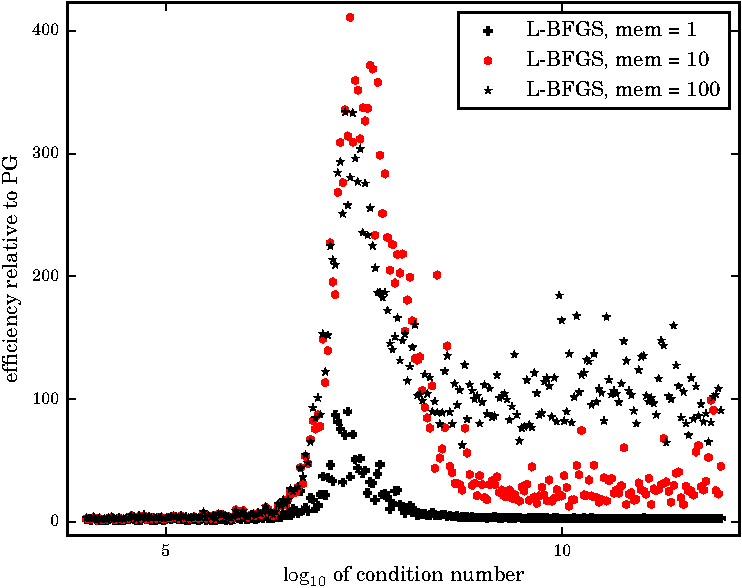
\includegraphics[width=0.65\textwidth]{prox/cond-crop}
\caption{Performance of the proximal quasi-Newton method relative to
  proximal gradient for problems of varying condition number.}
\label{fig:convergence}
\end{figure}
% paragraph paragraph_name (end)


\subsubsection{Group LASSO}

Our second experiment is based on the sum-of-norms regularizer
described in Examples~\ref{ex:sum-of-norms}
and~\ref{ex:group-lasso-cont}. In this experiment, the $n$-vector
(with $n=2000$) is partitioned into $p=5$ disjoint blocks of equal
size. The matrix $A$ is fully lower triangular.

Figure~\ref{Exp_L2} clearly shows that the $\mathtt{QSip}$ solver outperforms
the PG method with the Barzilai-Borwein step size.  Although we
required $\mathtt{QSip}$ to exit with a solution estimate accurate within 6
digits (i.e., $\log\|x-x^*\| \le 10^{-6}$), the interior solver
failed to achieve the requested accuracy because of numerical
instability with the SW formula used for solving the Newton
system. This raises the question of how to use efficient alternatives
to the SW update that are numerically stable and can still leverage
the structure of the problem.
\begin{figure}
  \centering
  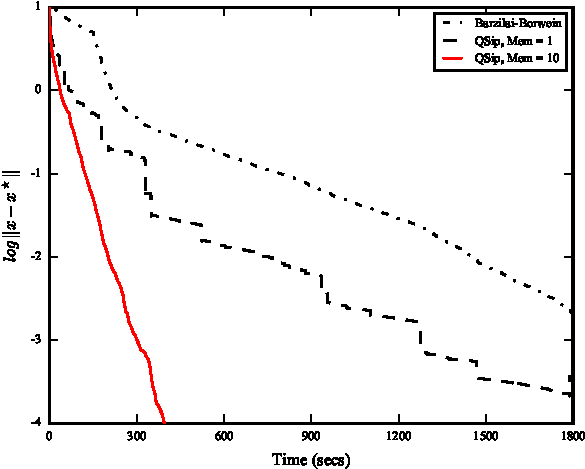
\includegraphics[width=0.65\textwidth]{prox/tang_results_GL-crop}
  \caption{Performance of solvers applied to a group-Lasso problem.
    The horizontal axis measures elapsed time; the vertical axis
    measures distance to the solution.\label{Exp_L2}}
\end{figure}

\subsubsection{1-dimensional total variation} \label{sec:TV} Our third
experiment sets
\[
g(x)=\sum_{i=1}^{n-1}|x_{i+1}-x_{i}|,
\]
which is the anisotropic total-variation regularizer described in
Examples~\ref{ex:graph1-norm-example} and~\ref{ex:graph-1-norm}. The
matrix $A$ is fully lower triangular. Figure~\ref{Exp_TV} compares the
convergence behavior of $\mathtt{QSip}$ with the Barzilai-Borwein proximal
solver. The Python package {\tt
  prox-tv}~\cite{conf/icml/Barbero11,barberoTV14} was used for the
evaluation of the (unscaled) proximal operator, needed by the
Barzilai-Borwein solver. The $\mathtt{QSip}$ solver, with memories of 1 and 10,
outperformed the Barzilai-Borwein solver.
\begin{figure}
  \centering
  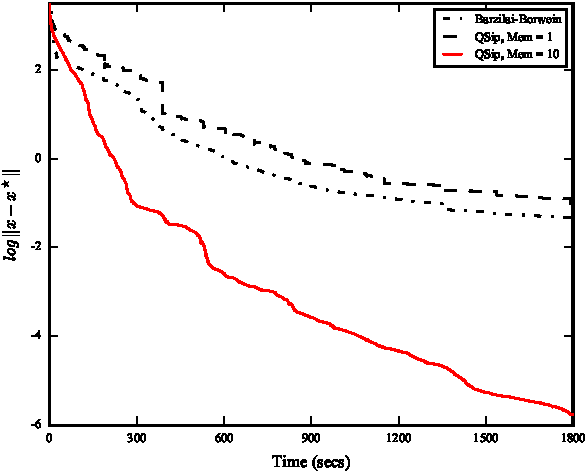
\includegraphics[width=0.65\textwidth]{prox/tang_results_TV-crop}
  \caption{Performance of the $\mathtt{QSip}$ solver applied to a 1-dimensional
    total-variation problem.} \label{Exp_TV}
\end{figure}

\subsection{Sparse logistic regression}

This next experiment tests $\mathtt{QSip}$ on the sparse logistic-regression
problem problem
\[
  \underset{x}{\mbox{minimize}} \quad
  \frac{1}{N}\sum_{i=1}^{N}\log(1+\exp[a_{i}^T x])+\lambda \|x\|_{1},
\]
where $N$ is the number of observations.  The
\textit{Gisette}~\cite{guyon2004result} and
\textit{Epsilon}~\cite{PascalChallenge2016} datasets, standard
benchmarks from the UCI Machine Learning
Repository~\cite{Lichman:2013}, are used for the feature vectors
$a_i$.
% In the Gisette Dataset, Each
% vector $a_i$ represents a handwritten digit (either ``4'' or ``9'') and the
% logistic-regression problem builds a classifier that attempts to distinguish
% between the two digits. 
% The co-variate vectors $a_i$ in this Gisette set are
% dense, and therefore the gradient is costly to compute.
\textit{Gisette} has $5K$ parameters and $13.5K$ observations;
\textit{Epsilon} has $2K$ parameters with $400K$ observations. These
datasets were chosen for their large size and modest number of
parameters. In all of these experiments, $\lambda = 0.01$.

Figure~\ref{fig:l1logreg} compares $\mathtt{QSip}$ to the Barzilai-Borwein
solver, and to newGLMNet \cite{KimKohLustBoydGori:2007}, a
state-of-the-art solver for sparse logistic regression. (Other
possible comparisons include the implementation of
\cite{Scheinberg2016}, which we do not include because of difficulty
compiling that code.) Because we do not know a priori the solution for
this problem, the vertical axis measures the log of the optimality
residual $\|{x_k - \mathbf{prox}_{g}(x_k-\nabla f(x_k))}\|_\infty$ of the
current iterate. (The norm of this residual necessarily vanishes at
the solution.)  On the \textit{Gisette} dataset, Barzilai-Borwein and
newGLMNNet are significantly faster than the proximal quasi-Newton
implementation. On the \emph{Epsilon} dataset, however, the
quasi-Newton is faster at all levels of accuracy.

\begin{figure}
  \centering
  \begin{tabular}{@{}c@{\ }c@{}}
   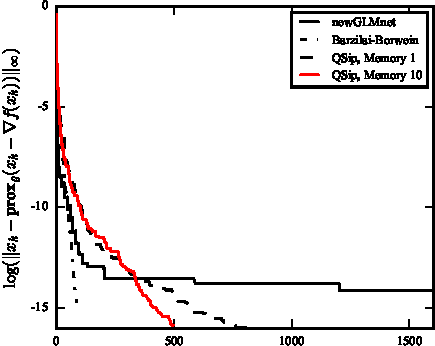
\includegraphics[width=0.485\textwidth]{prox/logistic-crop}
  &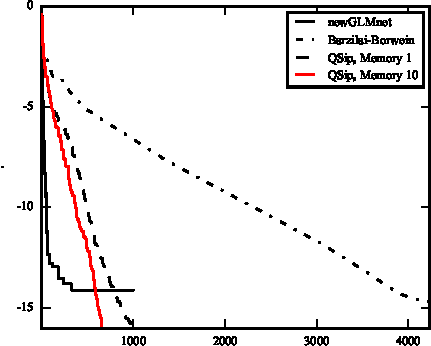
\includegraphics[width=0.485\textwidth]{prox/logistic_iter-crop}
 \\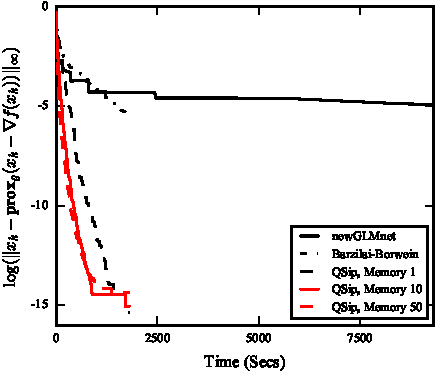
\includegraphics[width=0.485\textwidth]{prox/logistic_eps-crop}
  &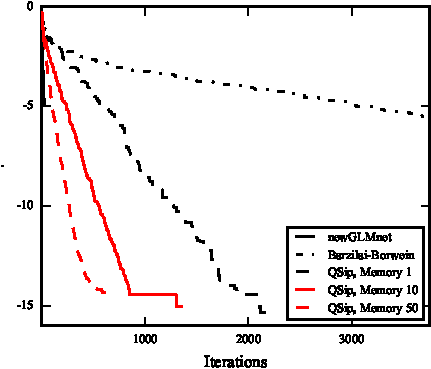
\includegraphics[width=0.485\textwidth]{prox/logistic_eps_iter-crop}
  \end{tabular}
  \caption{Performance of solvers on a sparse logistic-regression
    problem. Top row: \emph{Gisette} dataset; bottom row:
    \emph{Epsilon} dataset. The left and right columns, respectively,
    track the optimality of the current solution estimate versus
    elapsed time and iteration number.}
  \label{fig:l1logreg}
\end{figure}

\section{Conclusion} \label{sec:conclusion}

Much of our discussion revolves around techniques for solving the
Newton systems~\eqref{eq:5} that arise in the implementation of an
interior method for solving QPs. The Sherman-Woodbury formula features
prominently because it is a convenient vehicle for taking advantage of
the structure of the Hessian approximations and the structured
matrices that typically define QS functions. Other alternatives,
however, may be preferable, depending on the application.

For example, we might choose to reduce the 3-by-3 matrix
in~\eqref{eq:5} to an equivalent symmetrized system
\[
 \pmat{-Q & A^T \\ A & D}\pmat{\Delta y\\\Delta s}
   = -\pmat{-{r_d}\\r_p+V^{-1} r_\mu}
\]
with $D:=V^{-1} S$. As described by \cite{benzi2008some}, Krylov-based
method, such as MINRES \cite{PaigSaun:1975}, may be applied to a
preconditioned system, using the preconditioner
\[
  P = \pmat{ -\mathcal{L}(u)  \\ & D },
\]
where $\mathcal{L}(u)$ is defined in~\eqref{eq:mathcalL}. This ``ideal''
preconditioner clusters the spectrum into three distinct values, so
that in exact arithmetic, MINRES would converge in three
iterations. The application of the preconditioner requires solving
systems with $\mathcal{L}$ and $D$, and so all of the techniques discussed
in~\S\ref{sec:eval-prox-oper} apply. One benefit, however, which we have
not explored here, is that the preconditioning approach allows us to
approximate $\mathcal{L}^{-1}(u)$, rather than to compute it exactly, which may
yield computational efficiencies for some problems.
   
   \appendix

   \chapter[A Title of Appendix A]{A Title of Appendix A}
   \label{ch:AppendixALabel}
   %!TEX root = ../Dissertation.tex
\section{Auxiliary results}

\ 
\begin{lem}\label{Terry O} 
  Suppose that
  \begin{align*}
    \phi_{1}(k)&=\mathcal{O}(k^{\mathcal{O}(1)})\exp(-\mathcal{O}(k^{\mathcal{O}(1)})),
  \\\phi_{2}(k)&=\exp(\mathcal{O}(k^{\mathcal{O}(1)}))\exp(-\exp(\mathcal{O}(k^{\mathcal{O}(1)}))),
  \end{align*}
  where $\mathcal{O}(1)$ stands for positive constants. Then for each $A>0$ there exists a positive constant $C_{A}$ such
  that
  \begin{align}
    \phi_{1}(k)&\leq C_{A} k^{-A}, \label{eq:22}
  \\\phi_{2}(k)&\leq C_{A} A^{-k}. \label{eq:24}
  \end{align}
\end{lem}

\begin{proof}
  The statement follows by taking the logarithms on both sides
  of~\eqref{eq:22} and~\eqref{eq:24}.
\end{proof}

\begin{lem} \label{fact:Q-Pochhammer_Lower_Bound}
  For $y\in(0,1)$ and $x\in[0,1]$,
\begin{equation} \label{eq:11}
(1-x)^{1-1/\log y}\leq\prod_{i=0}^{\infty}(1-xy^{i}).
\end{equation}
\end{lem}
\begin{proof}
  To prove the lower bound, we use the following fact:
  \begin{equation*} 
    \ln(1-x)  \geq-\frac{x}{1-x}
    \quad
    \mbox{for all} \quad x\in[0,1).
  \end{equation*}
  Therefore,
\begin{align*}
\prod_{i=1}^{\infty}(1-xy^{i}) & =\exp\left(\sum_{i=1}^{\infty}\log\left(1-xy^{i}\right)\right)\\
 & \geq\exp\left(\sum_{i=1}^{\infty}-\frac{y^{i}}{1/x-y^{i}}\right)\\
 & \geq\exp\left(-\int_{0}^{\infty}\frac{y^{i}}{1/x-y^{i}}di\right)\\
 & =\exp\left(-\frac{\log(1-x)}{\log(y)}\right)
  \geq(1-x)^{-1/\log y}.
\end{align*}
Thus,
\[
\prod_{i=0}^{\infty}(1-xy^{i})  =(1-x)\prod_{i=1}^{\infty}(1-xy^{i})
\ge(1-x)^{1-1/\log y},
\]
as required.
\end{proof}

\begin{lem}
For $y\in(0,1)$ and $x\in[0,1]$,
\[
\exp\left(-\frac{\log(1-x/y)-\log(1-xy^{N+1})}{\log(y)}\right)\leq\prod_{i=0}^{N}(1-xy^{i}).
\]
\end{lem}
\begin{proof}
Similar to the proof of the previous inequality
\begin{align*}
\prod_{i=1}^{N}(1-xy^{i}) & =\exp\left(\sum_{i=1}^{N}\log\left(1-xy^{i}\right)\right)\\
 & \geq\exp\left(\sum_{i=1}^{N}-\frac{xy^{i}}{1-xy^{i}}\right)\\
 & \geq\exp\left(-\int_{0}^{N}\frac{xy^{i}}{1-xy^{i}}di\right)\\
 & \geq\exp\left(-\frac{\log(1-x)-\log\left(1-xy^{N}\right)}{\log(y)}\right).
\end{align*}
Thus,
\begin{align*}
\prod_{i=0}^{N}(1-xy^{i}) & =\prod_{i=1}^{N+1}(1-(x/y)y^{i})\\
 & \geq\exp\left(-\frac{\log(1-x/y)-\log(1-xy^{N+1})}{\log(y)}\right),
\end{align*}
as required.
\end{proof}

\begin{lem} \label{Fact:Tedious_Bound} Let
  $k>0$, $\mu>0$, and $\epsilon>0$. Then for $y\in(0,1)$ and $x\in(0,1]$,
\[
\inf_{\theta>0}\left\{
  \exp(-\theta\epsilon\nu)\prod_{i=0}^{N-1}\left(1-\theta
    xy^{i}\right)^{-k}\right\} \leq
\left(\frac{\exp(1)}{\alpha}\cdot \frac{\epsilon\nu}{x}\right)^{\alpha}\exp\left(-\frac{\epsilon\nu}{x}\right),
\]
where $\alpha=\frac{1}{k}\left(\frac{1}{\log(1/y)}+1\right)$.
\end{lem}
\begin{proof}
  By inverting both sides of~\eqref{eq:11} we obtain the following
  inequality
\begin{equation} \label{eq:Q--LB}
  \prod_{i=0}^{\infty}(1-xy^{i})^{-k}
  \leq
  \exp\left(-\log(1-x)\left[\frac{1}{\log(1/y)}+1\right]\right).
\end{equation}
Therefore, for $\epsilon\geq\alpha x/v$,
\begin{align*}
  &\hspace*{-.5in}\inf_{\theta>0} \left\{
    \exp(-\theta\epsilon\nu)\prod_{i=0}^{N-1}(1-\theta xy^{i})^{-k}
  \right\}
  \\
  &\leq\inf_{\theta>0} \left\{
    \exp(-\theta\epsilon\nu)\prod_{i=0}^{\infty}(1-\theta xy^{i})^{-k}
  \right\}
  \\
  &\overset{(i)}{\leq}\inf_{\theta>0} \left\{ \exp \left( -\frac{1}{k}
      \left[ \frac{1}{\log(1/y)}+1 \right]\log \left( 1-\theta x
      \right) -\theta v\epsilon \right) \right\}
  \\
  &=\inf_{\theta>0} \left\{ \exp \left( -\alpha\log \left( 1-\theta x
      \right) -\theta\epsilon\nu \right) \right\}
  \\
  &\overset{(ii)}{=}\exp \left( -\alpha\log
    \left(1- \left( \frac{1}{x}-\frac{\alpha}{v\epsilon} \right)x
    \right)- \left( \frac{1}{x}-\frac{\alpha}{v\epsilon} \right)
    v\epsilon \right)
  \\
  &= \left(\frac{\exp(1)}{\alpha}\cdot
    \frac{\epsilon\nu}{x}\right)^{\alpha}\exp\left(-\frac{\epsilon\nu}{x}\right),
\end{align*}
where $(i)$ follows from~\eqref{eq:Q--LB}; and $(ii)$ uses the
substitution $\theta=1/x-\alpha/v\epsilon$, which can be shown to be
the optimal choice of $\theta$. Because $\theta>0$, $\epsilon>\alpha
x/v$.
\end{proof}

For the remainder of this section, define the sample average to be
\[
S_{m} := \frac{1}{m}\sum_{i}^{m}X_{i}
\]
for a sequence of random variables $\{X_{1},\ldots,X_{m}\}$.

\section{Sampling Bounds}

\begin{theorem}[{\cite[Theorem~2]{Hoeffding:1963}}]
  \label{thm:Hoeffding Bound} Consider independent random variables
  $\{X_{1},\ldots,X_{m}\}$, $X_{i}:\Omega\rightarrow\Re$. If the
  random variables are bounded, i.e.,
  \[
  d := \sup_{\omega\in\Omega}X_{i}(\omega) - \inf_{\omega\in\Omega}X_{i}(\omega)
  \] is finite, then
  \[
\Pr\left(S_{m}-\mathbf{E}S_{m}\geq\epsilon\right)\leq\exp\big({-2m\epsilon^{2}/d^{2}}\big)
  \]
\end{theorem}


\begin{theorem}[{\cite[Corollary~1.1]{Serfling:1974}}]
  \label{thm:Serfling Bound}
  Let $x_1,\ldots,x_{M}$ be a population, $\{X_{1},\ldots,X_{m}\}$ be
  samples drawn without replacement from the population, and let 
  $$ d
  := \max_i x_{i} - \min_i x_{i}.  
  $$ 
  Then
  \[
  \Pr\left(S_{m}-\mathbf{E} S_{m} \geq\epsilon\right)
  \leq\exp\big({-\epsilon^{2}/\eta_m}\big),
  \quad \text{where} \quad 
  \eta_{m} = \frac{d^{2}}{2m}\left(1 - \frac{m-1}{M} \right).
  \]
\end{theorem}


Because $\eta_m$ is strictly decreasing in $m$, the Serfling bound is
uniformly better than the Hoeffding bound. Note that the Serfling
bound is not tight: in particular, when $M=m$ (i.e., $S_{m} = \mathbf{E} S_{m}$), the
bound is not zero (except for degenerate population).  


   \chapter[A Title of Appendix A]{A Title of Appendix B}
   \label{ch:AppendixBLabel}
   %!TEX root = ../Dissertation.tex

\section{QS Representation for a quadratic} \label{sec:qs-soc}

Here we derive the QS representation of a support function that
includes an explicit quadratic term:
\[
 g(x)=\sup_y\{y^T(B_0x+d_0)-\tfrac{1}{2} y^T Q y \mid A_0y\succeq_{\mathcal{K}_0} b_0\}.
\]
Let $R$ be such that $R^T R = Q$.  We can then write the
quadratic function in the objective as a constraint its epigraph,
i.e.,
\[
  g(x)
  =\sup_{y,\,t}
  \{
    y^T(B_{0}x+d_{0})-\tfrac{1}{2} t \mid
    A_{0}y\succeq_{\mathcal{K}}b_{0},\ \|Ry\|^2 \leq t\}.
\]
Next we write the constraint $\|Ry\|^2 \leq t$ as a second-order cone
constraint:
\begin{align*}
  \|Ry\|^{2}\leq t & \iff\|Ry\|^{2}\leq\frac{(t+1)^{2}-(t-1)^{2}}{4}
\\&\iff
   \|Ry\|^{2}+\left(\frac{t-1}{2}\right)^{2}
    \leq\left(\frac{t+1}{2}\right)^{2}
\\
 &\iff
 \sqrt{\|Ry\|^{2}+\left(\frac{t-1}{2}\right)^{2}}\leq\frac{t+1}{2}\\
 &\iff
 \left\|
   \begin{pmatrix}
     0 & \tfrac{1}{2}\\
     R & 0
   \end{pmatrix}
   \begin{pmatrix}y\\t\end{pmatrix}
  +\begin{pmatrix}-\tfrac{1}{2}\\0\end{pmatrix}
  \right\|\leq\frac{t+1}{2}\\
 &\iff
   \begin{pmatrix}
     0 & \tfrac{1}{2}\\
     0 & \tfrac{1}{2}\\
     R & 0
   \end{pmatrix}
   \begin{pmatrix}y\\t\end{pmatrix}
  \preceq_{Q}
  \begin{pmatrix}
      \phantom-\tfrac{1}{2}
    \\\       -\tfrac{1}{2}
    \\0\end{pmatrix}.
\end{align*}
Concatenating this with the original constraints gives a QS function with
parameters
\begin{equation*}
       A = \pmat{0&\tfrac{1}{2}\\0&\tfrac{1}{2}\\R&0\\A_0&0},
\quad  b = \pmat{{\phantom-\tfrac{1}{2}}\\-\tfrac{1}{2}\\0\\b_0},
\quad  d = \pmat{d_0\\-\tfrac{1}{2}},
\quad  B = \pmat{B_0\\0},
\quad  \mathcal{K} = \mathcal{Q}^{n+2}\times \mathcal{K}_0.
\end{equation*}


   \backmatter

   \bibliographystyle{amsalpha-fi-arxlast}
   \bibliography{master}
   
\end{document}